%!TEX TS-program = xetex
%!TEX encoding = UTF-8 Unicode
\documentclass[11pt,openany]{memoir}

\usepackage{fontspec}
\defaultfontfeatures{Mapping=tex-text}
\setromanfont{Gentium Basic}

\usepackage{geometry}
\geometry{%
    paperwidth=5.25in,
    paperheight=8in,
    top=54pt,
    bottom=68pt,
    inner=54pt,
    outer=45pt,
    footskip=30pt
}

\usepackage[gray]{xcolor}
\definecolor{authorgray}{gray}{0.2}

\makechapterstyle{mainmatter}{%
    \chapterstyle{default}
    \setlength{\beforechapskip}{9pt}
    \setlength{\midchapskip}{0pt}
    \setlength{\afterchapskip}{15pt}
    \renewcommand*{\printchaptername}{}
    \renewcommand*{\printchapternum}{}
    \renewcommand*{\printchaptertitle}[1]{\huge\itshape\centering ##1}
}
\chapterstyle{mainmatter}

\newcommand{\mychapter}[3]{%
\chapter*{#1\\[5pt]{\normalfont\large#2 • #3}}
\addcontentsline{toc}{chapter}{#1\protect\chapternumberline{}}
\addtocontents{toc}{\noindent\hspace{18pt}{\color{authorgray}\itshape\footnotesize #2}\par}
}
\newcommand{\mychaptertoc}[4]{%
\chapter*{#2\\[5pt]{\normalfont\large#3 • #4}}
\addcontentsline{toc}{chapter}{#1\protect\chapternumberline{}}
\addtocontents{toc}{\noindent\hspace{18pt}{\color{authorgray}\itshape\footnotesize #3}\par}
}

%\addtocontents{toc}{\vspace{1em}}

\renewcommand{\cftbeforechapterskip}{.5em}
\renewcommand{\cftchapterfont}{\normalfont}
\renewcommand{\cftchapterformatpnum}[1]{{\normalfont #1}}
\makepagestyle{contents}{}{}{}

\sloppy
\raggedbottom
\pagestyle{plain}
\parindent 18pt

\usepackage[defaultlines=2,all]{nowidow}

\renewcommand{\normalsize}{\fontsize{11pt}{15.0pt}\selectfont}
\renewcommand{\ldots}{\mbox{.\thinspace.\thinspace.}}

\frenchspacing

\usepackage{graphicx}

\hyphenation{Luang Por Pamela Kirby  Matthew Grad Jeff Miller Ila Lewis
Ray Peterson Laurent Palmatier Ruby Grad Shirley Johannesen David
Burrowes Dee Cope Josh Himmelfarb Evan Hirsch Jeanie Daskais John
Nishinaga Wendy Parker Viveka Sumi Shin Jonathan Payne Michael Smith
Khemako Kovilo Pesalo Suhajjo}




\begin{document}

\frontmatter
\addtocontents{toc}{\protect\thispagestyle{plain}}
\pagestyle{empty}

\newcommand{\glosskip}{.6em}
\newcommand\glossentry[2]{\textbf{#1}\hspace{\glosskip}#2\par}
\newcommand\glossentrylang[3]{\textbf{#1} (#2)\hspace{\glosskip}#3\par}

\begin{center}
\vspace*{100pt}
{ \huge Beginning Our Day }

\vspace{20pt}
{ \Large Volume Two}

\vspace{40pt}

{\large
Dhamma Reflections from Abhayagiri Monastery
}

\vfill{}

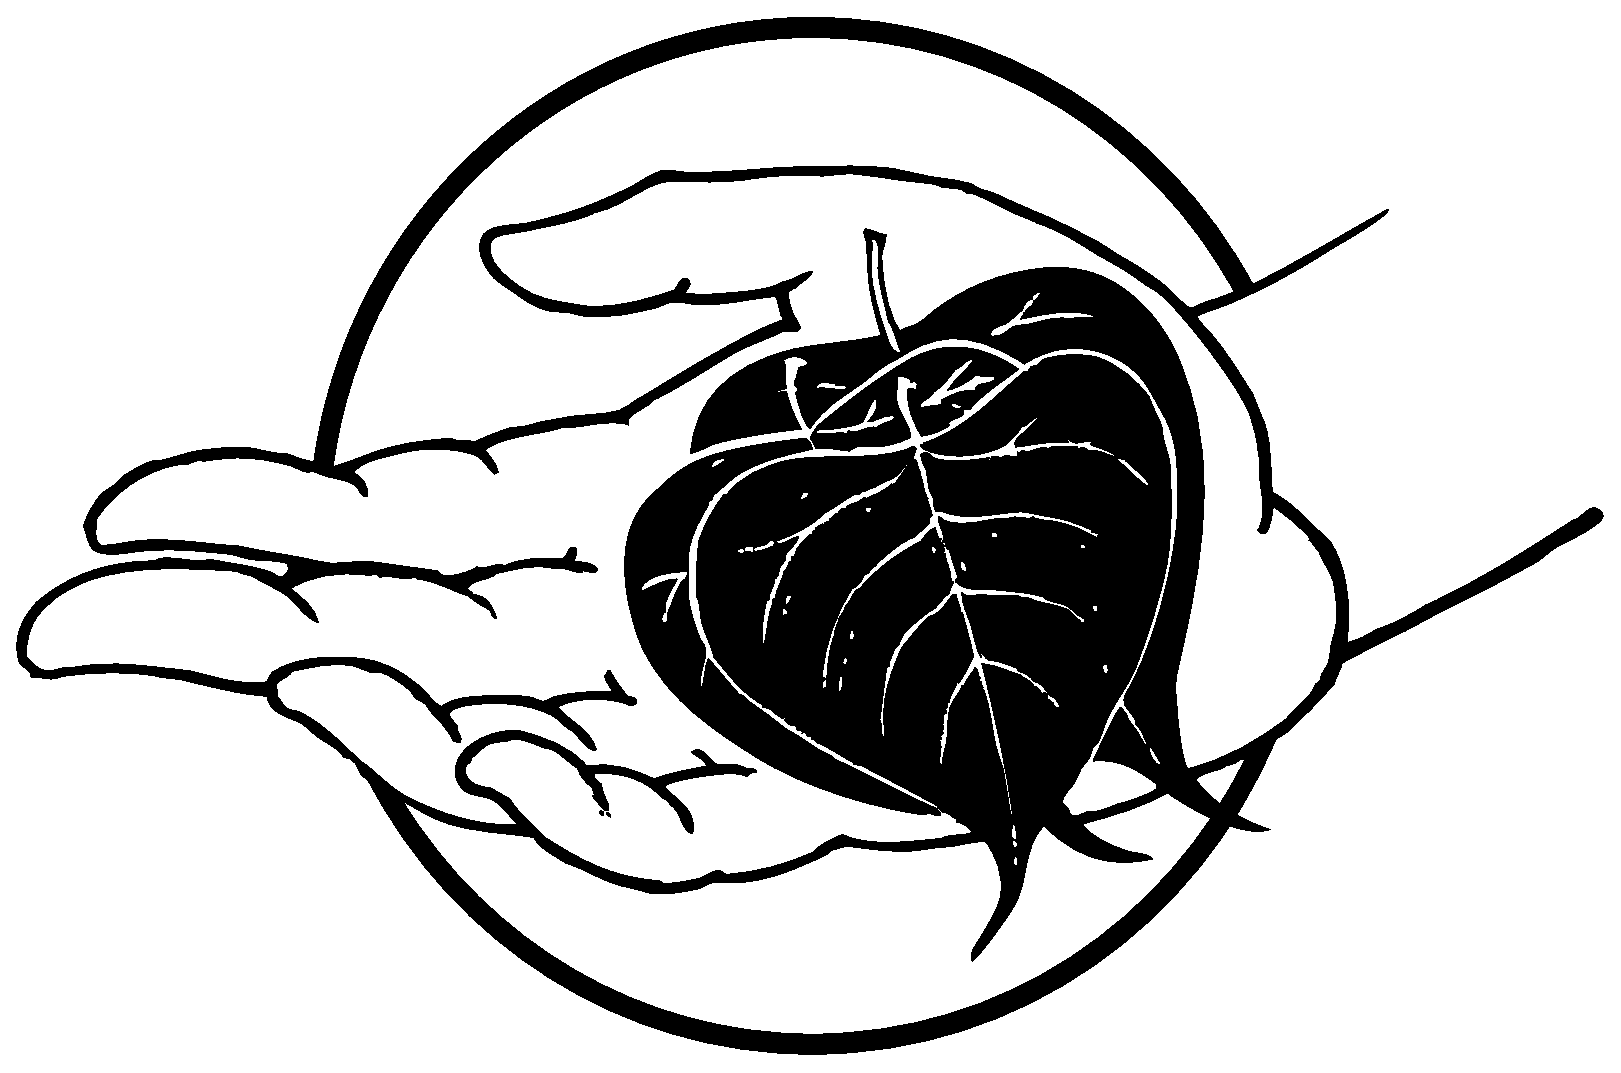
\includegraphics[width=1in]{abm_logo.eps}

\end{center}
\clearpage

\thispagestyle{empty}
{\footnotesize\raggedright
\vspace*{\stretch{1}}

\vspace{1em}
Abhayagiri Buddhist Monastery\\
16201 Tomki Road\\
Redwood Valley, California 95470\\
www.abhayagiri.org\\
707-485-1630

\vspace{1em}
\copyright{} 2014 Abhayagiri Buddhist Monastery

\vspace{1em}
This work is licensed under the Creative Commons
Attribution-NonCommercial-NoDerivatives 4.0 International License.

To view a copy of this license, visit
http://creativecommons.org/licenses/by-nc-nd/4.0/

\vspace{1em}

Interior design by Suhajjo Bhikkhu. Cover design by Sumi Shin.\\
Cover photos by Jonathan Payne. 


\vspace{1em}

We would like to acknowledge the support of the Kataññutā group of
Malaysia, Singapore, and Australia for bringing this book into full
production.

\vspace{1em}

\textit{sabbadānaṃ dhammadānaṃ jināti.}

The gift of Dhamma excels all gifts.
}

\clearpage


\vspace*{\stretch{1}}

This book is dedicated to our teachers and parents.

\vspace*{\stretch{2}}


\clearpage
\mbox{}\clearpage

\pagestyle{plain}
\tableofcontents*


%\thispagestyle{plain}
\clearpage

\thispagestyle{empty}
\mbox{} \clearpage

\chapter{Preface}

``Beginning our day \ldots{}''

These quintessential words are spoken by Luang Por Pasanno before he 
begins each of his morning reflections.

Five days a week, at Abhayagiri's morning meeting, work tasks are 
assigned to the residents and guests living in the monastery. Shortly 
thereafter, one of the senior monks offers a brief Dhamma reflection so 
that the residents and guests have something meaningful to recollect 
throughout their day.

These talks are given spontaneously and often address an event that is 
about to occur, a condition that is already present in the monastery, 
or a general teaching on Dhamma. The most common thread through all the 
reflections is that of practicality: distilling the most important 
teachings of the Buddha into pertinent and applicable practices. Though 
many different teachings are touched upon, the fundamental aim is to 
encourage the abandonment of the unwholesome, the cultivation of the 
wholesome, and the purification of the mind.

While several of these teachings may be read together at one time, 
readers might find it more useful to focus on a single reflection so 
they can easily recollect, contemplate, and make use of it throughout 
their day.

This book was made possible through the contributions of many people. 
Over ten years ago, Pamela Kirby initiated the project when she placed 
a recorder in front of one of the senior monks during a morning 
reflection and proposed that a book be written. Matthew Grad, Jeff 
Miller, Ila Lewis, Ray Peterson, and Laurent Palmatier were the main 
substantive editors of the material, enduring the long and difficult 
process of editing the transcripts into compact and well-written 
teachings. Ruby Grad and Pamela Kirby completed the copy editing. 
Shirley Johannesen compiled the glossary. David Burrowes, Dee Cope, 
Josh Himmelfarb, Evan Hirsch, Jeanie Daskais, Anagārika John 
Nishinaga, and members of the Lotus Volunteer Group: Wendy Parker and 
Viveka all helped with further refining of the text. Sumi Shin designed 
the cover. Jonathan Payne took the cover photos. Michael Smith tumbled 
the stones for the back cover.

For several years, Khemako Bhikkhu recorded the senior monks' 
reflections. Kovilo Bhikkhu and Pesalo Bhikkhu provided corrections on 
an early draft of the book. Suhajjo Bhikkhu generously dedicated a 
significant amount of time on the overall book design and typesetting 
of the text.

The Kataññutā group of Malaysia, Singapore, and Australia generously 
brought this book into full production.

Any errors that remain in these reflections are my own responsibility.

May these teachings bring insight into the nature of Dhamma and provide 
a pathway toward the development of true peace and contentment.

\vspace{1.2em}

\noindent Cunda Bhikkhu\\
Abhayagiri Monastery\\
Redwood Valley, California\\
May 15, 2014



\chapter*{Abbreviations}
\addcontentsline{toc}{chapter}{Abbreviations}

\begin{tabular}{l l}
DN & Dīgha Nikāya\\
MN & Majjhima Nikāya\\
SN & Saṃyutta Nikāya\\
AN & Aṅguttara Nikāya\\
Sn & Sutta Nipāta\\
Cp & Cariyāpiṭaka\\
Jā & Jātaka
\end{tabular}


\mainmatter

\mychapter{Avoiding the Second Arrow}{Luang Por Pasanno}{November 2013}

The obvious thing for me right now is carrying this cold around: a 
thick head and not much energy. It's helpful to reflect on the reality 
of illness or discomfort that is natural and happens all the time. What 
comes to mind is the Buddha's discourse on the two arrows. Being struck 
by one arrow is painful, and being struck by a second one is painful as 
well. In terms of feeling, because each of us has a body, it is quite 
natural that we experience unpleasant sensations. And due to having a 
mind, it is also natural that we are sensitive to the sense contacts we 
experience. These are qualities of the first arrow. Becoming averse, 
worried or anxious about unpleasant feeling---or planning and 
proliferating about how to escape from sense contact---is the second 
arrow.

We can't avoid the first arrow, but we can avoid the second arrow. 
Because we have physical bodies, because we exist, our bodies naturally 
get ill and our minds change. There are always going to be certain 
elements of unpleasant feelings. Even the Buddha himself experienced 
unpleasant feelings and had physical ailments, like a bad back. There 
are places in the suttas where the Buddha turns over his teaching role 
to either Ānanda or Sāriputta because his back is too sore to 
continue sitting and teaching.

We can recognize and be attentive to the first arrow and not turn that 
arrow into something that then creates more complication, difficulty, 
and pain. We can reflect on that as we go about the day, asking 
ourselves, \emph{What are my reactions to unpleasant feelings? What are 
my habits and tendencies?} We can develop mindfulness and discernment 
to receive the first arrow skillfully and not look for ways to be 
struck by the second, third, or fourth arrow.

\mychapter{The Importance of Koṇḍañña's Insight}{Ajahn 
Amaro}{November 2008}

In the Dhammacakkapavatana Sutta, the Discourse on the Turning of the 
Wheel of Dhamma, the Buddha addressed the five \emph{samaṇas}, 
including one named Koṇḍañña, who were his practice companions 
before he became a Buddha. At the end of this talk, the Buddha 
recognized that Koṇḍañña had, with deep insight, understood the 
Dhamma. He said, \emph{``Aññāsi vata bho Koṇḍañño, aññāsi 
vata bho Koṇḍañño ti}---Koṇḍañña understands, 
Koṇḍañña understands.'' Koṇḍañña had awakened to the nature 
of Dhamma: \emph{``Dhammacakkhuṃ udapādi}---the eye of Dhamma 
arose.'' Then the sutta describes exactly what it was that 
Koṇḍañña saw. It wasn't a spectacular vision of the heavens 
opening up, a bewildering light display that he experienced, or streams 
of deities beaming down from the heavens. Rather, his vision of the 
Dhamma was stated simply in the phrase, \emph{``Yaṅkiñci 
samudayadhammaṃ sabbantaṃ nirodhadhamman ti}---whatever is subject 
to arising is subject to ceasing.''

On a worldly level this seems completely unremarkable. That which 
begins, ends. Whatever goes up, must come down. If it's born, it dies. 
\emph{No big deal,} we might think. But it's worth our reflection: This 
seemingly simple insight, which makes all the difference in the life of 
Koṇḍañña, which enables him to awaken to the Dhamma, enter into 
the stream of Dhamma, thus making full enlightenment absolutely certain 
from that point on. Why should that be the most profound insight?

It's helpful to reflect on this and use it as a theme of meditation. 
\emph{Why would it change my life to see that all that is subject to 
arising is subject to ceasing? If that's truly known and understood by 
me, why should that mean that full enlightenment is inevitable, that in 
a certain amount of time it will ripen in my complete and total 
liberation? How can that understanding be so important?} We can 
practice picking up that theme, applying it and seeing it clearly for 
ourselves. It's not simply a collection of words that we hear, \emph{Oh 
yeah, ``All that's subject to arising is subject to ceasing.'' Yeah, I 
know all that.} We can practice exploring it and applying it, moment by 
moment, throughout the day. \emph{Why should that be so liberating? Why 
should that be so significant? Why should that be the change of vision 
that alters my whole way of life, my whole way of seeing who and what I 
am?} This is for all of us to investigate.

When we apply this insight to everything---to what we think, to what we 
feel, to the pleasant experiences, the painful experiences, the 
beautiful, the ugly, the emotionally pleasing, the emotionally 
distressing---it awakens a sense of the nature of experience itself. We 
begin to see that when we aren't judging life in worldly terms---good, 
bad, right, wrong, me, you, beautiful, ugly, in here, out there---then 
we're seeing everything in terms of its nature rather than its content 
or whether we like it or we don't like it, whether we call it in here 
or out there. We awaken to that intuition within us that everything 
internal and external, mental and physical, is part of a natural order. 
It's not self. It's not who or what we are. It's not personal. It's not 
alien. It's just Dhamma. It's nature itself. This understanding 
undercuts the way we see ourselves as, ``Me in here, the world out 
there.'' We no longer believe that those perceptions reflect the way 
things truly are.

This insight seems like nothing, doesn't it? Our ego-centered thinking 
reacts like it's oxygen: \emph{Big deal. There's a lot of oxygen about, 
so what?} But when we are denied oxygen, then it quickly becomes 
apparent how crucial it is. In a similar way, when we apply this 
insight to how we experience our thoughts, feelings, and perceptions, 
then it changes the whole way we hold things. We can notice that change 
within the heart. \emph{Oh right, this is a changing thing. I can call 
it good or bad. I can call it success or failure. But its primary 
quality is that it's changing. It came into being and now it's ending. 
That's the most important thing about it.} We notice that shift in the 
heart, that shift that happens within us when we apply Koṇḍañña's 
insight. It changes everything because we're no longer 
obsessing---fixating on the content of experience. We're becoming aware 
of the process of experience itself.

That's fundamentally what insight, \emph{vipassanā}, is about. 
Vipassanā is insight into the nature of experience itself---that 
moment of clear seeing when there's a direct awareness of how 
experience works, what experience is. And the result of that is 
liberation. At that moment the heart knows, \emph{This is merely a 
pattern of nature, a coming, a going---changing. That's all it is. 
That's all it can be. Nothing to get excited about. Nothing to get 
alarmed about.} Right there is the moment of freedom in seeing clearly 
that the heart is unburdened. There is an unentangled knowing, at least 
to some small degree. That liberating quality is right here, in the 
midst of everyday activity, mundane thoughts, and feelings. Just like 
Koṇḍañña, it is possible for us to access this liberating insight 
right here and right now.

\mychapter{Refocusing on the Defilements}{Ajahn Yatiko}{May 2012}

One of the problems we come across is the tendency to forget the goal 
of our practice and life---in other words, the direction where we 
should be aiming. We need to frequently return to the basic intention 
to be free from the defilements of greed, hatred, and delusion, because 
it's so easy to get caught up in the conditions of daily life, wanting 
the conditions to be a certain way, either liking our present 
conditions or disliking them. People who are active, work a lot, 
coordinate a lot, or do a lot of planning can easily spend the whole 
day manipulating conditions, especially if they are skilled at this.

I once knew a German monk in Thailand who candidly said to me that he 
could look at anything, for instance a water fountain, and tell me five 
things that were wrong with it. He said he could look at anything and 
tell me how to improve it, whether it's in the wrong place, designed 
poorly, or not properly cared for. He said this in a sweet, 
non-boasting way. It's easy for people with that ability to believe 
that they can sort out all the conditions. Sometimes things truly 
aren't working well or people aren't behaving the way they should, and 
in our minds we think we can get it all sorted out. But when we try, it 
doesn't usually work out the way we want. Or if it does, that can be 
even worse, because then we're not likely to have been aware of the 
defilements that came up when we attached to our view about the right 
way of doing things.

It's as if we have a spotlight of awareness focused on external 
conditions, applying strong views and judgments about the way things 
are or should be. This can create a great amount of suffering in some 
cases. Basically, we're looking in the wrong place. We can spend our 
whole lives focusing outward, trying to get things, situations, or 
people to do what we want, forgetting that our awareness and perception 
should be focused inwardly, on ourselves. In our tradition it's been 
said that as monastics 95 percent of our focus should be on our own 
state of mind, our own movements of mind. We focus internally because 
we want to be free from suffering and this is how we accomplish this 
task.

Not long ago we drove up to the Old Gold Mine Hermitage and in the van 
I listened to a classic talk from Ajahn Jayasāro. It's called 
``Recognizing the Upakkilesas.'' In this talk, he analyzes various 
defilements of the mind such as anger, ill will, cruelty, envy, 
belittling, and self-righteousness. As I listened, a mood of irritation 
came up, and I started investigating what this irritation could be and 
how I could describe its nature. To really describe a defilement we 
need to study it. For myself, it's not so helpful to study defilements 
intellectually, as in the Visuddhimagga, where each defilement is 
defined as having specific attributes and proximate causes. Instead, 
the way of study I find most helpful in practice is through direct 
experience. So with irritation, for example, we study what's going on 
right now, once irritation has arisen. We investigate what it's all 
about, what it feels like, and what conditions gave rise to it in this 
specific case. Doing this, we can clearly see that the conditions which 
gave rise to irritation will change, and that irritation will arise 
again in another situation if those same conditions are present.

We can use whatever arises as an object of study. Taking an extreme 
hypothetical situation, let's say an anagārika calls me ``Ajahn 
Fatico,'' and I get upset about this, thinking what he said was 
inappropriate and insulting. Let's say this gives rise to anger, and I 
really want to set him straight. However, in terms of my own practice, 
the fact that he insulted me is not the point at all because even if I 
do set him straight and he apologizes, in the future I may feel hurt or 
angered by a comment somebody else makes---I've done nothing to prevent 
that hurt and anger from arising when the same conditions recur. It's 
an endless cycle for us if we go about things in this way. So we need 
to change our focus from being set on external conditions, such as what 
other people say and do, and instead focus on the way our attachments, 
cravings, and defilements move through experience. We can see that they 
aren't ours---they don't belong to us. We need to recognize and 
appreciate that.

The Pāḷi word \emph{āgantuka} means newcomer or guest. An āgantuka 
monk is a visiting monk who comes from a different tradition, who may 
have different standards of Vinaya, or who does not know the way we do 
things here. In one sutta passage, the Buddha says that the defilements 
are visitors---that the mind is intrinsically pure, and the defilements 
come into the mind as āgantuka (AN 1.49). So the defilements are 
merely visitors, they don't really belong in the mind. We have to see 
how these defilements arise and pass away, how they're not part of us 
and don't define who we are. To see that takes attention, focus, and a 
clear sense of what our priorities are in the practice.

\mychapter{One Breath at a Time}{Luang Por Pasanno}{June 2012}

Distributing the daily work assignments seemed a bit complicated today. 
That's the nature of organizing many people living together. When there 
is one person living in one place, it's fairly simple. With two people 
it's a little harder, and it gets exponentially more complicated as the 
number of people increases.

For this reason, we need to learn the skills of living together, so 
that our own interactions and how we relate to each other don't get 
overly complicated. And in general terms, as practitioners, it is 
essential that we cultivate the quality of simplicity in the ways we 
relate to things. In reality, there is one moment at a time, and we 
take one step at a time when we do things. It's not all that 
complicated.

But the mind tends to leap forward toward proliferation, so we need the 
patience to step back and ask ourselves, \emph{What do I have to deal 
with right now?} Mostly all we have to deal with right now is breathing 
in and breathing out. There's not much to do. If there is a task to be 
done, then we can learn how to apply patience and attention to it. We 
put attention on what we are doing, the way it impacts the people 
around us and the circumstances we are in.

As we do this, we realize that the morning has passed, another day has 
moved on. Very simple. We can recall this quality of simplicity as we 
pay attention to the reactions in the mind, the moods that keep popping 
up, and the proliferations that keep hounding us. We can remember: 
\emph{One breath at a time, one step at a time.} It's all very 
uncomplicated and there's not much to be done.

\mychapter{Brightening the Mind}{Ajahn Karuṇadhammo}{August 2012}

Recent discussions and Dhamma talk reflections have focused on the 
theme of right effort. Many of us can be so caught up in what we think 
of as Dhamma practice or meditation practice that we create a narrow 
focus for ourselves. Several of us here came to Buddhism with a focus 
on the practice of meditation in the context of silent retreat, 
oftentimes with a very specific technique related to quieting the mind. 
Sometimes it's easy to get the idea that Buddhist practice boils down 
to right concentration or a specific meditation method. But the 
Buddha's Eightfold Path is much broader than that. Right effort, one of 
these path factors, is a significant skill to be developed. With right 
effort, we are learning to be sensitive to the effect our minds have on 
what it is we're doing. We are examining and asking ourselves, 
\emph{Are wholesome states increasing or unwholesome states 
decreasing?} That's our benchmark. That's our measure of whatever it is 
we're doing in what we call our Buddhist practice.

For instance, the theme today for Upāsikā Day, ``Brightening the 
Mind,'' focuses on the formal side of meditation, which is often---but 
not explicitly---talked about in terms of contemplation. There are many 
kinds of active reflections the Buddha gave to help prepare, brighten, 
and soften the mind. By building on those qualities we can develop more 
refined states of concentration. So that is our orientation---to learn 
how to develop and prepare the mind, not only with formal meditation 
practice, but also in our daily activities.

The rest of the path is oriented toward the other supports and 
developments of right view and the attitudes and actions that are part 
and parcel of our practice to liberate the mind. We follow this path by 
paying attention to whatever it is we are doing, in the livelihood 
we've chosen and in the activities and various ways we express 
ourselves in body, speech, and mind. We can ask ourselves if what we 
are doing or thinking is leading toward wholesome states of 
mind---toward more peace, contentment, and satisfaction, or toward less 
stress, suffering, clinging, and holding on to unskillful habits of 
responding in the world. We can use that as the benchmark around all of 
our activities, everything we do. This in turn allows us to let go of 
the belief that meditation or practice is something we do only after 
our activities are done, when we get up to our \emph{kuṭis} or find a 
place to sit quietly. We are gaining insight into the perspective that 
it's all practice right here and right now, toward the increasing of 
wholesome mind states and the decreasing of the unwholesome ones.

\mychapter{The Benefits and Drawbacks of Change}{Luang Por 
Pasanno}{October 2012}

There is a feeling of change today since the rain has come. The rain on 
the roof is an unfamiliar sound after months and months of dry summer. 
As I came down this morning for \emph{pūjā}, there was the smell of 
moisture in the air. We can pay attention to that feeling of change.

The mind tends to look at things from a one-sided perspective. We might 
be people who love the warm summer and hate the cold rainy time, or we 
might like the colder wet weather and hate the heat. But nothing is 
ever one-sided like that. Everything has its benefits and drawbacks, 
and the Buddha instructs us to investigate that.

This includes investigating the drawbacks of things we like and are 
excited about. It's starting to get cool, the dust has settled, the 
plants are coming out, and the forest is regenerating---these are the 
benefits of this lovely weather. At the same time, a gutter is leaking 
and dripping down the side of the wall onto the deck and needs to be 
repaired.

There was a group of Pa-Auk Sayadaw's lay disciples who were planning 
on coming up today to have a look at Abhayagiri. They were thinking 
about how to develop their new property for Pa-Auk and were excited to 
see what we've done here. However, we received an email from them this 
morning saying that with the new rain they found leaks in several of 
their buildings and need to fix them right away. So they have to 
postpone their trip for some time.

There are benefits and drawbacks to everything. If we think in terms 
of, \emph{I like this} or \emph{I don't like that,} we end up trapping 
ourselves. By looking at experience from a broader perspective and 
applying Dhamma to it, we can more easily recognize that everything has 
two or more sides and see more clearly how problematic it is to take a 
personal position on what we are experiencing. That way we're not 
investing in the I-me-mine of how we think things should be. Rather, 
we're examining the way things are, reflecting on both the benefits and 
drawbacks of the situation.

\mychapter{Snow on a Forest Trail}{Ajahn Jotipālo}{December 2013}

This morning I was walking through the forest on a path that I've 
walked thousands of times before, and everything looked completely 
different. Two conditions had changed: there was moisture in the air 
and the temperature had dropped below freezing. This completely 
transformed the path. Most of the trees were covered with heavy snow 
and ice. It was quite beautiful.

I was contemplating this in terms of the characteristic of not-self, as 
a reminder of how we can take our thoughts, moods, and opinions and 
believe them to be who and what we are. We may have a thought and then 
some reaction, like anger, but that anger is not who we are---it's 
merely a transient phenomenon, like the snow on the trail. It's merely 
the result of some condition that came into being. Whatever habitual 
reactions we may have, they have been conditioned into us. They're all 
due to past causes. And just like snow will melt given a certain 
temperature, when the conditions change for us, our reactions may 
change as well.

I used to be bothered by a couple of people in the community, the way 
they habitually reacted in certain situations. Then one day it hit me 
that those people were merely reacting exactly as they'd been 
conditioned to react in that particular situation. This has given me a 
lot of space around difficult interactions that occur with other 
people, and I've been able to recondition my own habitual reactions. 
When I experience aversion to somebody, I can think to myself, \emph{If 
they could act differently they would act differently.} Or I might also 
think, \emph{When the conditions change, this may no longer be their 
habitual reaction.} It can be that impersonal.

This is something we all can do. When we encounter a situation with 
that sort of wisdom, we can respond with compassion, equanimity, and 
understanding, and not experience the \emph{dukkha} of aversion. We can 
transform our inner landscape, as with the snow fallen on a forest 
trail.

\mychapter{The Dhamma of the Buddhas Is Everywhere}{Luang Por 
Pasanno}{May 2012}

As we engage in activity, we can ground our awareness in the body and 
use it as a helpful anchor for our practice. We do this by having a 
tactile sense of contact with the ground, contact with physical 
movement, and contact with the material world around us. This brings 
awareness into the body, but it's also important how this awareness is 
held. The Buddha's way of teaching and training is through questioning 
and reflection. We're not trying to apply a catechism of, ``The body is 
like this,'' repeating it over and over again. The awareness is an 
exploration, an investigation. We are asking ourselves, \emph{What is 
the experience I'm having? Does it feel comfortable or not? Does it 
feel wholesome or not? Is this what mindfulness is, or not?} This kind 
of questioning is not an intellectual analysis, rather, we are trying 
to use contact as a mirror for reflecting and seeing more clearly.

We should, of course, reflect on the mind as well. \emph{What's my 
mental state right now? What's the intention? What's the volition 
within the mind? Is this skillful or not skillful? How do I create and 
maintain a quality of skillfulness?} This is the kind of investigation 
we can carry with us throughout the day. Whether we are sitting in the 
Dhamma Hall, back at our \emph{kuṭis}, or doing our chores, 
reflecting in this way internalizes our experience. It gives us an 
anchor for recognizing whether we're on track or not, whether we're 
according with Dhamma or have lost the plot.

We need to develop these essential skills so that they permeate every 
aspect of our practice, no matter where we are or what we are doing. As 
Ajahn Chah and so many other teachers have often said, ``The Dhamma of 
the Buddhas is everywhere. We don't have to go to the Pāḷi Canon to 
find it. We don't have to be sitting in a monastery to find it.'' It's 
the ability we have to recognize and see the truth, to see the way 
things truly are. It's everywhere. We can connect with it, we can 
contact it, and we can experience it.

\mychapter{The Kamma of Listening}{Ajahn Yatiko}{July 2013}

Offering a morning reflection like this is a bit like planting a seed. 
What is said needs to be listened to with attention, care, and an open 
mind. When that happens, the seed has been planted in good soil. If the 
mind is not attentive or mindful, if it's off dreaming or thinking, 
then it gets no benefit from the reflection. But if the mind is 
attentive, focused, and keen to extract value, then even if what is 
said is very mundane or something we have heard a thousand times 
before, the mind can still benefit greatly. If we hear a reflection 
with the right attitude and a desire for what is wholesome, then value 
can be acquired even if we're not aware of it.

One of Ajahn Geoff's books is called \emph{The Karma of Questions}. 
That's a fascinating theme to reflect on: What kind of kamma is 
involved in asking questions? It's not so much in getting an answer, 
but in asking the question that we create our kamma. Similarly, we can 
reflect on the kamma that is generated by listening to Dhamma. What 
does it mean to listen to Dhamma? Why is listening to Dhamma such 
profoundly good kamma? It's helpful to contemplate the value of 
listening to reflections and to appreciate receiving reflections even 
though it may sometimes feel as if we just want to get the experience 
over with as quickly as possible. If we listen attentively to Dhamma, 
we can realize insight right at that moment of listening, but also, 
days or even years later this Dhamma can give rise to wholesome 
thoughts, perceptions, and attitudes, planted like seeds in our minds. 
We never know when our listening to Dhamma---that initial seed---will 
bear fruit, but the quality of our listening will ensure the seed is in 
good soil.

\mychapter{Supporting Defilements or Supporting Dhamma}{Luang Por 
Pasanno}{June 2012}

In yesterday's reading, Ajahn Baen emphasized a question that is quite 
commonly asked in the Forest Tradition. It's a very simple question 
that we should consider and contemplate in our practice: \emph{Am I 
supporting the defilements, or am I supporting the development of 
Dhamma?} That very simple contemplation is critical, because our 
preferences and biases don't tend to lead us to question in that way. 
We tend to have thoughts like, \emph{What do I prefer? What do I want? 
What view do I think is right?} Does that support our defilements of 
greed, hatred and delusion, or does it support Dhamma? That's a 
question we don't often ask ourselves. But we need to bring it up, not 
only when we're watching and investigating the mind during formal 
meditation, but also during our day-to-day activities.

What is Dhamma? It has many facets, but importantly, Dhamma is that 
which is aligned with the path leading to the cessation of suffering. 
That's the whole point of the Buddha's teachings---to give us the tools 
to free ourselves from discontent, dissatisfaction and dissonance. When 
the mind or heart is dissonant, we can see that clearly as we become 
aligned with Dhamma. When the mind and heart are each in tune, we can 
feel that right away, reflecting to ourselves, \emph{This feels 
peaceful. This feels clear. This brings happiness and well-being. This 
is the opposite of following my attachments and desires, which always 
leads to dissatisfaction.}

Again, it's important to frequently ask ourselves, \emph{Is this 
supporting the defilements or is this supporting Dhamma?} We ask this 
about our actions and our speech. We ask, \emph{How am I establishing 
mindfulness and inner cultivation?} This is how we develop the Dhamma 
in our hearts and relinquish the defilements of the mind.

\mychapter{So What Am I, Chopped Liver!?}{Ajahn Amaro}{December 2008}

A theme we explored on the Thanksgiving Retreat was ``complaining and 
blaming.'' I thought it would be a useful theme because our culture 
tends toward complaint. \emph{If I'm suffering, then the way to the end 
of suffering is to complain or blame. I'm suffering, therefore it's 
somebody else's fault. I've been treated unfairly. This isn't right. It 
shouldn't be this way.} This is powerful conditioning in our lives. I 
remember a \emph{New Yorker} cartoon with a student asking a monk, 
``You say life is suffering, but isn't it also complaining?'' It's 
useful to take a period of time to reflect on the unconscious or 
semiconscious way we react to the experience of suffering---to reflect 
on the urge to be critical, to be negative, to complain, or to find 
fault in ourselves or in the things around us. While reflecting like 
that, we can broaden our view by inquiring into the matter. \emph{Why 
do I think I shouldn't have to experience this illness, this pain, this 
weather, this food, this person sitting next to me?}

Then we can broaden our view further by consciously evoking a sense of 
appreciation and gratitude for the gifts and opportunities we have in 
our lives. This is a way to catch the mind's habitual movement toward 
criticism or complaint, its movement toward the classic 
glass-is-half-empty attitude. Evoking gratitude goes directly against 
that complaining, criticizing, blaming mind. But we need to make sure 
that this gratitude isn't based on a ``think-pink'' attitude---trying 
to sugarcoat things and pretend that we're not really feeling critical 
or negative. It doesn't help much to paste an artificial expression of 
gratitude on top of a negative mood or a feeling.

We begin with listening to the critical, blaming, or complaining mind, 
and hearing what that mind is saying. What's it coming up with? Is it 
the feeling of being unfairly treated, slighted, left out, or ignored? 
Can we hear the mind's cry of righteous indignation, \emph{So what am 
I, chopped liver!?} We receptively listen to the affronted, hurt, 
wounded, abandoned, irritated feelings, and hear the mind coming up 
with the reactions and thought processes that follow those feelings. We 
are simply allowing this experience to be known---this narrow, painful, 
reactionary state of complaining or feeling slighted. By bringing 
awareness to that, fully knowing its reactive quality, we can recognize 
and inquire, \emph{This is a really painful state. Why would I choose 
to react like this? Why would I want to carry this around and burden my 
heart with this?} We're not saying to ourselves, \emph{Oh, I'm supposed 
to be grateful now, I should plant some gratitude in here.} Instead we 
are simply seeing the painfulness of our narrow, self-centered 
reactions. Once we see this, then the very acknowledgment of that 
painfulness can enable us to let go and relax. In the broadening of our 
views and attitudes, what arises is gratitude. We are able to 
appreciate the bigger picture, the gifts and the lessons we have 
received, and the potential opportunities we have in the world.

\mychapter{Letting Go and Picking Up}{Ajahn Karuṇadhammo}{June 2013}

Many of the practices we hear and read about in our tradition are 
focused on the process of letting go---how we let go of our habits and 
tendencies, as well as objects of mind. We do this to dwell in and 
experience the pure state of awareness that comes from not grasping or 
holding onto anything. This is the ultimate practice on the path: 
letting go of negative tendencies and at the end of the practice, a 
complete release, a complete letting go of everything, including the 
path that has taken us there.

I think it is also true that a substantial amount of the practice---if 
not all of the practice before completely letting go---also involves 
picking up. We learn this skill by discerning what it is we need to let 
go of and what it is we need to pick up and engage with. All the 
obstructions and hindrances to meditation---negative thoughts, 
reactions out of anger, greed, or confusion---are habits that with 
mindfulness we see arise in our minds and then let go of to the best of 
our abilities.

In the same process so much of the path is involved with skillfully 
picking up different positive qualities---the habits of generosity, 
renunciation, energy, patience, truthfulness, determination, the 
practices of virtue, the sublime states of mind: loving-kindness, 
compassion, sympathetic joy, equanimity---all of these are using an 
object that we are picking up, and at least temporarily, holding onto. 
Our learning consists of understanding which different types of mind 
states we can access, which ones we want to let go of, and which ones 
we want to develop further. Letting go and picking up often go 
hand-in-hand so that as we begin to recognize a difficult mind state, 
such as anger arising, we realize it's something we want to let go of 
while at the same time---even simultaneously---we recognize something 
like patient endurance that needs to be picked up. For example, if a 
difficult situation arises, such as a when a challenging person comes 
into our life, we can let go as we recognize the tendency to react out 
of anger while at the same time, we can pick up, develop, and nurture 
patience, the determination not to react, and kindness for the other 
person and for ourselves.

This morning I noticed one of the people in the meditation hall gently 
removing a spider from the room. How many people in the world will go 
to great pains to take a spider out of a room and set it free? Most of 
the time it's a quick stomping of the foot and that's it. This is 
something to pick up on, this type of sensitivity and caring for even 
the smallest of creatures. We can think of it as picking up a skillful 
mind habit. All of these actions have an impact on the mind and the 
heart. In our daily lives, we can explore what it is that's helpful for 
us to pick up, nurture and engage with, as well as what habits we can 
develop that will support us in our practice.

\mychapter{Enjoying That Enough-ness}{Luang Por Pasanno}{June 2012}

It's beneficial for our practice to pay attention to how we use the 
four requisites---robe cloth, food, shelter, and medicine---and reflect 
on how we rely on people's generosity and kindness when we receive 
these offerings. Inner qualities that arise from reflecting in this way 
are contentment and gratitude, which are said to be a source of the 
highest blessings---\emph{maṅgala}. These blessings are not only 
beneficial for us, but beneficial for others as well. People become 
inspired and confident when they see we are using the requisites in a 
wholesome way.

While reading Paul Breiter's book, \emph{One Monk, Many Masters}, I was 
reminded of Ajahn Chah saying, ``I have never seen any rich people in 
the world. I see a lot of people, a lot of visitors, but I've never 
seen any rich people in the world. All I've seen is people who don't 
have enough.'' That's a powerful reflection for us. No matter what the 
external conditions of abundance are, it doesn't actually mean one is 
rich or wealthy, because true wealth is not measured by the material 
goods one accumulates. The richness of one's life---having true wealth 
within the limits of the human condition---comes from having the 
ability to be happy and peaceful within those conditions.

We are learning to find satisfaction with the qualities of contentment 
and gratitude, rather than constantly seeking something more, something 
different, or something other than what we have. That's the way the 
mind usually works. The untrained mind is constantly seeking something 
else, whether it's in the material realm, in the realm of views and 
opinions or even in the realm of meditative states. It's constantly 
looking for something else, not content with what it has or what it's 
experiencing. The problem with the human condition is this constant 
seeking and, of course, not really finding. So we need to learn how to 
be someone who has enough, and to be someone who enjoys that 
``enough-ness.''

\mychapter{The Mood Is Not Who You Are}{Ajahn Yatiko}{April 2012}

There's always a mood present in our experience. It's amazing to think 
how the presence of a mood so completely shapes and conditions both our 
attitude and the way we see things. It's important to have straight 
vision---some sense of what our life is about, what it's for, and what 
it is we aspire to. This vision or aspiration provides a compass when 
moods arise that tear us apart and sometimes throw us into turmoil, 
irritability, anger, depression, or frustration. Various moods and 
emotions, often conditioned by relatively minor events, can arise and 
push us in a direction that's quite different than the major direction 
of our vision, our life, what we actually trust and what makes sense to 
us.

One of the lay residents here at Abhayagiri once talked about an 
interesting juxtaposition. One day, while feeling irritable, he came 
down from the mountain and went into the kitchen. There was a guest 
there who didn't seem to be pulling his weight, which affected this 
resident's mood. Later on that day, he got word that this guest was 
struggling to digest the news that his brother had been shot and 
killed. Juxtaposing reality and perception---the guest's shock and the 
resident's irritation, for instance---can put things into perspective 
and reveal how petty we can be.

It's human to get irritated when things aren't going as smoothly as 
we'd like or when we're feeling misunderstood. But we need to recognize 
that indulging in such moods puts our present and future well-being at 
risk. We have this life and it's not a game. If we let our moods take 
control and spur us to act on impulse, then we wind up doing things 
that can damage our long-term interests and the well-being of others.

So when these unwelcome moods arise, it's important to do everything we 
can to gain perspective on them and remember that they come and go. We 
shouldn't blindly delight in good moods either. It's okay to enjoy a 
good mood, but if we get lost in it then we'll get lost when a bad mood 
comes around as well. There's no way around that. We can't 
realistically say, \emph{I'll take the good moods and forget the bad 
moods.} We train ourselves in meditation with any mood that comes up. 
We take stock of it and remember that the mood is not who we are, as we 
chant in the Anattalakkhaṇa Sutta. When a mood arises, we do our best 
to recognize its existence and then investigate how it may be pushing 
us to act in ways that aren't helpful to our welfare, or the welfare of 
others.

\mychapter{Putting the Four Noble Truths Into Action}{Luang Por 
Pasanno}{April 2013}

As we bring the practice into our daily lives, it's immensely 
beneficial to use the Four Noble Truths when viewing experience---in 
our formal meditation, interactions with others, and engagements with 
various duties. This is not something to save for later---after 
studying the suttas, developing all the \emph{jhānas} and formless 
absorptions, all the psychic powers, we finally contemplate the Noble 
Truths and become enlightened---it's not like that. The Four Noble 
Truths are to be put into practice right now.

To do this, we need to establish a habit of reflecting and 
investigating in a particular way. First, by examining phenomena 
carefully---the quality of experience, and the results that come from 
interacting with experience in the usual way---we find there's always 
some kind of \emph{dukkha}, some kind of suffering, stress or 
discontent. Then we reflect on that, investigating its cause and how to 
bring about its cessation. When applying these steps, we're not viewing 
the world through the lens of self, of me and my problems, me and my 
accomplishments, me and my preferences, me and my views and opinions. 
We're looking instead from the perspective of dukkha, its cause, its 
cessation and the path leading to its cessation. When we view 
experience like that, life becomes very simple and straightforward.

So we lift up that perspective in the mind and practice with it. We're 
not waiting patiently for some intuitive insight to arise 
spontaneously. We need to deliberately train the mind by frequently 
redirecting our attention and reflecting on experience in that way.

The Buddha gives us the practice method of using the Four Noble Truths 
as a lens to depersonalize experience. And when we use the right 
method, he says beneficial results are bound to follow. If we use the 
wrong method, however, our efforts will be futile. To illustrate these 
points, the Buddha offers some humorous similes. For example, he says 
that when we're wrongly seeking the fruits of practice, we're like a 
man seeking milk: knowing that milk comes from cows, he approaches a 
nursing cow, twists her horn, and then wonders why he doesn't get any 
milk. The reason, of course, is that he's using the wrong method. But 
if he were to use the right method by pulling on the cow's udder, then 
the milk would surely flow. In the same way, even if we understand the 
Four Noble Truths in principle, nothing significant will result if we 
keep those teachings in our heads as mere abstractions. That would be 
using the wrong method, because the most essential bit is missing: 
bringing the Noble Truths into our practice. On the other hand, when we 
do put them into practice and apply them skillfully---that is, when we 
use the right method---then we are bound to realize beneficial results.

Paying attention to the method and its application, putting it into 
practice, bringing the Four Noble Truths into our experience, 
reflecting and applying these truths. This is how we can reap the 
fruits of practice.

\mychapter{Doing What's Difficult to Do}{Ajahn Ñāṇiko}{July 2012}

Living in a monastery can be very difficult---eating one meal a day, 
keeping precepts, trying to live and work together as a harmonious 
community. But as Master Hua said, if we want to practice Dhamma, we 
have to do what's difficult, what others would not choose to do. Even 
though most people wouldn't choose to live in this way, there's an 
enormous benefit to what we're doing here. Living in community, we 
learn how to hold things lightly and take responsibility for what's 
happening in our minds.

During the work period, it's easy for one little event to trigger 
anger, irritation, or some sort of desire. If this happens when we're 
interacting with someone, the mind convinces us that it's the other 
person's fault, as if these defilements came from that other person. So 
it's good to remember that irritation, anger, and desires come from 
within our own minds. They arise there and then seek external objects 
to latch on to. That's why sometimes, no matter how easygoing we may 
be, when we come in contact with some little thing we can become 
irritated---the conditions for that irritation were already there. And 
when we get stuck in irritation or anger with another community member, 
we can forget that it's \emph{dukkha}. We're suffering and the other 
person is suffering too. Sometimes we can get angry at someone else 
because they're angry. This is ridiculous, but it's the way it works. 
The Buddha said, ``If you don't react with anger to an angry person, 
then you win a battle hard to win.'' When interacting with others, we 
may need to swallow our pride from time to time, as difficult as that 
may be.

I remember during my third \emph{vassa} in Thailand, I was doing 
walking meditation every day for several hours after the meal. There 
was a lot of doubt coming up. I was literally driving myself to tears 
with constant doubts in the mind. There I was on the walking meditation 
path, no one else is around, and I'm mired in suffering because of this 
unstoppable mental proliferation. That's how it is sometimes. But these 
experiences are good to have---by going through them, we become 
stronger. Even so, it's difficult to do.

Master Hua said that we're aiming to develop a ``long-enduring 
mind''---a mind that can sustain itself through the months and years 
without sinking far down, becoming dark, falling out of the robes, or 
not wanting to be in a monastery anymore. To develop this long-enduring 
mind, we need to come back to peace, to the skillful actions that help 
sustain us, and to the factors of letting go. We need to come back 
again and again, moment by moment. It may be difficult to do, but the 
reward is true freedom.

\mychapter{Responding to Wholesome Crowds}{Luang Por Pasanno}{April 
2013}

We are preparing for the annual \emph{kaṭhina} ceremony today and 
visitors have already started arriving. In terms of our practice, 
everything that happens on occasions like this is merely sights, 
sounds, smells, tastes, touch, and mental objects. We tend to make a 
problem out of sense contact, but it's just that much, nothing more. 
Objectively speaking, what's taking place here? The day begins, there 
is a wave of people and activity that comes in---it arises. The day 
ends, the wave of people and activity goes out---it passes away. It's 
another arising and ceasing---an opportunity to pay attention to the 
way that things come and go.

Of course, there's more to deal with and manage today, because the 
number of visitors will be high. That's the reality of what's 
happening. But we don't need to get excited about it, create a story 
around it, worry about it, or try to get away from it. Rather, we can 
ask ourselves, \emph{How am I holding all of this?} Are we able to 
return to mindfulness, over and over again? Do we have the ability to 
sustain a sense of clarity, discernment, kindness, and well-being? We 
can choose to let go of excitement, confusion, irritation, and 
aversion. Reactions like those are extra and completely unnecessary.

As a monastic community, we're solely dependent on the generosity of 
the lay community, and this is a time when that generosity is being 
vividly displayed. What can we offer as a gesture of appreciation for 
this generosity that gives us the ability to live our lives? It isn't 
through our getting swept up in excitement. It isn't through our 
shrinking away because of irritation. It's through our ability to hold 
a steadiness and clarity in our minds. Our ability to be clear and 
steady has a lot more value than the short-term satisfaction of 
allowing our minds to get swept up in our reactions. This ability is 
the basis for our practice, but also serves as a model for others. And 
that's what the world needs. It's a wonderful gift when people come to 
the monastery and see a model of wisdom operating in a group of people.

There are people coming---that's not an illusion. So help each other, 
pay attention to the situation and look after what needs to be done. Be 
ready to respond with kindness and attentiveness to the people who 
arrive. Express your heartfelt appreciation. These people are here to 
offer support for the monastery. That kind of generosity is something 
to delight in with a sense of gratitude.

\mychapter{Being Willing to Make Mistakes}{Ajahn Karuṇadhammo}{May 
2013}

How much are we willing to learn from our mistakes? This is a crucial 
aspect of the training---the willingness to recognize when we've missed 
the mark, being open to making mistakes. It's not always easy to 
practice in this way. I think many of us here come with conditioning 
around how important it is to be right all the time. We can grow up 
with a sense of shame---\emph{Unless I'm doing everything perfectly all 
the time, then something is wrong with me.} As far as I can tell, there 
are only a few lucky people who learned while growing up that it's just 
fine to make mistakes. In the community here, there are many of us who 
are strong-willed in certain ways. We have plenty of leaders here and 
sometimes it can be difficult for us to break that classic paradigm, 
\emph{The way I think we should do it is the right way.}

How we begin to unravel this paradigm is by learning it's okay not to 
be right all the time, and to use honest self-appraisal to look at 
ourselves. This allows us to say \emph{Okay, perhaps since everybody 
else is doing it a different way, I need to consider that, or a number 
of people are indicating to me that I may have missed the mark---maybe 
I should think carefully about what happened.} This is a sign of 
internal strength. I also believe highly realized people tend to take 
this approach as well. Those who have penetrated the perception of 
not-self can see there is no ``me'' or ``myself'' that needs defending. 
They know it's not a problem if they're not always right.

This comes down to a matter of skill. Either it's a skill we've 
learned, or one we haven't, or perhaps we've partially taken it 
on---but it's nothing personal. As Luang Por Pasanno was saying, even 
the Buddha after his enlightenment was constantly readjusting. 
Sometimes he'd set down rules, only to realize later they needed to be 
changed. In those cases he would call the monks together, explain the 
need to alter a rule, and adjust it accordingly. Right after his 
enlightenment, the Buddha was inclined not to teach. As the story goes, 
the Brahmā God Sahampati realized this was the Buddha's inclination, 
came down from the brahmā realm, appeared before the Buddha and said, 
``Please reconsider this. There are those who can learn!'' The Buddha 
thought, \emph{Maybe there is a possibility of teaching others how to 
realize what I have realized.} So even at that point he readjusted, and 
he certainly didn't take it personally.

This is a good reflection to bring to mind. Essentially, it's a 
reminder to be honest with ourselves---whether it's relating to 
community life, the monastic discipline, the training, the views and 
opinions about how things should be done, or one's personal meditation 
practice---we can strive for a more open and balanced point of view. We 
do this by honestly looking at our internal experiences, allowing 
ourselves to be present with our fears of being wrong, and saying to 
ourselves, \emph{Okay, I need to make a change; I need to adjust.} And 
then simply let it go and make the adjustment. Once that's done and the 
change has been made, we can move on and not worry about it so much.

\mychapter{A Foundation of Love and Acceptance}{Ajahn Yatiko}{August 
2013}

In this community at Abhayagiri, we need to take care of each other. If 
we don't have a foundation of love and care for each other, then the 
foundation of our lives is on very shaky ground.

I have a tremendous amount of respect and affection for each person 
here, no matter what their personality traits may be. It is important, 
I believe, that we give each other the space needed to be who we are. 
We conform externally; we have these robes, shave our heads, and look 
similar. Yet we are all completely different individuals, remarkably 
so. We need to allow everybody to be who and what they are---to be 
themselves. We mustn't start from a position of being unable to accept 
something or someone. The starting point in practice is being able to 
accept other people and to accept ourselves.

With that as a foundation, we then work with the defilements. It is not 
as if we work with the defilements as a condition for accepting 
ourselves---\emph{Once my defilements are under control, then I'll 
accept myself.} No. We start with acceptance, and from there we can 
work with whatever difficulties arise. Likewise, there's no need to 
expect other people to live up to our standards of monastery etiquette, 
harmony, or even our standards for being happy. It is okay to have a 
miserable day, to be gloomy for quite awhile. We are what we are, and 
we can accept each other whether we are happy, sad, anxious, excited, 
or afraid. That is a very good starting position on which we can build 
our practice.

\mychapter{Comfortable in Any Circumstance}{Luang Por Pasanno}{July 
2013}

It looks like it's going to be hot again today. Most of us are 
uncomfortable when it's hot like this. So what we need to do, as Dhamma 
practitioners, is learn how to adapt. We learn to dwell with 
mindfulness and equanimity whether things are to our liking or not. The 
tendency is to wait for conditions we like and when they arise, only 
then do we say to ourselves, \emph{Okay, now I can practice.} It's an 
attitude that can easily become habitual. But being tied to the human 
condition as we are, it's rare for things to be just right. So what we 
need to do is develop a willingness to work with conditions as they 
are. If it's really hot, then we adjust our pace accordingly, perhaps 
we slow down what we're doing. We may say to ourselves, \emph{Really, 
truly, I can't practice now. I have to wait for this to be over and 
then I can practice.} That's a common response, but we shouldn't waste 
our time with it.

Often we deal with imperfect conditions by getting in touch with our 
``inner complainer'' that's whining away, going on and on about how 
miserable we feel. Instead of mindlessly doing that, we can use 
challenging circumstances as a means of investigating the habit of 
complaining. We do this by watching the mind trying to convince itself 
that physical discomfort automatically means we have to experience 
mental discomfort. When the mind is adopting that sort of 
misunderstanding and complaining about the circumstances, we observe 
how this simply perpetuates suffering. It's not that we're trying to 
sugar coat the tendency to complain by saying to ourselves, \emph{Oh, 
isn't this wonderful? I just love it when it's 108 degrees outside.} 
Instead we're facing reality and being honest with ourselves. At the 
same time, we understand that simply because circumstances are less 
than ideal, they do not also have to be a source of complication or 
oppression.

The point is to distinguish between the direct, physical experience and 
the layers of mental complication we add to that experience. When we do 
that, it gives us an inner refuge, allowing us to be comfortable in any 
circumstance. That's one of the magical things about Dhamma practice. 
We can be at ease and clear in any circumstance if we're willing to 
direct our attention in a skillful way.

\mychapter{The Role of Observance Days}{Ajahn Amaro}{August 2008}

The purpose of our weekly Observance Day is to put our usual daily 
tasks down and focus on the precepts and the formal spiritual qualities 
of our life. It's a day of recollecting and observing, of remembering 
the Dhamma and our original motivation for being here at the monastery. 
It's a time to remember the possibility we have as human beings to let 
go of all confusion, delusion, aversion, greed, and self-centeredness. 
It's a time for renewing our motivation and to begin again fresh.

As monastics, we shave our heads, taking the hair back to the root, 
back to the source, to begin again. There's that quality of tidying 
up---cleaning the shrine room, cleaning the kitchen, squaring things 
away, renewing our precepts. On a practical and symbolic level we're 
keeping the monastery tidy and looking after the things that have been 
offered for our use. On the internal level, we're remembering our 
priorities and helping to clarify the central principles of our lives.

The activities of the Observance Day---taking the precepts, shaving the 
head, having the all-night vigil, and putting aside the work 
routine---are all geared toward reinforcing the reason we're here at 
the monastery. We're not here to construct \emph{kuṭis}, post 
pictures on the website, cook meals, or any of the 10,000 tasks that 
occupy our attention. The whole point of this place existing, this 
gathering of human beings on this particular patch of hillside, is to 
realize the Dhamma---to let go of greed, hatred, and delusion. That's 
the reason we're here. Our preparations for the Observance Day and the 
day itself are all meant to help us to remember, \emph{Oh, right, 
that's what it's all for, of course. Why was I forgetting that?} That's 
the purpose of all the construction projects and committees. That's why 
we take care of these duties and keep the place clean and tidy. That's 
what it's for---the realization of Dhamma.

\mychapter{Blown Into Cosmic Dust}{Luang Por Pasanno}{April 2013}

The Buddha encouraged us to contemplate aging, sickness, and death 
every single day. It's essential that we make an effort do that, 
because the mind's nature is to forget about these contemplations. It 
inclines away from them and instead, inclines toward thoughts of 
eternal youth and health. For the most part, death doesn't exist for 
us. So we have to make it conscious in our practice by realizing the 
limitations of the human condition on the physical level. We're bound 
to this body that's constantly aging. Even when we're young, it's still 
aging. The reason a baby gets born in the world is because it's too old 
to stay in the womb. That aging process continues on after birth.

This is a supportive reflection for us---it's not intended to make us 
miserable or depressed. It's intended to bring up wholesome mental 
states to counteract the mind's tendency toward \emph{pamāda}---being 
careless and not very circumspect regarding the truths of our 
existence. These three recollections help establish a sense of 
heedfulness and spiritual urgency. We have this opportunity to hear the 
Dhamma, to study the Dhamma, to practice the Dhamma, to live a life in 
accord with the Dhamma. Reflecting on that makes us grateful for this 
opportunity to practice and that's vital, because it's easy to let the 
opportunity slip by.

We recollect the nature of the human body---that our lives are subject 
to aging, sickness, and death. For all of our seeming solidity, we're 
left to nature when we die---our bodies dissipate and disappear. The 
Buddha taught the charnel ground contemplations, which encourage us to 
examine the body's process of dissolution after death. It changes 
shape, bloats, disintegrates, and dries out until just the sinews and 
bones are left. The bones are then scattered until there's little 
remaining but a small pile of gray dust. Then a wind comes along and 
blows it here and there until there is nothing left. For all of our 
obsessions about ourselves---our worries, fears and anxieties around 
health and physical well-being, and all the uncertainties in our 
lives---it is absolutely certain that, on a physical level, we're all 
going to be blown into cosmic dust.

Now when we contemplate that fact, it's not to be picked up in a 
nihilistic way, but rather with the sense of urgency that's needed to 
establish the heart within skillful spiritual qualities---the sense of 
urgency we need to keep attending to our actions of body, speech and 
mind, so that they're conducive to clarity, wisdom, and wholesome 
states of mind.

Everyday we recite the Five Subjects for Frequent Recollection. When 
reciting the fifth, we recollect: ``I'm the owner of my kamma, heir to 
my kamma, born of my kamma, related to my kamma, abide supported by my 
kamma. Whatever kamma I shall do, for good or for ill, of that I will 
be the heir.'' These recollections help us establish our kamma---our 
actions of body, speech and mind---in what is wholesome, skillful and 
beneficial, in what bears fruit in terms of peace and clarity, 
happiness and well-being. So it behooves us to take responsibility for 
these contemplations, to reflect upon them and develop them in our 
practice.

\mychapter{When Generosity Motivates Our Practice}{Ajahn Yatiko}{April 
2013}

This morning in meditation I was reflecting on the various offerings 
that have been made to me in my life. It's a really wonderful exercise 
to do from time to time. This sitting cloth was made by Ajahn 
Ñāṇiko. I'm wearing clothes that Dennis gave me. David's mother, 
Ayya Santussika, gave the monastery this vibrating alarm clock. Ajahn 
Jotipālo made this wooden holder for the bell. Ajahn Saññamo gave me 
the socks I'm wearing, which were given to him by Tan Khemako, who 
received them from a layperson. The flowers on the shrine came from our 
friend Apple.

As monastics, it's nice that for almost any material item around us we 
can name the specific person or group of people who offered it. By 
doing this we realize that absolutely everything we have is a gift from 
faithful and generous people. As alms mendicants, we rely on the 
faithful generosity of the laity to provide us with food as well as 
other material supports---robe cloth, shelter, and medicine. Our 
survival is sustained through the gifts of others. When we reflect on 
this, quite naturally the result is a sense of gratitude and 
appreciation.

At the same time, such generosity and support can cause us to ask, 
\emph{Why am I allowing myself to receive all this goodness and 
kindness?} The reason is that having faith in the Buddha's teachings, 
we became intent upon being free from greed, hatred, and delusion, and 
so we came here to devote ourselves to the Buddha's path, which takes a 
great deal of commitment and effort. This is why we receive so much 
goodness from others, which in turn inspires us to practice well.

However, this dynamic can create a problem. Many of us come from a 
strongly guilt-driven culture, and we can say things to ourselves like, 
\emph{Everyone is supporting me, so I should practice hard, I should do 
sitting meditation and walking meditation. I should learn the suttas.} 
For us, the word \emph{should} can mean that if we don't do it, we're 
really bad monks. That's the completely wrong approach. Instead, we can 
reflect that \emph{Since everything is given to me, even this body 
doesn't belong to me. It belongs to the faithful---it's merely loaned 
to me by them.} With that in mind, there's still the sense that we 
``\emph{should}'' practice, but it comes from a completely different 
``\emph{should}.'' It's more like a voluntary ``\emph{should}.'' It 
comes from a wholesome desire to practice because we know that it's 
worthwhile, a decent thing to do. We come to realize, \emph{It's for my 
own benefit, and it's for other people's benefit.}

As we walk on the meditation path, we can contemplate the difference 
between these two kinds of ``shoulds.'' There's a significant 
difference between the ``\emph{should}'' of guilt and the 
``\emph{should}'' of the natural and wonderful activity we're 
interested in doing. We can reflect on the blessings of our lives, the 
things that have come to us, and realize what a wonderful opportunity 
we have to practice and cultivate the path of the Buddha.

\mychapter{Applying a Wholesome Attitude}{Luang Por Pasanno}{May 2012}

Yesterday Ajahn Saññamo gave us a reading about sweeping leaves---how 
sweeping can be an integral part of our practice. His reading came from 
a book detailing the practices at Ajahn Baen's monastery. It is a big 
monastery with large open areas so every day, everybody goes out to 
sweep. In his monastery, sweeping is part of the practice and training. 
That's the way it should be for us as well---and not only with 
sweeping. All the various chores, duties, and responsibilities we have 
are part of the training. They're not simply things to fill the time, 
or excuses to take a break from practice to get something ``practical'' 
done. Rather, they allow us to examine the attitudes we bring to the 
activities we perform and to evaluate the way we spend our time.

How \emph{do} we spend our time? Do we spend it thinking about 
ourselves, and resenting anything that impinges on our preferences, 
views, and opinions of how we imagine things should be? Or do we spend 
our time engaged in what we do with generosity and kindness, with a 
sense of relinquishment? Do we put energy and effort into our chores 
and duties, or do we try to slide by, thinking to ourselves, \emph{If 
people see me moving around the place, maybe they won't notice that I'm 
not really getting much done.} These are some of the attitudes we might 
bring to our practice. It's helpful to skillfully engage with these 
attitudes, because they can give rise to unwelcome, problematic moods. 
Once a mood like that does arise---if we're engaged with what's going 
on---we can respond with an energetic attitude, asking ourselves, 
\emph{How can I shift this mood in a positive way?}

There's a story Ajahn Sumedho tells about sweeping during his early 
days at Wat Pah Pong. It is a standard practice in forest monasteries 
to sweep the grounds, and Wat Pah Pong is no different. The day before 
each Wan Phra, the bell would ring to indicate that it was time for 
sweeping, and all the monks were supposed to go out and sweep the 
large, dusty central areas of the monastery. Ajahn Sumedho relates how 
he didn't like going out into the heat and the dust, nor did he like 
the activity of group sweeping, so he'd usually wait to join the group 
until he was about the last person to come out. Because he took so long 
to join the group, he'd often get the last broom, which was usually 
some scruffy old thing, made of a few little twigs that didn't really 
do much. Ajahn Sumedho said he would go along and scratch a bit at the 
ground, stand, wait, internally grumbling and complaining, saying to 
himself, \emph{This is really stupid. I don't like this. Why do we have 
to do this?} His mind would go on and on. Of course, Ajahn Chah noticed 
what was happening, and one day during the sweeping period he walked 
past Ajahn Sumedho and said, ``Wat Pah Pong---is it suffering?'' Ajahn 
Sumedho reflected on this, \emph{Wat Pah Pong---is it suffering? No, of 
course not! Wat Pah Pong isn't suffering! It's me! It's not Wat Pah 
Pong. I like Wat Pah Pong. I'm the one making suffering out of this. 
It's me.} That was a powerful and significant insight for him---to see 
that the external situation is one thing, and whether or not he adds 
suffering to it is another. After that, Ajahn Sumedho put more energy 
and enthusiasm into the sweeping. By doing so and reflecting, he 
decreased the suffering for himself and turned sweeping into an 
enjoyable experience.

We can use our chores in the same way---to bring up energy, a sense of 
relinquishment, generosity, service, and mindfulness. Doing that helps 
to provide continuity for our practice; it keeps us reflecting on 
what's happening in the mind, what's going on with our attitudes and 
perspectives. We can see more clearly the story the mind is telling us, 
so we learn how to work with it in a skillful way. Sometimes it's easy 
to focus on getting a particular chore over with, so we can go back to 
our dwellings and do ``our practice.'' In doing this, we forget that 
our mental state and what's going on in the mind \emph{is} our practice.

\mychapter{Not Taking Refuge in the Weather}{Ajahn Jotipālo}{December 
2012}

On mornings like this---when it's pouring down with rain, when it's not 
comfortably warm, and we have been assigned a job working outside which 
will be wet and inconvenient---in this situation, the mind may rebel or 
complain.

It was quite a cold morning and pouring down rain during the first work 
meeting I attended at Abhayagiri. Everybody was going to be working 
outside because of last-minute preparations for the winter retreat. 
Before the work began we were gathered together listening to Ajahn 
Pasanno's morning reflection. The mood in the room was pretty glum when 
Ajahn said to us, ``Well, it's a good thing we don't take refuge in the 
weather.'' When he said that, my mood immediately changed. We were only 
going to get wet, that's all. We had places to dry our clothes and we 
would be outside for only a couple hours. Plus it was going to be 
really good work, a substantial service to the monastery.

Ajahn Pasanno's comment has stuck with me over time, and has encouraged 
me to question myself, \emph{What am I taking refuge in? Is it the work 
I'm doing? The relationships I'm cultivating? Am I taking refuge in 
wanting to feel good and not being inconvenienced in body or mind?} 
After reflecting like that it can be easy to set aside my aversion to 
rain. On days when there are tasks I don't want to do, I can look at my 
perceptions and ask myself, \emph{What am I taking refuge in? What 
assumptions am I making? How can I see this situation from a different 
perspective so that I might incline my mind toward a brighter state?} 
When I reflect in this way, the work period or the task I'm attending 
to can be quite enjoyable.

\mychapter{Krueng Yoo: The Tool That Sustains Us}{Ajahn Yatiko}{July 
2012}

It is worth reflecting on the Thai phrase \emph{krueng yoo}. 
\emph{Krueng} literally means tool. When it is combined with 
\emph{yoo}, the loose translation is a tool used to sustain. With 
Dhamma in mind, krueng yoo can mean a practice that is used to help 
sustain one's spiritual existence. So we might reflect and ask 
ourselves, \emph{In my daily life, what do I use to occupy my time? 
What is the practice that sustains me?}

At times we may say to ourselves, \emph{I've been scattered lately, and 
I really want to focus more.} So we make a determination, \emph{I'm 
going to be more focused in what I do.} That can be a pitfall if our 
resolve comes from the standpoint that our situation is not acceptable 
and from a desire to control or coerce, rather than the standpoint of 
taking an interest in examining our experience. It's like parents who 
constantly tell their child what to do, trying to force the child to 
act in certain ways. After a while, the child doesn't bother listening. 
The child and parents can end up with a split. It can be the same with 
our minds---we can have this split as well. We might try to force 
ourselves to focus or practice harder, but there's a part of the mind 
that can rebel, that doesn't want to do be forced.

Rather than trying to force the mind, we can instead have an internal 
dialogue. \emph{Why is it that I don't want to practice sometimes? What 
is that about?} Without forcing and imposing our control, we can get to 
the root of the problem, through skillful investigation. Instead of 
\emph{telling}, we're \emph{asking}---we're probing, inquiring, and 
looking for the defilements that lurk within. Forcing ourselves to do 
something doesn't actually deal with any of the defilements. We need to 
investigate: What are the conditions that give rise to the defilements? 
What causes them to hang around? This gives rise to an understanding of 
ourselves, and an understanding of suffering. We might say that 
investigating in this way is our krueng yoo.

\mychapter{When Help Is Needed}{Luang Por Pasanno}{August 2012}

One focus of our practice is to look after each other and help each 
other out. In one discourse where the Buddha finds Venerable Anuruddha 
and his friends living in the forest, we see that they are intent on 
formal practice, but whenever something needs to be done, they come out 
of meditation and help each other. That is a very beautiful story from 
the suttas. Our tendency, however, is to try doing everything by 
ourselves, which is usually not so comfortable. But when we learn to 
help each other, it's much more convenient for everyone. It's like the 
convenience of using two hands to wash. When one hand is trying to wash 
itself, the job takes quite a while and is less than thorough. But with 
two hands washing each other, it's quicker and everything gets clean.

Similarly, as human beings living together with duties and chores, we 
can learn to look out for the many ways we can help one another. A lot 
of this practice comes from the cultivation of mindfulness, of paying 
attention. It's so easy to have our blinders on and think, \emph{I'm 
only doing this task, this is what I'm doing.} We don't have enough 
attention and clear comprehension to reflect and ask ourselves, 
\emph{What are other people doing? Do they need assistance? Is there 
some way I can help out?}

When we reflect like this for the sake of others, it helps us cultivate 
mindfulness. It is also a way we can step outside of ourselves. So 
often we set boundaries---me and my autonomous self. While this can 
have a useful function, it can also be quite limiting and isolating, 
and sometimes leads to selfish behavior. What we are doing instead is 
learning how to let go of the fixation on I, me, and mine---to 
relinquish that self-centric modality of living in the world. This 
fixation, the Buddha said, is one of the main sources of \emph{dukkha}. 
By looking out to see how we can be of assistance to others, we 
undermine that modality and give ourselves the opportunity to 
experience well-being.

\mychapter{Christmas Day: A Bodhisatta of Compassion}{Ajahn 
Karuṇadhammo}{December 2012}

It's Christmas day. I don't know much about Christianity. Even though I 
grew up as a Christian, I wasn't very attentive to the religion. As 
Buddhists, we can sometimes have our own limited perspectives about 
Christianity. We may find ourselves making different judgments about 
the religion, or at least about how it's practiced in the world these 
days. But one of the more positive memories that I have from growing up 
as a Christian is Christ's essential message of compassion. Very 
similar to the Buddhist motivation for compassion, Christ expressed his 
wish for others to be free from suffering. We find compassion inherent 
within the Four Noble Truths---we're looking at the truth of suffering, 
and how to end it.

One of the messages I remember from my early Christian upbringing was 
that Christ was there to help others find an end to suffering. As the 
teachings from Christianity suggest, Christ was so tuned into the 
suffering of others and had so much compassion for wanting to end it 
that he offered his life on the cross for all other beings, saying that 
he would willingly die so that others could be absolved of their sins. 
That's not something that we as Buddhists think is possible---that we 
could take somebody else's kamma away from them. But the notion of 
wanting to be able to do that, even if it's not possible, is quite a 
powerful contemplation. The sense of wanting others to be free of 
suffering so much that we are willing to die for it---that's, at least, 
in the Buddhist paradigm, the sign of a real Bodhisatta.

Whatever the reality is, having that kind of aspiration of wishing to 
be free from suffering and wishing to help others do the same is a 
useful message. As followers of the Buddha, we aim to figure out how we 
can realize that. It means focusing our attention on the First Noble 
Truth and recognizing the need to penetrate it. Before we can try to 
help others become truly liberated from their suffering, we have to 
face it within our own lives. We have to be willing to take a close 
look at this dukkha---to experience and know what it really means 
before we can move on to understanding its origin, letting it go, and 
developing the path. This entails honest self-appraisal and it starts 
right at home inside ourselves. We begin to open up to this Noble Truth 
because we are willing to look at our own unskillful habits and the 
unwholesome ways that we've learned to operate in the world.

For all of us, deep conditioning in some way or another causes us to 
continue our old habits of behavior which tend to bring on more 
difficulty and stress. This includes the way we view experience or view 
other people and what we try to get from the world or from our 
relationships with other people---the whole gamut of what it is that we 
do in our attempts to gain happiness and gratification. It takes 
bravery to go deep inside, look at the cause of suffering in our lives, 
have compassion for that, and begin the process of uprooting it. This 
requires honesty and integrity to truly look at ourselves. As we do 
that, we naturally experience more sensitivity, knowing that this same 
process is happening to everyone else too.

Because we are willing to examine ourselves and understand our own 
suffering, this helps us to see that others are experiencing the same 
difficulties as us. We can be more accepting of other's foibles and bad 
habits because we realize that all of us make these same mistakes when 
we try and take care of our own needs. If we have compassion for 
ourselves, then we can have compassion for everybody else. To me that 
seems like a way we can understand and emulate some of the teachings 
that come from the Christian traditions.

\mychapter{Death and the Nature of Waves}{Ajahn Amaro}{November 2008}

We received news yesterday from Koṇḍañña's partner that he's 
fading rapidly. He's in a hospice in San Francisco. Jay passed away a 
few days ago. Ajahn Karuṇadhammo is having surgery today. While we 
were sitting this morning after doing the \emph{paritta} chanting for 
Ajahn Karuṇadhammo and Koṇḍañña, an image came to mind of 
different waves coming in from the ocean and moving toward the shore. 
There's the wave named Jay, having reached the shore and broken up, and 
the Koṇḍañña wave, a wave moving steadily toward the shore. 
Similarly, with Ajahn Karuṇadhammo and all the rest of us, there are 
these little waves on the great ocean of nature, steadily, inexorably 
moving toward the shore. They sustain a form for a particular 
time---what we call Jay or whatever---they move along picking up 
material, and finally reach the shore and disperse. These energy waves 
flow through the oceans of the world. When they reach the beach, 
there's the sound of the waves crashing on the shore. And then the 
energy disperses.

When we reflect on the imminence of death, it seems like such a 
dramatic thing---a life coming to an end. It seems so personal. The 
Amaro wave seems so different from the Pasanno wave, the Cunda wave, 
the Ṭhitapañño wave. They all seem separate and different. But when 
we look at them from a broader perspective, it's merely the same ocean 
of stuff, with different patterns of energy moving through it. The 
waves have a certain coherence, a certain individuality that's 
apparent, but there's no need to get excited about this wave versus 
that wave, to worry about which one is closer to the shore, or to think 
that anything desperately bad has happened when a wave reaches the 
shore. It's simply what waves do. That's their ultimate destination, 
their nature. Their energy disperses.

Sickness and death are very much in our consciousness these days. Ajahn 
Karuṇadhammo going under the knife, Ajahn Toon passing away, Jay 
passing away, and Koṇḍañña in his last days. So this is a good 
time to cultivate a sense of knowing the nature of waves, and to look 
upon our own lives and the lives of others with the same kind of 
equanimity and evenness. We're simply watching the ocean doing its 
thing. Waves forming, flowing in, breaking on the shore, washing out. 
That's it, no big deal.

We can also reflect on the distinctions between our lives and the lives 
of others, those we know and those we don't know. We can see how 
different textures of feeling can gather around particular waves. They 
seem so important because there's a name for each wave, the name of 
someone close to us. But the knowing quality within us reflects that 
it's just another wave. How could it be so different or special---even 
when it has our own name on it? This body, these aches and pains, these 
ailments, this lifespan. There's that knowing within us which can 
realize, \emph{Well, it's not such a big deal. Waves rise up, they 
move, they break. That's it, no big thing.} We have the ability to 
discover that quality of evenness, steadiness, and balance. We can have 
an unshakable and profoundly stable equanimity which is undisturbed in 
the midst of all that arises, moves toward the shore, and disperses.

\mychapter{Joy: Rising Up and Going Forth}{Ajahn Yatiko}{May 2012}

I was speaking with somebody recently who shared that he was finding it 
difficult to settle into the joy of life, to sit back and enjoy being 
alive. He thought that something was wrong with that. I explained to 
him that from a Buddhist perspective it's not about settling into a joy 
that's supposedly inherent in life, rather, joy is something that comes 
from past action, from kamma. As my father used to say, ``There's no 
such thing as a free lunch.'' That's so true and a good reflection for 
the practice. If we want to experience joy, it takes effort. How could 
it be any other way? While it may seem somewhat paradoxical, the effort 
needed for joy to arise must be directed toward letting go.

Now I have fairly passive tendencies and so for me, letting go requires 
making an effort to counteract those tendencies. So letting go is not a 
passive experience, but an experience of going forth, as if I have to 
rise up and go forth into the present moment. It's a wonderful relief 
when I do this---it's joyful. On the other hand, for people who tend to 
be driven and goal-oriented, the process of letting go is very 
different. For them, letting go comes with the realization that they 
don't need to put forth a self-motivated, Herculean, obsessive effort. 
It still takes effort, but for them the effort mostly goes toward 
relaxing and calming the driven quality of their energy.

Once a sense of joy arises, it takes more effort to keep it going. We 
get onto our walking paths, walk, put forth effort, and, when the mind 
wanders and moves away from its center of awareness, we bring it back. 
At some point joy may arise. It's wonderful when that happens, but how 
long does that joy last? The image that comes to mind is one of those 
carnival wheels that spins around for about thirty seconds, then slows 
down, and finally stops. That's akin to the arising of joy and the way 
joy can be sustained. We put in effort---spinning the wheel---and from 
that effort joy arises. Then the wheel stops, and we exert our effort 
again. Over time, with our continued effort, we can keep the wheel 
spinning longer, and joy sustains itself longer.

When it comes to making our walking and sitting practice sustainable, 
we do have to enjoy it. We can turn our attention to that joy. Right 
now the weather is beautiful, the sun is out and it's filtering through 
the trees as we walk or sit in the forest. It's quiet, peaceful, and 
easy to enjoy this opportunity to put forth effort toward something 
that's absolutely blameless and wholesome. It's a remarkable 
opportunity. If we can enjoy it, cultivate a sensitivity for the 
beauty, and develop the wonderful experience of being free and 
unburdened, then that's going to be a great help to our practice, our 
monastic lives, and our spiritual journey.

\mychapter{Mindfulness With Clarity and Discernment}{Luang Por 
Pasanno}{August 2012}

Yesterday at teatime, we were talking about \emph{sampajañña}, clear 
comprehension, which is a quality we can reflect on in our daily 
practice. When the Buddha speaks about mindfulness---\emph{sati}---he 
rarely treats mindfulness as an isolated quality. It's usually in 
conjunction with some other quality---particularly, clear 
comprehension, \emph{sati-sampajañña}. Without clear comprehension, 
our mindfulness tends to be rather narrowly focused. We can forget that 
the Buddha is encouraging us to have a broadness of attention and 
awareness and a reflective quality while we are cultivating 
mindfulness. So we need to make clear comprehension an integral part of 
our cultivation and development of mindfulness.

Clear comprehension has different functions, duties, and purposes. 
There is clear comprehension of the object of our attention, but there 
are many other aspects as well. For instance, the sense of being free 
of delusion is one example of sampajañña operating within the mind. 
With non-delusion we have a sense of clearly comprehending our biases 
or lack of biases and refraining from bringing a self-position into our 
experiences.

We can also clearly comprehend how to practice in a way that's in 
keeping with whatever time and place we happen to be in. Ajahn Chah 
used to give a classic example of this having to do with a senior monk 
who would visit him at his monastery. In the morning they would go on 
alms round together into one of the villages around Wat Pah Pong. Ajahn 
Chah said that this was often a source of slight irritation because 
although this monk was very mindful, he didn't clearly comprehend the 
situation. As the visiting monk would lead a group on alms round, he 
would mindfully walk toward a buffalo pen, because he didn't notice 
that he wasn't walking on the road anymore. Or, while he was being very 
focused, he would fail to recognize that he was walking on the left 
side of the road and all of the villagers were waiting off to the right 
side of the road. He would mindfully walk past them and start heading 
off into the paddy fields. Ajahn Chah would say, ``Go right, go 
right,'' or ``Go left, go left.'' Mindfulness requires clear 
comprehension so that we are aware of the appropriate time and place in 
each circumstance.

Another aspect of clear comprehension pertains to the different 
personalities and temperaments people have. Different people need 
attending to in different ways, and we need to adjust our actions and 
attitudes accordingly. Otherwise we may offend, upset, or 
miscommunicate with the people around us. Clear comprehension allows us 
to see how to choose the best response for each person we interact with.

In the Visuddhimagga, Ācariya Buddhaghoṣa, suggests that 
sampajañña is a synonym for discernment; specifically, it's the 
discernment we use to determine what Dhamma to apply, depending on the 
situation we're in and the experience that's arising for us.

As we go about our day, we use reflective awareness to get the best 
sense of how to apply sati-sampajañña. We do not need to apply 
mindfulness and clear comprehension in a mechanical way. When we do our 
daily chanting, we recollect the qualities of the Dhamma, and one of 
these qualities is \emph{opanayiko}: leading inward. The function of 
our practice is to draw our attention inward; to draw the world and 
interaction with the world around us, inward. That is how we are able 
to hold things with clarity and discernment, applying sati-sampajañña 
to see the Dhamma clearly.

\mychapter{Eye of the Hurricane}{Ajahn Karuṇadhammo}{November 2013}

We have a full community once again. With all of the comings and 
goings, right now there seems to be a confluence of comings---everybody 
is present within the community for at least a little while. We also 
have a fairly sizable group of long-term residents, visitors, and 
guests---more people than we've been accustomed to in the past few 
weeks. Notice the effect of that. Try to keep in mind the sense of 
being in a community and learning from all the experiences of living 
with and relating to different people. We work together, make 
decisions, offer suggestions, receive suggestions, and experience the 
whole interplay of human interaction. We can reflect on how to do this 
skillfully and remember the importance of staying centered while in 
activity, trying not to let the senses be pulled out in different 
directions. It helps to take a moment and come back to the center of 
awareness in the body.

Many of us sometimes have a fantasy of being in total solitude and not 
having to interact with other people. I know I sure do. Or we imagine 
living in a small community with only one or two other people. However, 
one of the advantages of living and working together in a sizable 
community with a fair amount of engagement is the quality of learning 
that takes place and the understanding we develop when we stay in the 
center of awareness without being pulled out into many different 
directions. It's like being in the eye of a hurricane where there are 
very strong winds around us---winds that could cause anxiety, fear, 
disturbance, or agitation. But right in the middle of the storm is the 
eye where it is very calm and still. We can place ourselves in that 
center so that we are alert and aware, where our senses are restrained 
and not moving out. Within this center, there is a receptivity to 
what's going on so that we are not totally isolated from the 
environment. We can respond appropriately, but the attention stays 
focused, particularly on the body. The body is the best place for 
maintaining that sense of presence. As we move through the day we can 
try to stay in the eye of the hurricane.

\mychapter{Practicing What Works}{Luang Por Pasanno}{August 2013}

When we reflect on the best way to practice, it's good to focus on what 
works for us. We may read about various techniques and methods and 
wonder which is the right one for us. We can ask ourselves, \emph{What 
have I done that works? What has helped the mind relinquish its 
attachments and defilements? What has helped the mind become more 
peaceful, settled, and clear?}

As we practice, we come to realize what works for us will change, 
depending on conditions. Simply because something worked today doesn't 
mean it's going to work tomorrow,and what didn't work in the past may 
work for us now. This makes it necessary to adapt and experiment. Ajahn 
Chah used to repeat a quote from one of his teachers, Ajahn Tong Rat, 
who taught that the practice is very straightforward and easy: ``If the 
defilements come high, then duck; if they come low, jump.'' Within the 
bounds of \emph{sīla}, morality, we practice with whatever the 
situation demands---whatever works---as long as it has a wholesome 
outcome. This entails asking ourselves, \emph{How might I work with 
this particular situation?} Once we have a sense of what might be a 
proper approach, we put it into practice and evaluate the results.

This points to an ongoing, evolving relationship between how we 
practice and how the mind works within this practice. It takes time to 
discover skillful ways of engaging with that relationship. It's a 
learning process. But by sticking with this process, by taking a 
genuine interest in it, we can develop a good sense of what practices 
are truly beneficial---what truly works for us.

\mychapter{Two Kinds of Fools}{Ajahn Yatiko}{July 2013}

One of the things Ajahn Chah taught was what he called ``earthworm 
wisdom.'' For many people, earthworms aren't worth appreciating. But 
it's earthworms that till the soil, and if they weren't continually 
working away, the soil would be infertile and incapable of supporting 
growth. That's a nice reflection, something to chew on.

The higher aspects of the teachings are certainly worth reflecting on, 
and there is a lot of profundity to penetrate. But it's also true that 
we live in a community and very often, community living is where the 
rubber hits the road. This is where we have contact, where we come 
together and rub up against our rough edges. Everyone in the community 
has the potential to make mistakes and cause offense or harm. When a 
mistake happens it can trigger different responses, both from the one 
who made the mistake, and from the one receiving the consequences of 
that mistake. In particular, the Buddha says, there are two kinds of 
fools in the world. One is a fool who, when having made a 
mistake---either an offense or a hurtful action toward another 
person---doesn't ask for forgiveness. The other kind of fool is one who 
when asked for forgiveness, refuses to give it. Do we sometimes act 
like one of those fools? That's something else to reflect upon.

We live in this community and hope that it is a wise community. We want 
to establish, maintain, and care for harmony here, because it is 
valuable and also because it is vulnerable. Like all relationships, 
those we have with our companions here require our generosity, and we 
have to put our hearts into that. We do this by opening our eyes, 
taking a look around, seeing how people are doing, and responding with 
our hearts. We reach out to people who look like they may be 
struggling, not doing so well, or who need a little bit of a lift. And 
in our hearts we forgive those who've made mistakes, whether they've 
asked for forgiveness or not. That's just ordinary kindness, but it's 
earthworm kindness---it's what creates an environment in the community 
that is very beautiful and uplifting. It provides the tilled soil from 
which fertility, growth, and development of individuals can take place.

Solitude in our practice is important in helping us to relinquish the 
unskillful views we've picked up in the past from misguided teachers, 
friends, books, and other unhelpful sources---views that have 
influenced us in ways not easily recognized. We need solitary practice 
to clearly see those views and the effects of our prior 
conditioning---to discern the Buddha-Dhamma for ourselves. But we have 
to be careful that our solitary practice doesn't create a type of 
selfishness or self-centered point of view. Living in community helps 
us remember to open our eyes and see that there are people here who are 
going through the same difficulties we are, and who may need the same 
sort of support we have received. It is helpful to be conscious of 
that, expand our vision, and care for the people around us. We are like 
earthworms tilling the spiritual soil of the community so it is a 
fertile place for growth in the Dhamma. When we come from a place of 
generosity and care, there can be a strong feeling that we are living 
under very special circumstances. This in turn uplifts our solitary 
practice and encourages a more encompassing perspective.

\mychapter{A Day Worthy of Veneration}{Luang Por Pasanno}{June 2011}

This evening is the night of our Lunar Observance. It's an opportunity 
to recollect the refuges and precepts, and to reflect on the direction 
we want to guide our spiritual practice. In the Thai language, the 
Observance Day is called the \emph{Wan Phra} which is roughly 
translated as \emph{Holy Day}, \emph{Monk Day}, or perhaps \emph{Day 
Worthy of Veneration}.

As Ajahn Chah used to say, the Buddha made these special days part of 
our training, and it's not too much for the Buddha to have asked that 
we observe them---to have regular days worthy of veneration. We do it 
once a week. Over a month, we get four days worthy of veneration and 
twenty-six ordinary days, which is a good balance. The problem is we 
sometimes treat the days of veneration much like ordinary days, so we 
end up with lots of ordinary days and not so many days worthy of 
veneration.

The Wan Phra offers us a quiet time, a day for stepping back from the 
busyness of our ordinary activities. Here at Abhayagiri, we 
consistently encourage everyone to do that. For instance, we remind the 
community to refrain from turning on the computer or continuing with 
work projects. The Observance Day is a time to step back and keep the 
mind from being cluttered with these kinds of activities.

By truly observing the Wan Phra, we have a regular day set aside for 
reflection, a day to ask ourselves, \emph{What do I take as a refuge? 
What is worthy of veneration? How well do I interact with the world 
around me? How might I cultivate virtue and integrity? How do I want to 
live my life?} Reflecting like this is not aimed at setting the highest 
possible standards for ourselves; it's not for trying to achieve 
theoretical ideals. It's simply to recognize what's useful---what works 
to decrease the discontent and suffering in our lives. Discernment of 
that nature, cultivated on Observance Days, motivates us to turn toward 
relinquishment, giving up, and letting go of things. This is central to 
the Buddha's teaching and to the very ethos of our practice.

Observance Days are an opportunity to step back from the busyness of 
ordinary activities, to reflect on our lives and practice and to 
cultivate letting go. When used in these ways, they truly become days 
worthy of veneration.

\mychapter{Stepping Into the Rain}{Ajahn Amaro}{November 2009}

When the weather turns wet and gray like this, the world is a bit less 
inviting outside, and it's easy to follow the natural instinct to seek 
shelter and find a cozy spot. We might find ourselves hanging around in 
the kitchen, the library, or the monks' office. It starts off with 
waiting for the rain to ease off, then an hour goes by, then two hours. 
We can end up spending hours doing a bit of unnecessary emails or 
thinking, \emph{Well, maybe I'll make that phone call, maybe I'll take 
a look at this or that website.} The whole afternoon goes by with us 
chatting away with each other, waiting for the rain or the mood to 
change. This is a good way to waste time.

For the monastics here who have dwellings off in the forest, as well as 
for the people who are staying here as guests, it's good to recall the 
basic principle that we have of not gravitating toward the communal 
cozy spot or a place where there are good chatting opportunities. Once 
the meal is finished and the washing up is done, unless we have some 
urgent or significant business that requires our attention in the 
afternoon, we should pack up our things and go back to our dwellings.

It takes a certain resolution to walk out into a wet, gray afternoon, 
but once we are back in our dwellings, we find that solitude is the 
most delightful and helpful of companions. It takes an effort to turn 
and walk toward that. As the winter season is setting in with gray, 
misty, wet, cool weather, I strongly encourage people to refrain from 
huddling in that cozy spot looking for human company and cups of tea, 
and to instead step out into it. Go back to your dwellings. Spend time 
alone. Develop the path and turn your efforts toward the realization of 
Nibbāna. This is what we're here for.

The alternative to doing that is always available to us---the 
particular conversation we're interested in, this nice, cozy spot to 
settle in---the comfortable alternative. If we simply default to what's 
comfortable, what's interesting, the flow of a casual contact, hearing 
the news, looking for something to do, being engaged in 
something---anything---then we're really wasting our time. It's not 
helpful. It doesn't conduce to insight, concentration, or 
liberation---which is the purpose of this place and why this community 
exists.

We're not here to exchange information, contact others, or plan menus. 
Of course, these things have their place. They're all part of the 
everyday process of helping with the construction and maintenance of 
the buildings and with the cooking of food. But all these necessary 
tasks and all the extraneous little bits and pieces that demand our 
attention are not the purpose of our lives here. Those tasks and duties 
are merely the means by which we're fed and sheltered, supplying us 
with the requisites. Our lives here are for the purpose of developing 
the path and realizing Dhamma.

As the season changes and it becomes cool and damp, don't be blind to 
the influence the weather exerts over our minds. Take the opportunity 
to seek solitude, non-engagement, seclusion. These are the elements of 
the path that conduce to realization. These are some of the qualities 
that benefit and support our decision to live in this place, shave our 
heads, put on robes, keep the precepts, follow the routines and 
disciplines. And if we want to fulfill the true purpose for which we 
have come here---to realize the Dhamma---then we need to take the 
initiative, we need to back up our commitment with actions that match 
this greatest of all aspirations.

\mychapter{Reframing an Opportunity to Give}{Luang Por Pasanno}{October 
2012}

In one discourse, the Buddha speaks about the great gifts we give to 
countless beings by keeping the precepts. Through diligence in virtue, 
using the precepts to guide our conduct, we offer security to other 
beings---freedom from danger, fear, and animosity. These are great 
gifts, indeed.

Similarly, in terms of our daily lives in the monastery, it's helpful 
to reframe what we do and how we approach life so that we look at our 
activities as opportunities to give gifts of service. We can give a 
gift of service by doing a task that needs to be done instead of 
waiting for somebody else to do it. Rather than attending the morning 
\emph{pūjās} and group practices because we feel they are being 
imposed from the outside, we can take our attendance as an opportunity 
to give a gift to the community by supporting and encouraging each 
other in practice. There can be a completely different relationship 
with how we deal with our schedules if we are willing to view them in 
this way. Rather than considering our duties and chores as onerous 
tasks we have to put up with, we can relate to them as an opportunity 
to give a gift that sustains the monastery and the supportive community 
we live in together.

We mustn't relate to the practice like wage laborers. If we think of 
ourselves as working stiffs trudging through the practice to get our 
paycheck at the end of the week, then there's not much joy or wisdom 
arising from what we are doing. But when we relate to the practice as a 
series of opportunities to give what's beneficial to others, then it is 
in all respects a different matter, it has a completely different feel. 
And of course, as with any gift, the first beneficiary is ourselves. 
When we relate to the training and the life we are leading in terms of 
giving, it uplifts our hearts.

\mychapter{Your Last Day Alive}{Ajahn Yatiko}{July 2012}

During this morning's meditation I was reflecting on the sutta, 
Mindfulness of Death (AN 6.19) where one monk tells the Buddha he keeps 
death in mind once a day thinking that he might live that much longer 
to contemplate the Buddha's teachings. Another monk says he keeps death 
in mind several times a day, and yet another monk brings death to mind 
every minute or two. The Buddha says each one of these monks is 
dwelling heedlessly. One of the monks present says he contemplates that 
he might die in the time it takes for an in-breath or an out-breath. 
The Buddha commends him for that. After all, we could die on an 
in-breath, before breathing out. And with every out-breath, we could 
die before breathing in again. This is a powerful reflection. It brings 
the mind into the present moment in a striking way. Taken to a deep 
level, this reflection can cause the hindrances to be in abeyance, 
because the hindrances almost always involve the passage of time. If 
the mind is in the present moment, and if we recognize that death could 
come this very instant---with the snap of a finger---then there's no 
time for the hindrances to arise.

For many of us, this is an old reflection. One way you can give it new 
life is to assume that this is your last day alive and that your moment 
of death will be tonight at the stroke of ten. How will you spend your 
day if this is your last day alive? You might say to yourself, \emph{If 
this is my last day alive, I don't want to spend it on self-centered 
habits. I don't want this last day of my life to be marred by being 
heedless or by taking for granted this human form, this opportunity, 
this community, or by concerns about my personal health.} Behaving in 
those ways on the last day of your life would be tragic. You might also 
acknowledge the ordinary and practical aspects of life, saying to 
yourself, \emph{I still have things I have to do today. I need to do 
chores and go to work. Let me do this in a way that's going to be an 
offering so that I can give of myself. I can support the monastery or 
help some people.} And finally, you might say, \emph{Today is my last 
opportunity to free the heart from the defilements. Let me do my best.}

That's why we're here---to free the heart from greed, hatred, and 
delusion. Sometimes we can get lost in judging our 
meditation---\emph{My samādhi is not good enough.} Although our 
meditation is very important, we forget that the whole reason we're 
meditating is to free ourselves from greed, hatred, and delusion. Depth 
of samādhi---and even profound insights---are only significant because 
they support that freedom. So we can reaffirm our intention to be free 
of greed, hatred, and delusion, to be content with our experience. No 
matter how difficult our situation is---our health, our position, or 
our mental states---it's not so bad. It could be much worse. It's 
enough to be content with. This is simply where we find ourselves in 
this moment. This is where our kamma has put us. And it is possible for 
us to be content with our situation and to use it to free ourselves 
from the defilements.

When we contemplate death and think we have to overcome the 
defilements---which we do---remember that one of the defilements we 
have to overcome is discontent with ourselves. It's so common in this 
culture for people to find fault with themselves, to find it difficult 
to accept themselves. This manifests itself in so many ways. Sometimes 
we can see this trait in people who are conceited. Often that conceit 
is a mask for a lack of self-acceptance.

As this could be our last day alive, we can look at this 
dissatisfaction, discontent, or lack of self-acceptance and let it go. 
There's no time to waste. We don't have time to indulge in things like 
that. To a certain extent we need to be strict and firm with 
ourselves---\emph{Things are okay. I'm okay. Everyone else here is 
okay. I am good enough and they are good enough, and I don't have to 
make a problem of who I am or who other people are.} We can let go of 
all our critical tendencies; they simply don't matter.

What does matter is that we look into our own hearts to see whether we 
find conceit there, a self-centered quality. Is there pride, ambition, 
anger, judgment, or self-righteousness there? That's why we are 
here---to look into our own hearts. We're not here to look at the 
structures and forms, like the monastery or other people's actions. 
None of this matters. The details don't matter. The monastery can be 
beautifully efficient and well structured, or it can be chaotic, 
strange, confusing, and disharmonious. All that to a certain extent 
doesn't matter. What is paramount is looking into our own hearts and 
asking ourselves, \emph{Am I experiencing suffering or stress? What can 
I do to understand it? What can I do to encourage wholesome states of 
mind and decrease the unwholesome states?}

This is our work, and we don't have that much time to do this work, 
because we never know how much time we have or when we're going to die. 
So we need to take this reflection seriously, and to allow it into our 
hearts.

\mychapter{Desire Creeps In}{Luang Por Pasanno}{August 2012}

It's worthwhile to watch the habits of desire and craving that keep 
creeping into the mind. Really notice and pay attention to desire, 
because it's insidious.

This isn't meant as a commentary on anyone's inability to recognize or 
understand desire or to work with it, but simply to say that it takes 
our concerted attention and a willingness to investigate to see how 
desire keeps creeping in. Most importantly, we need to be patient and 
willing to work with the different ways that desire comes up. Don't 
assume that because you've made a resolution, \emph{Oh, I really want 
to free myself from desire,} that it's not going to manifest in various 
ways. Try to be very practical and attentive. Desire always seeks an 
object---that's the way the mind works. It goes to an object and 
becomes interested.

A prime example is the desire for food. In one psychology study I read, 
researchers tested two groups: one with fewer varieties of candy put 
out in front of them and one with more varieties of candy. Participants 
in the group with the increased varieties of candy ate sixty-nine 
percent more. One of the issues this may illustrate is how desire can 
increase our habit of craving based simply on seeing a greater variety.

I read about another researcher who'd written a paper on desire and 
advertising. One day he was in a supermarket checkout line ready to buy 
a sealed box containing ten packs of chewing gum. The box was labeled 
something like ``Ten Packs for Two Dollars.'' A colleague who was with 
him at the time said, ``Hey, you've just written a paper on this!'' 
People get pulled into such things. They see ``Ten for Two Dollars'' 
and think, \emph{Wow, just twenty cents each---what a great deal!} They 
might not want to buy one pack for twenty cents, yet they get hooked 
into buying ten! It's merely marketing stimulating desire. So even a 
researcher who'd studied and written about this very thing---even he 
was hooked. Desire comes up.

That's just the way the mind works. Recognize that it's not personal, 
it's simply that desire seeks an object. Our job is to be attentive, 
reflective, and willing to investigate, to watch how desire keeps 
hopping around looking for an object, looking for 
something---anything---it can be attracted to.

We investigate, but not in a harsh way. We do this by taking an 
attitude of curiosity about desire, rather than feeling we have to run 
around with a sledgehammer and annihilate it. By paying attention to 
desire and recognizing what desire is doing, we can see how silly it is 
when we get hooked. You can ask yourself, \emph{How dumb can I get?} 
That's the way to step back from it---by seeing desire clearly and not 
making a problem of it.

\mychapter{The Whole of the Holy Life}{Ajahn Karuṇadhammo}{June 2013}

With many people away, it's so quiet I can hear the water dripping over 
the sound of our breathing. We can have our own little retreat here 
today, which is the way it should be all the time. We can use every 
opportunity to practice mindfulness---to be aware of where our body is 
and what our mind is doing and ask ourselves, \emph{Is this a skillful 
state of mind or is it an unskillful state of mind? Am I distracted? Am 
I in touch? Am I so absorbed in what I'm doing that I am not really 
seeing what's going on with the people around me?}

The title of Luang Por Pasanno's daylong retreat at Spirit Rock today 
is ``The Whole of the Path: the Fruits of Spiritual Friendship.'' Many 
people know the sutta where Ānanda says to the Buddha, ``The Saṅgha 
is half of the holy life,'' and the Buddha replies, ``Don't say that 
Ānanda; it's the whole of the holy life.'' The opportunity to practice 
with people is one of the unique features of our community. Where would 
we be if we didn't have support from people when we are having 
difficulties or the feedback from people when we are missing the mark? 
The qualities of mindfulness, self-awareness, and sensitivity to other 
people are strengthened with the reflective guidance of spiritual 
friendship. Many of us are in need of individualized guidance for our 
training, and we support each other in this. We embody the sense of 
community and the sense of care and concern for each other. This is 
where the fruits of living in a community can truly be seen, especially 
in juxtaposition to people who lack support and have difficulties going 
it alone.

It can sometimes be challenging to rejoice in and take advantage of the 
opportunity to practice within a community. Because of this, it is 
useful to remind ourselves that it may not be here forever. 
Circumstances change, communities change, and we never know where we 
are going to find ourselves next. If we keep this in mind, we can use 
the opportunity we have here to be sensitive to each other, mindful 
around one another, orient ourselves to our present experience and feel 
a sense of appreciation for the community we live in.

\mychapter{Leave No Trace}{Luang Por Pasanno}{June 2012}

There's an idiom in Zen: ``Leave no trace.'' It's an attitude ascribed 
to persons who do everything with clarity, efficiency, and mindfulness. 
It's helpful to cultivate this attitude, both as an ideal within the 
mind and also in terms of the little things we do---paying attention so 
we do not leave a trace behind us when we're engaged in our daily 
activities. This can be helpful even with very simple things like 
preparing for \emph{pūjā} or getting ready for work. Wherever we go, 
we don't create a mess, we leave things neat and tidy. After washing 
our robes in the washing room, we wipe up the water around the sink; we 
make sure things are clean and tidy when we leave. Leaving our 
\emph{kuṭi}, we ask ourselves if everything is neat and tidy. We see 
that everything is done in a circumspect, crisp, and clear manner. In 
this way, we can cultivate an attitude of leaving no trace.

There's an image for that in the Zen tradition: Apparently, when 
turtles walk their tails swing back and forth, sweeping away their 
footprints. That image suggests not leaving a trail of debris behind us 
when we walk from one place to another. Sometimes when the monks are 
getting ready for pūjā or having tea in the monks' room, they open 
and close the cupboards without thinking of others who can hear this. 
For those of us sitting in the Dhamma Hall next door, it's 
bang-crash-bang-crash-bang-thump-thump. So we need to be sensitive to 
the impact we have on those around us and try not to leave a trace of 
noise. In terms of our relations with people, we can reflect on the 
things we say by asking ourselves, \emph{What kind of trace am I 
leaving in this conversation by the comments I've made?} With our 
internal processes we can ask, \emph{What kind of trace am I leaving in 
my mind due to the moods I've picked up or the attitudes, views, and 
perspectives I'm holding?}

Instead of leaving behind the debris of our mental, spoken, and bodily 
actions, we can cultivate an attitude of leaving no trace. One image 
used for an enlightened being is a bird that leaves no tracks in the 
air. That's a great reminder for us as we go about our daily tasks and 
activities.

\mychapter{Why Am I Talking?}{Ajahn Amaro}{November 2008}

I've been reflecting on the realm of right speech, an area in our lives 
that very swiftly gets carried away on the wind. Just as autumn leaves 
off the oak tree end up all over the landscape, so too our resolution 
to be more attentive and more mindful of speech gets carried away on 
the winds of circumstance. We might listen to a Dhamma talk on right 
speech and take in the various principles expressed by the teacher, but 
when we encounter each other we find ourselves wanting to comment on 
some event in the day that we've seen, heard, or read about. We 
overhear a conversation between others and find ourselves hanging 
around the edges, eager to chime in and say, ``Oh yeah, I heard about 
that \ldots{} yada, yada, yada.'' And then off it goes. This is one of 
the perennial issues of community life.

The other day someone was quoting the little signs they have at Wat 
Mettā. One of them is the acronym WAIT: \emph{Why Am I Talking?} We 
can apply that sort of inquiry even before we start talking. Why do I 
need to talk? Is the world going to be a better place if I chime in at 
this point? Why do I want to get involved? Is it merely to engage for 
the sake of engaging? Is it an urge to burn some energy and connect? Is 
it just to fill up space? Is this actually going to be a benefit? Is 
this going to unite or divide? Is this going to bring clarity to 
others? Can I restrain the urge to comment, to speak, to put forth some 
opinion or some perspective?

We're a very large community these days. The monks' room has many 
people passing through at different times---just before morning 
\emph{pūjā}, at morning teatime, preparing for a morning meeting, 
during bowl setup, preparing for the work period, getting changed after 
the work period, cleaning up after the meal, enjoying evening teatime, 
before and after evening pūjā. It's good to be aware that the 
conversation we think we're having with just one person in the monks' 
room is actually involving other, unseen people, since the Dhamma Hall 
on the other side of the wall is like an echo chamber for the monks' 
room. This is especially apparent if things are quiet in the hall and 
there are loud conversations going on in the monks' room. Of course, 
sometimes there are things really worth talking about. But often, it's 
simply random chatter and only for the sake of engaging. So I encourage 
us to apply mindfulness and consideration, asking ourselves, \emph{Is 
this really worthwhile? Am I considering that there are probably 
several people in the Dhamma Hall who will have to listen to all this? 
Is this something that's really worth sharing with so many people? Do I 
need to engage in this, or can I put it aside?}

In this way we can notice our accustomed patterns and see what 
situations draw us into pointless engagement and continuous verbal 
proliferation. When we learn to recognize those situations, we can take 
action to put ourselves somewhere else. Go sit on the porch, sit on the 
bench outside, or come into the Dhamma Hall. We can choose solitude 
over putting ourselves in close quarters where talking and pointless 
chitchat tend to launch themselves. This is one of the simplest and 
most direct ways the Buddha encouraged the development of mindfulness 
and the restraint of the \emph{āsavas}, the outflows. We don't put 
ourselves in situations where that outflowing is going to be 
encouraged. We put ourselves somewhere else. It's very simple. We're 
not creating the conditions whereby a lack of restraint is being 
encouraged. Rather, we're inclining toward containment.

Every so often we need these kinds of encouragements to look at our own 
habits and involvements. When we make the effort to restrain and take 
the opportunity to disengage, then we can see for ourselves the 
results: how much quieter and settled the mind becomes. There's no need 
to remember the pointless chitchat or inquire about information that's 
not really benefiting our lives. We can recognize for ourselves, 
\emph{Look how much more peaceful my mind is while I'm sitting, how 
much more easeful it is on the worksite when my mind isn't muddling 
around with all of this verbal engagement.} To start with, we can learn 
to WAIT.

\mychapter{The Lesser Discourse on the Hole in the Ceiling}{Ajahn 
Jotipālo}{November 2012}

In the earlier days, the Dhamma Hall was not quite as nice as it is 
now. One day Ajahn Amaro was giving a talk when it was raining really 
hard, just as it was this morning. As he was speaking, water started to 
leak from the ceiling and drip down right in front of where I'm sitting 
now---in pretty much the same place as the current leak we are having. 
Ajahn simply kept on giving the talk. It wasn't as if nothing was 
happening, but the new leak became part of the talk's theme of 
unexpectedness and uncertainty. I think he titled the talk ``The 
Greater Discourse on the Hole in the Ceiling.'' The title alone made it 
memorable.

A little drip like that may look like a minor issue, but people who 
understand construction even a bit know that if there's a little drip 
inside, there's a hole someplace on the outside. Maybe there's a hole 
underneath a shingle and the water is getting in and flowing down into 
the rafters. And the hole could be anywhere---it could be twenty feet 
away from where the water is dripping into the hall. That water is 
coming down and it's taking the path of least resistance. Maybe it hits 
a two-by-four and goes a different direction, then twenty feet later it 
hits another two-by-four. Meanwhile, inside the room here, the leak 
looks like it might be from a little hole in the ceiling that we could 
fix by putting a piece of tape over it. But a proper fix can be quite 
complicated, and if it's not taken care of quickly, then it's possible 
that all the water up there could saturate the drywall ceiling boards 
and the whole ceiling could collapse. So even what looks like a little 
drip can be quite serious.

This is often the case with a seemingly little issue like that. We can 
always put a towel on the floor and ignore the drip, or use a bucket 
temporarily as we've done right now. But the wise thing to do is to 
investigate what's wrong and come up with an appropriate plan to fix 
it. That could mean finding its root cause and fixing it ourselves, or 
calling in a professional to help with the job.

The same is true in living the holy life, in our meditation practice 
and in developing Dhamma. There might be something on the surface, 
manifesting in our behavior or attitudes---something that we notice but 
others don't. Or maybe other people notice something about us, but we 
don't notice it ourselves. It could be minor. But if there is some 
troublesome issue that is the underlying cause, it can fester and grow. 
It can create many difficulties and problems for us and for other 
people. These things do need addressing. When something arises that 
requires our attention, we first acknowledge it as being an issue, and 
then investigate the extent of the problem it presents.

In some cases, we might not be able to fully see the problem or its 
cause, or we may suspect the problem is bigger than what we can fix 
ourselves. So with our Dhamma practice, when we have an inkling of 
that, it's important to enlist others for help, maybe a teacher who can 
look at the problem and help us work with it, undermine its cause, and 
eventually master it. That is how we can prevent a little leak in our 
practice from causing a large amount of suffering.

We can remember this talk as ``The Lesser Discourse on the Hole in the 
Ceiling.''

\mychapter{Slowing Down the Busy Mind}{Luang Por Pasanno}{June 2013}

Even when we live in a monastery, the mind tends toward busyness and 
proliferation. This is a natural habit of the human mind. We can make 
ourselves conscious of that---not through a force of will, trying to 
squelch or annihilate it---but through understanding the mind's natural 
habits and the tendencies we carry with us. We can work with them in a 
skillful way. For instance, the mind tends toward speeding up and 
gaining momentum. When that happens, we can consciously slow down and 
pay attention. Sometimes this means physically slowing down, not to the 
point of irritating everybody around us, but also not getting pulled 
into a sense that \emph{This is important. There's not enough time. 
This has to be done now.} When we slow down, we can notice what happens 
when we slow down: What happens is that we see things more clearly.

I've ridden in a car up and down Tomki Road to and from the monastery 
countless times. These last few months I've been walking on the road 
every day. It's a very different experience than riding in a car. When 
we ride in a car, we might think we see or know Tomki Road quite well, 
but because we're going so fast, we don't really see things clearly. By 
slowing down and walking, I've been experiencing many more of the 
nuances and details of the road, and there's more clarity as well. It's 
similar with the mind. We can learn how to slow it down, so that when 
we're engaged in activity, we can better attend to what we're doing. We 
slow down the impulse of getting swept up in the mind when it's 
worried, when it's proliferating, or simply chattering away. Of course, 
it's not necessary for the mind to chatter away like this, but as long 
as we're able to distract ourselves with that sort of thing, we feel 
it's okay. This is not a great program for a practitioner!

Instead, we encourage ourselves to slow down. In particular, when we're 
not engaged with work or duties, we can slow down by using walking and 
sitting meditation. We consciously slow down by bringing attention and 
awareness to the nuances of sight, smell, taste, touch, mental objects, 
and to the nuances of body, feeling, perception, mental formations, and 
consciousness. Those things---the six kinds of sense contact and the 
five aggregates---are what we use to create the sense of self and 
``me'' and to solidify our moods and impressions into habitual 
tendencies. So we slow down enough to see them clearly. Learning how to 
slow down is quite simple, and it provides us with many direct and 
beneficial effects.

\mychapter{Small Choices Lead to Big Decisions}{Ajahn Yatiko}{November 
2012}

A lot of big decisions we make in life are dictated by the many small 
decisions we make on a daily basis. That can be a very powerful 
reflection, and one to keep in mind.

In the book \emph{Crime and Punishment} by Dostoyevsky, the main 
character offhandedly fantasizes about killing a certain woman and 
stealing her money. He's not really serious about it but he asks 
himself, ``What if I \emph{were} serious?'' He plays around with the 
idea, but realizes that he's certainly not committed to the idea, and 
decides not to proceed any further. But then, without even being aware 
of it, through a host of minor decisions, he manages to put into place 
various minor conditions that make the murder a real possibility. He 
goes from thinking the murder ridiculous to feeling like he has no 
choice in the matter---he has to commit the act---and he does. It's 
like setting in motion an avalanche: a little movement here, a little 
there, doing this, doing that---then all of a sudden those seemingly 
minor conditions come together and produce a catastrophic result.

So it behooves us to reflect on the little choices we make, the small, 
moment-by-moment decisions triggered throughout the day by the various 
situations we find ourselves in. This reflection is intended to 
encourage us to be more circumspect about all those small choices. We 
need to remember the causative potential of a choice we make in a 
moment of heedlessness. It might seem like a small matter---and it 
might indeed \emph{be} a small matter---but when coupled with other 
small matters, the cumulative effect can have a great impact. We can 
feel that external circumstances have trapped us into making a big 
decision in which we have no choice. But external circumstances aren't 
the culprits. We are. It was all those little, heedless choices we made 
along the way.

\mychapter{I'm a Lot Freer Than You Are}{Luang Por Pasanno}{June 2012}

Yesterday, a group of us went over to the City of Ten Thousand Buddhas 
for a commemoration of Master Xuan Hua's fiftieth anniversary of coming 
to America. This morning while I was sitting, I remembered something 
said by Doug Powers, a longtime disciple of Master Hua. He had 
mentioned yesterday that Master Hua would both tease and challenge the 
students who came to study with him in the sixties and seventies, 
because at that time there was a strong ethos of people seeking freedom 
in many different ways. Master Hua would say, ``You think you're free, 
but I'm a lot freer than you are.'' Our ways of trying to measure 
freedom---trying to do what we want, when we want, how we want and 
where we want---assumes that these ways will result in experiencing 
freedom. In putting forth that challenge, Master Hua was questioning 
how people can measure freedom when they are still following their 
greed, hatred and delusion. How can they be free when that's the case?

For all of our attempts to be free or peaceful or whatever, we still 
let greed, hatred, delusion, clinging, craving, and confusion not only 
follow us along, but push us from behind, conditioning how we react, 
respond, and interact with the world around us. If we spend our time 
scattered, impulsive, compulsive, and then sit in meditation a few 
times a day hoping to be peaceful or free, what we find is that the 
whole juggernaut of our daily actions dogs us around, and we get 
completely swamped with the flow of our habits and reactions in the 
mind.

By using the Buddha's path of practice, bringing mindfulness into our 
day-to-day activities, we encourage a certain clarity, precision, and 
circumspection with the things that we do. By doing this, we bring some 
measure of freedom from greed, hatred, and delusion into the little 
activities we engage in everyday. For example, when we clean up after 
the meal or after teatime, what is the first impulse? Sometimes it's 
simply to get up and move on to the next thing, engage in conversation 
or whatever. We get swept up in our habits of mind. We need to create a 
container for our habits, so that we can see them more clearly and 
understand how we can circumvent or relinquish those tendencies. The 
tendencies of our trying to get what we want, following our views and 
opinions, reacting out of irritation or aversion, all of these things 
are lacking in any solidity. But as long as we keep reinforcing them, 
believing in them and following them, then these unwholesome habits 
grow and sustain themselves. We need to learn how to use the skills of 
mindfulness and wisdom to put a wedge into the wheel of our habitual 
unskillful tendencies, to slow them down, see them clearly, and 
recognize that we have options. We have a choice and we can either 
relinquish those habits or go against their grain.

\mychapter{Mindfulness and Concentration}{Ajahn Karuṇadhammo}{August 
2012}

Yesterday, at teatime we were talking about right concentration, 
\emph{sammā samādhi}. One of the guests staying here had a question 
about mindfulness versus concentration. It's a good subject to reflect 
on because we can sometimes be hard on ourselves when we are trying to 
concentrate our minds and the practice doesn't feel like it's going so 
well. This can happen when we have some fixed ideas about the nature of 
concentration. As Luang Por Pasanno says, even the word 
\emph{concentration} taken by itself has a connotation of a narrow 
focus that's exclusive of other experience. He used an analogy between 
this tray here and samādhi. The tray is a good example of samādhi in 
that we need a firm foundation. The glass on the tray doesn't form a 
strong base like the tray does. In samādhi we are looking for a tray 
rather than a glass. After he explained this---a few minutes 
later---the glass spontaneously burst in front of us. I don't know if 
it was merely by chance, but it was a well-timed example of the 
instability of that glass samādhi.

It's good to keep in mind that sammā samādhi is dependent on and 
supported by the right application of the other path factors, 
specifically right mindfulness and right effort, but also all of the 
other factors: right view, right intention, right action, right speech, 
and right livelihood. All of those factors have to be in play for 
samādhi to be right concentration. It is not independent of those 
other factors and when we don't have significant amounts of time for 
intense, long periods of formal sitting meditation, the work we do with 
the other factors of the Eightfold Path forms that firm foundation, 
making it a broad base of practice. To begin with, we have to have 
right view, starting with the knowledge that the actions we take in 
body, speech, and mind all have an effect in firming up that foundation 
and establishing peace of mind. How we go through the day---the 
mindfulness we have when walking, doing dishes, working outside, 
working in the office and the attention we bring to what we're doing, 
even though it is quite active and engaged---is helping to form that 
firm foundation.

When we skillfully practice the Dhamma all of those factors work 
closely together and act as a base for that type of collectedness of 
mind. It's not a forced activity. We engage throughout the day with all 
of the other aspects of the Noble Eightfold Path to have more ability 
to enter into a quiet, collected, enjoyable, peaceful state of mind. 
This concentration is not a result of having to go into sensory 
deprivation or exclusion of all experiences so we have a few moments of 
peace. That's not the kind of samādhi that is going to be stable, 
long-lasting or even enjoyable. When we go through periods of practice 
that don't seem very fruitful or when we feel our minds will never 
settle down, we can bring to mind that the sitting practice and 
development of concentration is an important part of practice, but it's 
only one part of the practice. It needs to be supported by and firmly 
grounded in the other factors of the path as well.

\mychapter{Contented With Little}{Luang Por Pasanno}{November 2013}

I recently read that in 1985---which is not so long ago---the average 
American purchased about thirty-two new articles of clothing per year. 
By 2010 it was up to almost sixty---and that was when the economy was 
in a tailspin. It seems many people are becoming more and more focused 
on consuming, without much consideration for what they already have.

By contrast, part of the ethos of living in a monastery as a 
\emph{samaṇa}, a religious seeker, is developing the qualities of 
simplicity, frugality and the care we take in using and reusing things. 
For instance, I have a cold now and have been blowing my nose quite 
often---I don't know how many times a day. So I try to emulate Master 
Hua, who would use the same tissue over and over again, until it became 
apparent that it could no longer be used again. I must admit that 
despite trying, I cannot match his austerity in this regard. However, 
it's a good illustration of frugality and taking care of what we 
use---we don't need to throw a tissue away after only using it once, 
but instead, we can keep reusing it until it's completely worn out. 
Simplicity and frugality are about doing little things like that: 
paying attention to all the things we use, taking care of them and 
avoiding waste. Living like this helps protect the culture of modesty 
and contentment we've established here.

There's an idiom in Thai that refers to ``one who is contented with 
little.'' Reflecting on this can inspire a life without complication. 
We can live very simply, being conscious of how we use things, and, 
contrary to what one might think, this doesn't make us miserable. 
Contentment is quite the opposite of misery. Living in a conscious way 
like this can make us happier by fostering internal qualities that lead 
to ease and well-being. We realize that we don't require so many things 
to keep us happy and comfortable. It's an internal experience based on 
internal qualities.

\mychapter{Exploring Uncertainty in Daily Life}{Ajahn Amaro}{July 2005}

We often think of insight meditation as something that we do as part of 
the formal practice. The usual instructions are to take some time to 
focus and concentrate the mind and when it's steady, to begin 
reflecting upon the flow of experience in terms of \emph{anicca}, 
\emph{dukkha}, and \emph{anattā}---impermanence or uncertainty, 
unsatisfactoriness, and selflessness or things not being self. Luang 
Por Chah encouraged us to employ these themes of investigation and 
contemplation, not just on the meditation mat, but also throughout the 
day, during all of our activities. We can use these themes as constant 
companions to explore and process our own experience as we relate to 
the events of the day.

Ajahn Chah particularly emphasized the contemplation of anicca. He 
would often render the word \emph{anicca} as \emph{uncertainty}, rather 
than \emph{impermanence}. When we think of things being impermanent it 
can have a remote or objective quality, whereas uncertainty describes 
the feeling of the mind and heart when we experience change and 
transiency. That's what we perceive---the feeling of uncertainty. We 
don't know. It's not certain because things are changing. It's not 
predictable.

This experience is easily accessible in our day-to-day lives, and is 
extremely useful to remember and sustain as a contemplation. We can 
understand this with something as simple as drinking a cup of tea 
prepared by someone else. As we bring the cup up to our mouths, we 
don't know how it's going to taste. There's that moment of almost 
palpable uncertainty. Or when we are on our way to perform some task, 
we might think, \emph{I'm now heading up to the workshop to get this 
particular tool.} But if we reflect that finding the tool there is 
uncertain, then when we get to the workshop and find that in fact the 
tool isn't there, it's not a problem.

Although Ajahn Pasanno is leaving for Sacramento this morning, if we 
keep the uncertainty reflection in mind, then we can be clear that we 
don't really know if he is going to get to there. The van driving him 
might have a burst tire or the drive shaft might snap somewhere along 
the highway, and then he would spend the day contemplating the heat 
element in the valley. Not that I wish for that to happen, but I can 
say to myself, \emph{Oh, Ajahn Pasanno is going to Sacramento is he? Is 
that so? Really?} All we can know is that there's a plan for him to go 
to Sacramento. There's a plan to prepare the meal and there's a plan to 
go into town. This much we know, but what will happen is uncertain. Are 
things really the way we judge them to be? It's not certain. This is 
not meant to create doubt and confusion, but the more we perceive each 
moment as uncertain, the more we see clearly that we don't know what 
will happen. We don't know what the outcome will be. We don't know if 
what we're doing will work or will happen the way we expect.

Similarly, we may judge the people around us and think that they are 
being greedy, aggressive, or selfish because of something we perceive 
they are doing. Later we might find out that they weren't being greedy, 
aggressive, or selfish---they were actually doing something that was 
helpful for somebody else. \emph{It's merely my perception, my 
interpretation of a particular act, my presumption, my guesswork, or 
what I read into it.} When we see our assumptions clearly and find out 
that we were wrong about someone's motive, the framework of anicca can 
provide a quality of spaciousness and freedom for ourselves. The 
perception of anicca loosens the boundaries and obstructions we 
continually create through thinking, presumptions, opinions, judgments, 
expectations, and plans. We can learn to hold material objects, 
thoughts, feelings, and actions in the context of uncertainty. 
\emph{This judgment is uncertain,} or \emph{This activity is 
uncertain.} When perceiving in this way, the heart is completely ready 
and open for the changes that can and often do occur.

If things go in a fortunate way, then we feel the pleasure of that. If 
they go in an unfortunate way, then we feel the painfulness of it. 
Ajahn Chah would say that clinging to happiness is just as bad as 
clinging to unhappiness. It's like trying to take hold of the tail of 
the snake rather than the head. If things go in a fortunate way, we 
might clinging to happiness and say to ourselves, \emph{Oh great, now I 
have it, this is excellent}---which means the heart has invested in 
that happiness. This happiness is like the tail of the snake. Even if 
we grasp the harmless tail, it's not very long before the head whips 
around and bites us. For example, if we've been preparing the meal, we 
think, \emph{Oh great, this is the best potato salad I've ever made. 
It's really good, I'm really pleased with this.} Then someone comes 
along, takes a mouthful and says, ``Is it supposed to taste like 
this?'' The anger or misery we feel is exactly proportional to the 
degree we had invested our happiness in the potato salad being just 
right, pleasing, and good. So we can learn to see that judgment as it's 
arising and consider, \emph{Is the salad truly good? It's uncertain.} 
That way, we don't take hold of the snake's tail. If someone says it's 
bad, we can realize that it's simply their judgment, and the snake's 
head doesn't bite us. We might say to ourselves, \emph{That person's a 
fool for thinking that.} But then we can see that this too is our own 
judgment. Good or bad salad or whatever is just the way we perceive 
things. It was uncertain to begin with. When we see this clearly, the 
causes for conflict, confusion, stress, and living a burdened life are 
no longer generated.

\mychapter{Having Faith in the Training}{Ajahn Yatiko}{September 2012}

As monastics, it's worth keeping in mind where our focus is. It is not 
on worldly skills such as well-honed public speaking. The Buddha said 
in former times the monks who were respected and praised were those who 
lived and trained in the forest and put effort into practice but later, 
respect and praise went to the monks who had good speaking skills. 
Skills, talents, and even an ability to give good Dhamma talks are 
praiseworthy, but what we are here for is the training. We are here to 
train the heart, and training the heart doesn't necessarily result in 
anything remarkable in terms of the external world. Training the heart 
results in sincerity, openness, peace, and mindfulness. We should keep 
in mind that this is why we're here. There's no other reason.

We need to have faith in the training---faith that the training works, 
faith that it will bear fruit. We might come across obstacles which 
could be with us for a long time, maybe for most of our lives. But the 
training will bear fruit---it doesn't make sense that it would not. 
We're putting sincere effort into cultivating mindfulness, restraint, 
and understanding, and we're dedicating ourselves to the principles of 
the holy life. The training has to bear fruit sooner or later, in this 
life or future lives. If those principles don't hold true, then as far 
as I'm concerned, life has no meaning. But because life does have 
meaning---because those principles do hold true---the best thing for us 
to do is give ourselves to the training, to the best of our capacities, 
and bear with the difficulties that arise.

When an obstacle to our practice arises, we need to remember not to 
throw the baby out with the bathwater. We do not have to disrobe or 
leave Buddhist practice forever. Something may have to change, and that 
might be a radical change in our views or in the way we approach 
practice. To deal with obstacles, we need to think creatively, outside 
the box, especially when we come up against a very persistent problem. 
Most importantly, the way through an obstacle is not to give up the 
struggle. Instead, we try to see it from a radically different 
perspective and carry on with the training. It's the training that 
gives meaning to life.

\mychapter{Choosing the Pāramīs}{Luang Por Pasanno}{July 2013}

Several nights ago I gave a talk on the ten \emph{pāramīs}, qualities 
that are helpful for cultivation and development: generosity, virtue, 
renunciation, wisdom, effort, truthfulness, resolution, 
loving-kindness, patience, and equanimity. Each is helpful to bring up 
as an alternative to a particular difficult or obstructive state 
present in the mind.

As a preliminary step, we can ask ourselves questions that pertain to 
these pāramīs in a general way. For example, \emph{How do I want to 
orient myself and my practice? What principles of training do I feel 
need attending to?} When we think in terms of the pāramīs, the 
underlying connecting thread is making a commitment to or leaning 
toward what is wholesome and skillful, uplifting, and brightening. We 
don't need to put a name on it or have a label for it. We can orient 
ourselves with these fundamental principles of wholesomeness and 
skillfulness and encourage ourselves toward these brightening qualities 
of mind. In a very elemental way, the function of these principles of 
goodness is to alleviate a tendency toward suffering.

When we're engaged in work or duties or have to deal with different 
personalities in our living situations, we have an opportunity to bring 
to mind these principles of training and to incline ourselves toward 
that which is wholesome and skillful. It's so easy to rationalize 
negativity, aversion, frustration and a sense of \emph{Oh, woe is me,} 
and really miss the point that we always have an option to choose. We 
can make an effort to keep exercising that option of choosing and 
inclining ourselves toward those principles of goodness. The pāramīs 
are ways of articulating those principles as specific qualities we can 
develop. We can also recognize the underlying impulse to opt for these 
principles of goodness, of wholesomeness, rather than resigning 
ourselves to attitudes of negativity and the things that thwart our 
spiritual aspirations. These are moment-to-moment choices, 
moment-to-moment opportunities for establishing a particular direction 
for our minds and our hearts. Ultimately, this direction will help us 
choose the pāramīs rather than something else.

\mychapter{Contemplation of the Body}{Ajahn Karuṇadhammo}{November 
2013}

The age-old themes of the body and contemplation of the body are again 
present for me. There is such a strong attachment to the body as self. 
I see this with my own experience and with so many of us here. There 
are those of us right now who are going in for physical exams, those 
with ongoing health problems, the issues with our friend Iris who is 
dealing with cancer, a number of people who need to see certain 
practitioners, doctors, and therapists for body issues, and six people 
going in for blood work tomorrow. We chanted the ``Reflection on the 
Thirty-Two Parts of the Body'' this morning. We do this reflection and 
examine the body because we are so strongly attached to it as either 
who I am, something of which I am in possession of, or something over 
which I should have control. It forms a major part of who we think we 
are, and because of that strong attachment, when things go wrong we 
suffer greatly. That is why a large part of the practice is to try, 
over and over again, to alter that belief of the body being self or 
possessed by a self. If we can lessen that attachment over time, little 
by little, when things go wrong, we do what we need to do to take care 
of the health of our bodies, but we don't do it with a sense of strong 
attachment, identification, clinging, pain, sorrow, lamentation, or 
grief.

We can practice this on an intellectual level and that's where it has 
to begin---bringing it in through the use of words and active 
reflection in a conceptual way. Yet how many of us let it reach a deep 
level, an emotional level, and possibly even further than that? Often, 
this level of deep understanding doesn't become apparent until 
something very serious happens. During those times we may come to 
understand that we have been dealing with body reflection in a shallow 
way. All of a sudden, the talks we have heard, the reflections we have 
done, all of the many times we have chanted the ``Thirty-Two Parts of 
the Body'' or some other body reflection, do not come into play. Where 
are they now?

The attachment to the body is so strong that we have to repeatedly 
bring it into consciousness at a very deep level. We do this by 
accepting that these bodies of ours are not things over which we have 
any control. We reflect on the process of aging, sickness, and death, 
let it sink in and at the same time, we look carefully at what is 
happening around us. For a person who is going through the process of 
catastrophic illness, the death process is not just something that's 
out there, but something that is happening right inside that person's 
body. It could be the proliferation of cancer cells reaching different 
parts of the body, obstructing tissues, and airways and spreading to 
the bones and the brain. I can recognize that all of that is something 
that could very likely happen to me. Or, some other disease will happen 
in this very body, to these internal organs, to all the parts we've 
been talking about, visualizing, and reciting. Each part will come to 
an end. They will all at some point cease to function, either one by 
one or at the same time. These parts of the body are subject to 
dissolution, decay, and decomposition and will return to the elements: 
earth, air, water, and fire, nothing more than that. Yet it all seems 
so real, so personal, and so ``me,'' which is where the suffering comes 
in.

Bringing this reflection to heart is a significant part of daily 
meditation practice, both on the cushion and off. To do this we need to 
look around and bring this reflection into as deep a level of the 
consciousness as possible. This can seem like a monumental practice but 
it is possible. Over and over again we can gradually whittle away at 
the identification we have with the physical form and eventually gain 
insight into the impermanent and not-self nature of the body.

\mychapter{This Buddha Isn't the Same as the Old Buddha}{Luang Por 
Pasanno}{April 2013}

Ajahn Chah used to emphasize the need for steadiness in our practice, 
especially with our application of effort---finding a level that pushes 
the edge a little bit, but is also sustainable and doesn't lead to our 
burning out. Sometimes we want to focus on tangible results, and it's 
certainly gratifying to feel we're really getting somewhere, that 
something's really happening. But I think it's much more important to 
focus on this kind of steadiness.

Steadiness requires patience. We need that patient quality of mind 
which is resilient and able to endure the different moods that come 
up---the highs of being exhilarated about the practice, and also the 
lows we inevitably experience. Moods oscillate like this; it's natural. 
So to achieve steadiness, patience must be applied along with effort.

The Buddha uses the image of water dripping very slowly into a huge 
earthen jug, drop by drop. If we focus on the individual drops, it may 
seem like nothing much is happening, as if the jug will never get full. 
But if the water continues to drip, slowly but steadily, the jug 
\emph{will} fill up over time. It's unavoidable. In the same way, 
steadiness and continuity of effort paired together with patience will 
bring results in our practice, even if it seems like nothing much is 
happening.

There's no need to aim for a sudden, spectacular impact or achievement. 
It's tempting to hold onto the image of the Bodhisatta sitting under 
the Bodhi tree, resolving not to move until he had become enlightened, 
even if his blood dried up and his bones crumbled. We say to ourselves, 
\emph{That's inspiring. I'll try to do that.} Once when a monk said 
that to Ajahn Chah, Ajahn pointed back at him and said, ``Maybe 
\emph{this} Buddha trying to do that isn't the same as the \emph{old} 
Buddha.'' What Ajahn meant was that the Bodhisatta's resolve was the 
culmination of hundreds of thousands of lifetimes spent building the 
\emph{pāramī}, with steadiness and patience.

So that's what we focus on---this steadiness of effort and patient 
endurance. Put them together and let them work for you.

\mychapter{The Gift of Space}{Ajahn Yatiko}{September 2012}

It's a challenge to encourage people to grow in Dhamma. It's not a 
matter of simply telling people what to do or asking people to conform 
to a set of rules. We have to encourage and inspire people to dig deep 
within themselves to respond to situations in ways that are skillful. 
That often involves going against the grain. It's tempting to tell 
people what to do and to lay down a rule, but that's not the point.

If we see anger arise in other people, one way to quell the anger is to 
get really angry back and basically squash them with our words. That 
may shut them up, but there isn't much---if any---Dhamma present in 
that response. Another method is to manipulate them into to stopping 
their anger by using subtle, temporary tactics, but that also doesn't 
help them grow in Dhamma. What helps is meeting their negative energy 
with space and loving acceptance. If we give them the space to reflect 
on their own anger, they might realize that anger is a form of 
suffering.

Sometimes we give space but sense that no investigation has come from 
it. If we give people space and they don't investigate their anger and 
irritation, there's nothing we can do about that. There's no guarantee 
that giving space to negative energy will resolve the situation, but it 
does give the other person the chance to work with it. And if we don't 
give space, if we respond to negativity with negativity, it's almost a 
guarantee that nothing profound will take place. Giving space is one of 
the best things we can do for people. It's noble. We don't condone what 
they're doing at the moment but by giving them space, we encourage them 
to grow and gain insight into their own mental processes.

So this is a gift that we can give to others, a gift that others can 
give to us, and a gift we can give to ourselves as well. Whenever we 
receive this noble gift, we should use it as much as possible to 
lovingly look into the mind and see what actions cause suffering for 
ourselves and suffering for others.

\mychapter{Pesky Woodpeckers}{Ajahn Amaro}{August 2008}

When we put up a building, we think it's our building, our Dhamma Hall, 
or our \emph{kuṭi}, but no one informs the geckos, the lizards, and 
the other creatures in the forest. They think it's their place too. The 
woodpeckers were around long before the humans showed up in this 
valley. This is the season when woodpeckers start to gather acorns and 
drill holes in the buildings, making little cupboards to stash acorns 
in. When people come along and put up a building, to a woodpecker, it's 
just a very odd-shaped oak tree. Before our beautiful new office 
building was even completed, the woodpeckers drilled a nice sequence of 
holes in this wonderful cedar trim all the way around the building. To 
a woodpecker, the trim is just a very nice, flat surface for stashing 
acorns with no bark or branches to work around. We think, \emph{Pesky 
woodpeckers; they shouldn't be ruining our building.} But in reality, 
we've put up this attractive opportunity in their zone, and getting 
upset and irritated about it is simply proliferation---a story we've 
added on. As Luang Por Sumedho would often ask, ``Who is being 
foolish?'' Is it us or the woodpecker? In Thailand the rafters in the 
Dhamma Hall are great territory for wandering geckos. If a monk gets 
annoyed because he chooses to sit under the rafters and the geckos 
defecate on him, whose problem is that?

Our habit is to look at the world from a self-centered perspective: 
\emph{My preferences, My priorities.} We look at our body in that same 
way: \emph{My body has a right to be totally mobile, completely 
comfortable, pain free, and in an environment with the most desirable 
temperature at all times.} When that view gets intruded upon---when 
there's an infection, if the body is afflicted with a poison-oak rash, 
or if it is too hot or too cold---then we become reactive and that same 
self-righteousness arises: \emph{This is an intrusion upon my space, my 
time, my convenience. I haven't got time for this; it shouldn't be like 
this.} If we believe those perceptions, then we endlessly create more 
\emph{dukkha} for ourselves---this sense of dis-ease and 
dissatisfaction---because it's just the voice of self view, isn't it?

We don't tend to look at our body as a food source, but it is. It's a 
collection of organic matter. I never really understood this until I 
was living in Thailand. At first I was resentful of mosquitoes coming 
in and feeding on me, but at some point I realized that the body is a 
large, pungent magnet, like a big supermarket sign advertising a food 
source where the doors are always open. We don't think of ourselves 
like that. We think, \emph{These darn mosquitoes are annoying me! These 
flies are landing on me!} But if we see that this body is simply a pile 
of heat-producing organic matter with interesting fumes, it makes sense 
that it would draw insects to it. If we shift the perspective a little, 
and drop that sense of self view, then we can similarly drop the burden 
of resentment, the feeling that life is being unfair.

That's the essence of the Middle Way---shifting from a self-centered 
view to the view that our bodies, the material world around us, and our 
minds are all natural systems---not ``me,'' not ``mine.'' And when we 
make that shift, when we adopt a view centered on Dhamma rather than on 
the illusion of an independent self, then the world changes quite 
dramatically.

So we can take care of buildings at the monastery, protect the body 
from insects, while at the same time not create stress or irritation or 
the sense of burden that comes with self view. If we understand that 
everything is part of the natural order, then ``invasion'' from the 
outside is impossible, because everything occupies the same territory; 
it's all of the same order. With this understanding, the heart relates 
to it all in a radically different way.

\mychapter{Paying Attention to Details}{Luang Por Pasanno}{May 2012}

When bringing Dhamma practice into our daily lives, it's important that 
we pay attention to the ordinary little details around us. If we hold 
to a broad, nebulous ``just be mindful'' attitude, we're unlikely to be 
clear about what we're doing. So it's important to keep ourselves from 
overlooking things, especially while living in community as we do here 
at the monastery.

Through our attention to ordinary details, we cultivate an attitude of 
mindfulness that's sharp and connected with what's happening around 
us---an attitude that is central to our training. Over time, this 
attitude permeates the way we relate to our minds and our experiences. 
That's critical because our defilements don't advertise themselves by 
holding up big signs that say, ``Greed! Hatred! Delusion!'' We need to 
look closely if we're to discern and understand the nuances of the 
attachment and delusion we experience. If we haven't cultivated the 
habit of paying attention to details---both external and internal---if 
we don't put forth the extra effort required for that, then we'll miss 
many significant aspects of our practice.

The Buddha pointed to \emph{yoniso manasikāra} as a vital part of the 
path. It refers to skillful and wise reflection and close attention to 
the root of things. This quality doesn't pop up by itself like a 
mushroom in the fall; it has to be cultivated. In our ordinary 
day-to-day activities, we can support this cultivation by again paying 
attention to details. We do this, for instance, by making a continuous 
effort to notice when any little thing needs doing, such as returning a 
tool to its proper place, and then doing what's called for, even if 
it's not ``our job.'' When everyone pays attention and takes 
responsibility like that, the monastery functions beautifully.

The Buddha based this entire path of liberation upon the experience of 
dissatisfaction, discomfort, stress, suffering---\emph{dukkha}. Paying 
attention to details is a doorway though which we can learn what leads 
to dukkha and what doesn't. While it may seem like a small thing, this 
attention is essential if we're to live our lives skillfully and in a 
way that opens us to the possibility of true peace and freedom.

\mychapter{Beautiful Work, Beautiful Mind}{Ajahn Vīradhammo}{October 
2012}

Whether it's sewing robes or making a footpath, the Forest Tradition 
has a high standard of workmanship. But quite often we're asked to do 
things we're not competent in or used to doing. There's a learning 
curve we all go through in the Saṅgha. If we've never had to do 
welding and we end up assigned a welding job, or if we've never been an 
abbot and we end up being an abbot, it becomes a real training in how 
we learn new skills.

One of the monks at Chithurst Monastery was a very good carpenter and 
cabinetmaker and in general, an excellent worker. He once suggested 
that one of the best ways to learn a manual craft or skill is to undo 
any mistakes we've made, rather than covering them up. I saw him do 
that several times. He would be building something quite complicated 
like a staircase and if he saw a mistake, he would reverse his steps 
until he'd gone back to the place where the mistake was made, and then 
he'd correct it. My tendency had been to keep going after making a 
mistake, and hope that no one would notice it. Watching this monk work 
I also noticed that once he had retraced his steps backward to correct 
some mistake he'd made, he tended not to make that same mistake in the 
future. Not surprisingly, his work was very beautiful.

Once I watched Luang Por Liem make a beautiful broom. It was a fabulous 
example of very mindful craftsmanship, his hands were so attentive and 
efficient. Luang Por obviously has the gift for it, but that gift has 
been greatly enhanced by his many years of training in mindfulness.

When our task involves working with others, it's a perfect opportunity 
to develop the beautiful skill of patience. For example, we may have a 
skill or aptitude for the task and already know how to do it quickly, 
but we're working with someone who is a bit clumsy and slow because he 
or she doesn't have that same training or aptitude. In that situation, 
we need to practice patience with each other.

Whether or not we already have the skills required to tackle a certain 
project we've been assigned, it's always rewarding to do things 
carefully and beautifully, as best we can. Abhayagiri's lodgings and 
buildings are quite beautiful. Whether it's the robe rail or the 
sleeping platform, they are all nicely done. I can appreciate 
everything it must have taken to complete these lovely works---the 
mindfulness and workmanship, the patience, and the willingness to learn.

\mychapter{Opening or Collapsing to Experience}{Luang Por Pasanno}{June 
2013}

As we apply our practice to the circumstances in which we find 
ourselves---whether we are working in the kitchen, out on the trails or 
in the office---we apply mindfulness to the present moment while also 
connecting and establishing our continuity of mindfulness to the 
posture of the body. There's a natural tendency, as we are sitting at 
the computer, working in the kitchen or out on the trails, to move 
forward and hunch. We can make this habit conscious, re-grounding and 
reconnecting with the body by opening up the chest and breathing 
comfortably. We are not trying to strut around with a military 
posture---we can open the body, the chest, and the heart base by 
expanding our posture. Another way to see it is opening up our presence 
to how we engage with the world around us.

With the habit to collapse in and slump forward we can try to 
continually bring in that sense of an expanding and spacious presence. 
These are little reminders with which we can ask ourselves, \emph{Am I 
present? Am I here?} If we do this, we end up acquiring a continuity of 
awareness that is then brought into our sitting meditation. When we are 
sitting in meditation, if we are slumping and collapsing our posture 
and not really putting effort into the present moment, we tend to 
collapse in the mind as well. Ajahn Chah put a lot of emphasis on 
continuity and steadiness in practice and training. This is shown in 
the little things that we do and not in some sort of major heroic 
activity. We continue to place our attention on the body and the 
present moment with a sense of opening. It's an important attitude to 
carry into our daily practice.

\mychapter{Respecting Others' Boundaries}{Ajahn Yatiko}{May 2012}

I had a significant learning experience about two or three years after 
I had ordained. A good friend of mine whom I ordained with was the 
monastery's stores monk. One time he went away for a week to Pu Jom 
Gorm, a branch monastery. During that time, I became the stores monk in 
his absence. I was keen to be helpful and do something supportive or 
generous as a show of kindness to him. So I cleaned up and reorganized 
the stores room, and I thought I did quite a nice job. When this monk 
returned a week later, he was visibly upset and took it as a personal 
comment or statement that he wasn't doing a good job on his task as the 
stores monk. This wasn't my intention at all. I saw some things that 
would be good to do, so I went ahead and did them, though I was not 
appreciated for what I had done.

In monastic life, it's important to recognize and respect other 
people's boundaries. In this case, if I had been more sensitive, I 
would have considered that my friend might feel that what I was doing 
impinged on his role and duties as the stores monk and if I felt 
something should be done differently, it might have been better to have 
kept that to myself. It can be difficult for the stores monk if all of 
us expresses our opinions about the way he should manage his job. Or I 
might have waited until he returned, approached him, and asked if there 
was anything I could do to help. Then if he'd said something like, 
``Yes, what did you have in mind?'' it might have been a good time to 
express an opinion while still respecting his boundaries.

To take another example, we hear the guest monk in the office giving 
some advice to someone over the phone, and we feel \emph{we} know what 
should be said, and so we tell him what we think. This can be very 
burdensome for the guest monk. We have to think about boundaries, 
because there are many different tasks in the monastery: abbot, work 
monk, monastery secretary, guest monk, stores monk, computer monk, 
kitchen manager, chores monk, librarian, accounts manager, and so on. 
These tasks can take a fair amount of effort and patience to deal with. 
So it may be helpful for us---before we decide to ``assist'' someone or 
express our opinion about how a task should be done---to ask ourselves 
whether we are creating more of a burden for the person who has taken 
on the responsibility of doing that particular task.

The subject of boundaries goes beyond respecting each other's duties. 
There are also boundaries around physical space. How do we enter a 
room? When we walk into a room with people inside, how do we enter 
their field of awareness? Do we simply walk right in and announce our 
presence, or do we respect and appreciate the space in the room, 
entering with care?

There are also property boundaries. Let's say I was missing something I 
owned. I'm a senior monk and have an attendant. If I thought that what 
I was looking for might be in my attendant's personal cupboard, I might 
ask him to look in his cupboard when I next see him. But I would never 
go through his stuff looking for something simply because I thought it 
might be there. It's a different story if it's an emergency, but in 
other contexts it's not something that I feel is the right thing to do.

Living in community as we do, we can think about boundaries and 
remember that we want to focus on our own practice rather than what 
other people are doing. As the Buddha explained, we shouldn't go 
outside our own domain into the domain of others, because if we do, 
Māra will get a hold of us (SN 47.6). We can think of this as 
understanding and respecting people's boundaries. So we do what we can 
to respect and honor physical boundaries like property, as well as the 
boundaries delineated by roles. In this way, we support harmony and 
well-being within the community.

\mychapter{Where Did It All Go?}{Ajahn Karuṇadhammo}{August 2012}

Today is Beth's birthday. We were talking a few minutes ago about how 
quickly it all happens, how fast the time passes, particularly as one 
gets older. Time tends to telescope and move much faster with age. Beth 
mentioned her mother was recently looking in a shop and saw a 
reflection in the window. Her first thought was, \emph{Who is that old 
lady?} Then she realized that it was herself! I remember a time when I 
was about ten years old and thought to myself, \emph{Wow, in the year 
2000 I'll be forty-five years old.} All of these experiences of time 
are very malleable and fleeting.

We can use this perception of time as a reminder that the life that we 
have is a certain length and we don't know how long it's going to be. 
It may not last beyond the next few minutes or it may go on for many, 
many years from now. The point is that we don't know. For most of the 
time in our lives we are either thinking about the past or projecting 
into the future. We miss the point that it's all happening right here 
in this moment.

We need to use a sense of urgency, knowing there is an aging process, 
illness, and death. We don't know when illness and death will occur. We 
only know that it will occur at some point in time. With this type of 
reflection we can develop a sense of urgency to encourage our minds to 
dwell in the present because the present is where we have the ability 
to change and create favorable conditions for the development of our 
minds. It's not thinking about the past, having regrets about the past, 
or making projections into the future; it's about responding to what 
comes our way right here and right now in this very moment. Of course, 
it's easy to believe our thoughts, \emph{Well, the time isn't quite 
right. Maybe when the conditions are better I'll start practicing 
seriously. I have plenty of time left and there are just too many 
responsibilities right now and too many goals I have to accomplish. As 
soon as I get this part of my life together then I'll really be able to 
practice.} But that's a kind of false thinking that we get ourselves 
into. It's a misperception that we're going to have all that time when 
the conditions are perfect, because the conditions are never going to 
be perfect. We have to take the opportunity right here and right now to 
take what's coming our way and work very closely with greed, hatred, 
and delusion.

It's not as if we're trying to create a different person in the future 
who will then be more skilled and capable, \emph{If only I didn't have 
so much anger or craving \ldots{} I'll work on that so in the future I 
will become somebody who can be much more free.} While it is true that 
things develop over time, it is the effort we put forth right here and 
right now, seeing our reactions and habits just as they arise that 
allows us to change our perceptions and understand our human 
experience. If we keep on putting it off or spend time regretting all 
the things we did in the past or project into the future without paying 
attention to right here and now, then we've missed the opportunity to 
make a genuine change in our present experience. Realization and 
genuine shifts of perspective don't occur somewhere off in the distant 
future. They occur right now in this moment.

\mychapter{Nourishing the Spiritual Faculties}{Luang Por Pasanno}{May 
2013}

We just had Ajahn Dtun staying at the monastery, and he very generously 
shared teachings with us. For most people here, I think, his presence 
and way of being were uplifting and generated the arising of faith. 
Now, whenever faith or confidence arises in us---whether from the 
presence of a teacher or whatever the source---it's important to use 
that faith to benefit our practice. The wholesome result of faith is 
the inclination to apply effort or energy. In this way faith is 
nourishment for effort and energy in our practice.

These two qualities are among the five spiritual faculties: 
\emph{saddhā}, \emph{viriya}, \emph{sati}, \emph{samādhi}, and 
\emph{paññā} (faith, energy, mindfulness, concentration, and 
wisdom). None of these factors stands alone. They support, feed, and 
nourish each other. We need to attend to saddhā---faith or 
confidence---in a skillful way, so that it helps nourish the qualities 
of effort, mindfulness, wisdom and samādhi. Together these qualities 
bring a steadiness of mind, a clarity of awareness. In the suttas, the 
Buddha teaches that the spiritual faculties are a direct source of 
awakening. When we generate and nurture them, we are directly 
nourishing the conditions for awakening.

In his teachings, Tan Ajahn Dtun emphasized samādhi---concentration or 
collectedness of mind---the fourth spiritual power. In doing so, he 
also specified that the function of samādhi is to stabilize and steady 
mindfulness. Ajahn Chah taught this as well. This is important because 
it's easy for us to get caught up in our preconceptions about the 
various states of samādhi and its purposes. Having read or heard about 
them from various teachers, we may misunderstand the chief reason to 
practice samādhi. Again, it's the stabilization of mindfulness. When 
mindfulness isn't steady, we have to return to a wholesome meditation 
object and use formal exercises for developing samādhi, such as the 
mindfulness exercises described in the Satipaṭṭhāna Sutta.

Further, samādhi and mindfulness are mutually dependent---each 
nourishes the other. Samādhi develops through the continuity of 
mindfulness practice, and the stabilization of mindfulness requires a 
continuity of samādhi. The continuity of samādhi and the stability of 
mindfulness are essential components of the path to awakening.

Each of these wholesome and skillful spiritual faculties positively 
influences and supports so many aspects of the Buddha's path. We can 
get a glimpse of their power when we see them exemplified in the elder 
teachers whom we come in contact with. It's important that we take full 
advantage of these teachings and teachers. They are invaluable supports 
for our practice and spiritual cultivation.

\mychapter{The Real World}{Ajahn Amaro}{October 2009}

What does a Buddhist monk know about the real world, anyway? It's a 
common question because there's a sense of the monastery being an 
isolated sanctuary where we say, ``Good-bye cruel world,'' and then 
come into our beautiful, sacred space, and suddenly we're spiritual. 
That's a bit of a sweeping generalization, but it's often the way 
people think. What is a monastery? What is the purpose of a sanctuary 
like Abhayagiri? And what is the ``real world?'' Anyone who has stayed 
here for more than a few hours realizes that far from getting away from 
the real world, monastery life is designed to be a place where we meet 
that world---the real world of our own perceptions, preferences, fears, 
desires, and opinions.

Even those of us here might think, \emph{Oh, there are so many 
difficulties in the world---social stresses, problems of climate 
change, the collapsing economy, so many suffering beings in the world. 
What am I doing in a monastery? How am I helping? Am I just trying to 
hide away from the real world?} Those are reasonable questions. But 
what we find at the monastery is that because there is a meeting with 
the real world of our own minds and bodies and the physical reality of 
our existence, we are, in an important way, more genuinely engaged with 
the real world than when we're running around outside. The blur of 
activity in an ordinary, everyday life, even when it is involved with 
compassionate and beneficial activity, can also entail being 
disconnected both from oneself and those around oneself.

Living in the monastery and undertaking monastic training is about 
bringing our attention to ordinary everyday activities. The way we 
carefully put two pieces of PVC pipe together, chop an onion, clear a 
trail, or edit a Dhamma talk, and the way we carefully bring our 
attention to each of those activities---attuning the mind to the 
present moment---is what creates a sacred space. That is what makes 
this place a monastery, rather than an aggregation of individuals 
following their own wishes, opinions, and habits. Sanctuaries such as 
this are a tremendous benefit and blessing to the world, because they 
let people know there are places where others will not lie to them, try 
to cheat them, try to flirt with them, get money from them, or wish 
them harm. This is a tremendous gift.

We may ask ourselves, \emph{How am I helping the world by chopping 
onions or pruning branches on the trail?} When a reasonable doubt like 
that arises, it's important to realize that the intention to bring 
mindfulness, care, and the cultivation of unselfish conduct into these 
simple and apparently insignificant acts is a way in which we are 
helping the world. The very fact that this monastery exists at all, 
with a couple dozen people choosing to live and train themselves in 
this way---it does have an effect. It is a beneficial and guiding 
presence in people's lives all over the planet and is truly something 
in which to rejoice.

\mychapter{Developing Respect and Humility}{Luang Por Pasanno}{August 
2013}

Before the monastery was established, I can remember Ajahn Amaro 
telling me that there was a Thai monk in Fremont, Ajahn Maha Prasert, 
who was keen to see a forest monastery succeed in the Bay Area. Since 
the founding of the monastery, Ajahn Maha Prasert's support has been 
unfailing.

Generally in Thailand at the beginning of the Rains Retreat or a bit 
earlier than that, most of the monks in monasteries go together to pay 
respects to senior monks in the same province. This is important for a 
monastery and for one's individual practice. These trips are 
opportunities for showing respect and giving respect outside of one's 
own little circles as well as within one's circle. In America, we don't 
have many options, but we do have Ajahn Maha Prasert. We're fortunate, 
because he's a worthy monk to pay respects to.

When we reflect back on the discourse that the Buddha gave on the 
highest blessings, one blessing he points to is \emph{gāravo ca 
nivāto ca}, the qualities of respectfulness and humility. These are 
qualities that bring forth the highest blessings. They engender the 
sense of not having to carry the burden of a sense of self all the 
time---which is an incredible burden. Sometimes we can lack humility 
and respect to the degree that we outwardly appear full of ourselves 
and carry our sense of self around showing it off to other 
people---which is not very inspiring.

We have the opportunity to establish a sense of respectfulness and 
humility not just once a year, but in our day-to-day lives: How we live 
with each other, how we treat each other, and how we engage with the 
world around us. So often we're thinking about meditation techniques 
and methodologies. But when we reflect on the qualities that help the 
mind become peaceful, we can see how often we overlook these 
fundamentals that are at the roots of our being---these qualities of 
respectfulness and humility that allow the mind to become quiet, at 
ease, and easily peaceful. If we've engendered these qualities within, 
then when we sit down to meditate, we don't have to wonder what 
techniques or methods will make us peaceful, because the peace is 
already there waiting for us.

\mychapter{Making the Embers Bright Red}{Ajahn Yatiko}{June 2013}

Due to our past kamma, we have found ourselves in a Buddhist community 
with harmony and good feelings, and most importantly, we have teachings 
that are encouraging us in the practice and leading us to truth and 
peace. We have the space and time to practice and relatively good 
health, and our requisites are well provided. We can recognize this and 
appreciate the opportunity that we have. This is a helpful reflection, 
but it is also important to have a clear insight into the extreme 
rarity of this kind of situation.

When we develop this insight, it's like waving a fan in front of a fire 
to make the embers bright red. We need to go over this insight and work 
at it until we really see it. We can do this by setting a goal, not so 
much to attain \emph{samādhi} or to have perfect mindfulness, but, 
rather, to arouse a clear, vivid sense of the urgency of our situation. 
If we are successful, and this insight arises, it can be very 
exhilarating.

When the embers are bright red from this insight, then it's like 
starting an engine; the engine takes care of itself once it gets going. 
We start this engine by making an effort to see the specialness of our 
situation, our environment, the teachings, and the comparative rareness 
of this experience. We can ask ourselves, \emph{How many beings are in 
a situation where they are so tight up against the conditions of life 
that they can't separate themselves from those conditions and it just 
seems impossible to get a perspective on the Dhamma?} That's the case 
for the vast majority of beings in the universe. Go over this insight 
into the rareness of our opportunity, and work at it over and over 
again until the embers are bright red and the engine is humming along 
without effort. We can let the practice take care of itself from there.

\mychapter{This Pūjā May Be My Last}{Ajahn Jotipālo}{September 2013}

There is a fairly well-known sutta where the Buddha indicates that one 
who contemplates death about every few seconds develops mindfulness of 
death heedfully, with diligence, while one who contemplates death every 
few minutes or more develops mindfulness of death heedlessly, with 
sluggishness (AN 8.73). It only takes two or three seconds for someone 
to die from an aneurysm. It's much the same with a massive heart attack 
or any number of other medical conditions and accidental calamities. We 
can be fully functional one moment, and dead two or three seconds 
later. So we have good reason to contemplate death quite often, as the 
Buddha suggested.

Sitting on the ordination platform this morning for \emph{pūjā}, I 
had an unusually strong sense of how beautiful it was, just sitting 
there. I asked myself why I might be feeling this way. We are getting 
ready to go on a trip to Yosemite and there is a national disaster 
occurring just twenty miles from where we will be camping. When I 
looked online yesterday to check out the conditions, there were three 
major weather alerts for Yosemite Valley. One was a warning about 
severe thunderstorms, another was a flash flood warning, and the third 
warned about unhealthy levels of smoke in the air due to the large 
fires burning in the area. And of course, there was the risk of fire 
itself. I said to myself sarcastically, Oh, this looks like a wonderful 
place to go camping! Luang Por Pasanno is urging me to go and says it's 
a great opportunity. I keep thinking, \emph{Does he just want to send 
me off to my death?} Sitting there during pūjā, I had the sense that 
it really could be my last pūjā on that platform.

This is true for every single one of us. Maybe you're not heading off 
to Yosemite, but death could occur at any time---when you're driving 
into Ukiah, or taking the small diesel vehicle up the monastery road, 
or perhaps working in the kitchen where the gas oven might explode. We 
don't need to be obsessive or neurotic about death, but it is good to 
have it constantly in the back of our minds.

Just before coming to Abhayagiri, I used to be on the maintenance staff 
at IMS (Insight Meditation Society) in Barre, Massachusetts. I remember 
being strongly attached to certain opinions about the way things should 
be done with work projects there, such as using particular types of 
paint and cleaning products. These sorts of opinions were a major part 
of my consciousness in whatever project I was involved. But after 
leaving IMS and coming here, I realized that I didn't have a care in 
the world about what kind of paint they were using in Barre. My 
consciousness of being at IMS had, in essence, died---not in a negative 
way, but because I no longer had any input there.

When Ajahn Yatiko was the work monk here at Abhayagiri, he had to put a 
lot of effort into making sure that everything was done correctly on 
the work scene. But I have a suspicion that Ajahn Yatiko, now living in 
Sri Lanka, isn't worried at all about how we are handling the work 
scene at the moment.

These are some of the reasons why I think it's good to contemplate 
death. These contemplations are especially helpful when we find 
ourselves hooked into some minor thing we feel is so important. If we 
were diagnosed with terminal cancer, then some trivial issue or a 
difficulty with a particular person would probably seem insignificant. 
So I encourage everyone to frequently bring up these contemplations on 
death. And the next time you're sitting on the ordination platform for 
pūjā, enjoy the beauty there, and consider, This pūjā may be my 
last.

\mychapter{Approaching Gorillas}{Luang Por Pasanno}{August 2012}

Bring mindfulness to your day-to-day activities. We need to keep 
reminding ourselves of that. It's easy to say to ourselves, \emph{Just 
be mindful.} But we hear it so often that it can seem trite and can 
lose its impact. The practice of mindfulness, the application of 
mindfulness, learning how to direct mindfulness, are key foundations of 
our practice and training. Once we learn how to establish and balance 
mindfulness, we can more clearly understand the mind and its reactions.

The biologist George Schaller was the first person to study silverback 
mountain gorillas. People who read his studies were amazed that he was 
able to get close enough to the gorillas to observe their habits and 
social structure and even the primitive language they used. People 
would ask how he was able to achieve this. His answer was that he 
approached the gorillas in a manner that was very different from the 
way others had tried and failed: he never carried a gun. This allowed 
him to establish a trusting relationship with the gorillas and approach 
them with a sense of ease.

Now think of what our minds are doing all the time. We carry weapons 
around---our ``guns'' of views and opinions, our moods and biases, our 
reactivity, and all our extra baggage. They keep us from getting close 
enough to clearly see what the mind is doing, its underlying 
tendencies, or what its potential capability might be. We're not able 
to approach our experience mindfully.

We need to put down the weapons of our likes and dislikes, our views 
and opinions, and the constant chatter and commentary that we're always 
overlaying onto the world around us. These weapons constantly separate 
us from the world and from our experience. Once we've put our weapons 
down, we can take up the fundamental quality of mindfulness. We can pay 
attention and be aware without moving in with reactivity. That way, we 
can begin to establish a quality of real peace, while also learning to 
coexist with our own minds.

\mychapter{Can't We Always Be on Retreat?}{Ajahn Karuṇadhammo}{April 
2013}

We're still in the process of coming off our three-month retreat and 
adjusting to the different pace, level of energy, and engagement. I've 
been reflecting on some of the words I've heard from others and what I 
sometimes hear in my own head: \emph{Why can't we always be on retreat? 
Why can't we always live this particular way? Can't we slow down and 
have more space and time for formal practice in the day?} The logical 
answer is there's a monastery that needs maintaining. All the buildings 
we live in and the different things we need as requisites have to be 
looked after. That's the logical reason. If we didn't have Abhayagiri, 
we wouldn't have any place for retreat. So we all need to pitch in and 
help.

We're working on a greater perspective, a long-term goal in this 
practice, and our abilities to realize peace of mind need to be ones 
that aren't dependent on specific circumstances. We need to be able to 
develop mindfulness, clarity, and ease of living in whatever situation 
we find ourselves, whether it's retreat, engagement, work, or 
community. We're developing an all-encompassing freedom that can be 
realized in any circumstance, whether in quietude or engagement. One of 
the qualities that's so important in developing this is patience---not 
to expect big realizations or quick understanding. This is a gradual 
path and requires a tremendous amount of patience. It's not the kind of 
patience where we grit our teeth and simply bear with it, but rather, 
it is a spacious, wide-open acceptance of the way things are.

I remember as a very junior monk, a time when I had some difficult 
interactions with another community member. I was trying to strategize 
how to better cope with it and more skillfully handle the situation 
because there was a lot of frustration and anger arising in me. I tried 
the usual antidote, developing loving-kindness, but it wasn't working 
because there was a sense of resistance, strain, and aversion with 
trying to get rid of the particular circumstance. I realized that more 
important than directly responding with loving-kindness was cultivating 
a sense of patience---both for this other person and for myself---while 
I tried to develop the skills needed to handle and cope with the 
situation. Practicing with patience helped me see more clearly what my 
expectations were. It allowed me to be more open and I sensed, 
\emph{Okay, this is deeply ingrained in me and it's going to take some 
time. It's not always going to be pleasant, but I need to open myself 
up to the circumstances and be a bit more spacious with it.}

That's what the quality of patience is all about. It's not a quality of 
gritting one's teeth and bearing with the circumstance until things get 
better, or bearing through the next nine months until we get three more 
months of retreat. It's about opening to one's experience and 
developing a sense of clarity and understanding that this is a 
long-term process. The more we can be patient with ourselves and with 
the practice in our living situations, the more we can open to whatever 
it is that comes our way and use it as a tool for learning about 
ourselves.

\mychapter{Nothing Bad Has Ever Happened to Me}{Luang Por 
Pasanno}{November 2012}

Gratitude is an important quality to bring to mind, because it's easy 
for the mind to focus on faults, flaws, difficulties, and obstructions. 
Whether it's external or internal---the things around us, or our own 
particular difficulties---it's easy to obsess on the negative. When we 
cultivate and bring to mind a sense of gratitude, it helps the mind 
direct attention to what is wholesome, skillful, and positive. It's not 
a small thing, because the mind requires a reserve and foundation of 
well-being, and gratitude is a very direct way of being able to 
establish that. We don't need to have everything go our way or get what 
we want in order to be grateful; the fact that we're alive, breathing 
and conscious is a lot to be grateful for already.

Last night, one of the people at Yoga Mendocino mentioned the Jewish 
concept of a \emph{tzadik}, a person who is an adept or a 
well-developed person. One characteristic of tzadiks is that they have 
a sense of gratitude. In the Jewish tradition, this would be gratitude 
to God. This reminded me of an eastern European Jewish story where a 
rabbi went to visit another highly respected elder rabbi in the 
Ukrainian Hasidic tradition. The visiting rabbi says to the elder 
rabbi, ``In the Talmud it says we should be grateful and praise the 
Lord even for the evil that happens, let alone what is good. How are we 
supposed to understand that?'' The elder rabbi replies, ``Go to my 
student, Zusha, over in the House of Study and ask him.'' So the 
visiting rabbi walks over to the House of Study and finds Zusha there, 
emaciated, filthy and clothed in rags. He asks, ``Zusha, how are we 
supposed to understand the saying from the Talmud that we should be 
grateful and praise the Lord even for what is evil, let alone for what 
is good?'' And Zusha answers, ``I can't tell you. I don't really know. 
Nothing bad has ever happened to me.''

When we are established in the quality of gratitude, it buoys us up 
through everything. There are many logical reasons why we could feel 
that something is awful or not up to our standard. But from a different 
perspective, we have the life faculty and the opportunity to come in 
contact with wholesome experiences. We can make a choice with what is 
good and what is bad, what is conducive to happiness and well-being, 
and what is conducive to making the choices that lead to those 
wholesome qualities. That's something to be incredibly grateful for. We 
can generate that gratitude by paying attention to the inclination of 
our minds, by recognizing what our minds are doing, and when we have 
lost this sense of appreciation. In seemingly difficult and trying 
circumstances, we can encourage those qualities of gratitude that allow 
us to understand, just as Zusha suggests, that generally speaking, 
\emph{Nothing bad has ever happened to me.}

\mychapter{Taints to Be Abandoned by Using}{Ajahn Yatiko}{July 2012}

In the Sabbāsava Sutta, All the Taints, the Buddha says we can abandon 
taints by using the four requisites---robes, food, shelter, and 
medicine in the appropriate way. It's an interesting reflection that 
taints are to be abandoned by consciously using the requisites. Even 
though we're renunciants and sometimes we have ideals about getting by 
with less robe cloth, sleeping outside, eating less, or some other 
idealistic standard, we always have to remember that the foundation of 
our lives is based on a very down to earth, grounded, and simple 
practice around robes, food, shelter, and medicine. Attending to these 
requisites with mindfulness and care helps us in our spiritual 
lives---that's the purpose.

A teacher once told me that when he eats, he does it as an act of 
loving-kindness to his body. He feeds the body because he's caring for 
it and expressing his desire to care for it. The body is quite fragile, 
and it can be helpful to reflect on whether we are relating to the body 
with loving-kindness or with a demanding attitude. Based on some 
ascetic ideal, we might live in a way that is not kind to the body, 
causing harm to ourselves. For the sake of our practice, we need to 
care for the body in a mature and balanced way, with kindness and 
discernment

Food is a valuable tool that allows for comfortable, easy living. We 
might identify with being really austere monks and regularly fast for 
lengthy periods of time. Or we might move toward the opposite extreme 
and take great delight in delicious food. In either case, we need to 
ask ourselves, \emph{Am I caring for the foundation of my practice? Am 
I using the requisites wisely?}

Whether we are relating to the requisites from a sensual perspective or 
an extremely austere perspective, this is not the path the Buddha 
suggests. Rather, we can reflect on whether we are using the requisites 
in a way that supports our long-term practice, and adjust our behavior 
accordingly. That is a valuable reflection to cultivate, apply, and 
strengthen over the years.

\mychapter{A Sense of Self}{Luang Por Pasanno}{July 2011}

\emph{Student:} I'm trying to overcome a sense of self, but my 
spiritual quest seems to revolve around me trying to attain something. 
The thought of dropping my self seems like a snake swallowing its tail.

\emph{Luang Por Pasanno:} That's the way it is in the beginning. It's a 
process of feeling it out. You have to play with it and work it out 
over time as you get better and better at it. It's important in the 
beginning to be in the right container and have good spiritual friends. 
These serve as supports. In the beginning you flail around a lot, but 
it's not in vain.

\emph{Student:} Before the first stage of awakening, the stream-entry 
experience, are there places where a practitioner can experience the 
dropping away of the sense of self?

\emph{Luang Por Pasanno:} Sure, wherever it arises! Just like any other 
conditioned phenomenon, the sense of self arises and passes away. It's 
just that we're so focused on the next thing that we don't notice the 
cessation.

\emph{Student:} During the stream-entry experience, are the three lower 
fetters---personality view, attachment to rights and practices, and 
skeptical doubt---all dropped at once, or in stages?

\emph{Luang Por Pasanno:} All at once.

\emph{Student:} Do the results of kamma speed up when you are 
practicing?

\emph{Luang Por Pasanno:} Not necessarily. Kamma has its own way of 
playing itself out. There's a saying that kamma is going to do what 
kamma is going to do.

\emph{Student:} The Buddha said that kamma can't be understood by a 
normal mind. Are there practitioners who have good enough concentration 
that they can understand parts of it?

\emph{Luang Por Pasanno:} Oh, sure. There are meditators in Thailand 
with good concentration who can see parts of it. But only the Buddha 
could understand it completely.

\mychapter{The Importance of Informal Meditation}{Ajahn Amaro}{August 
2008}

Our teacher Ajahn Chah strongly discouraged us from holding a 
perception of meditation practice as different and apart from the 
activities of our ordinary everyday lives. There can be a tendency to 
think that meditation is what happens when we're walking up and down 
the meditation path or in the Dhamma Hall when we have our legs crossed 
and our eyes closed---that the rest is merely ``the other stuff'' we 
need to take care of so we can do ``the real thing'' of meditation. But 
Ajahn Chah was very keen to point out that we're capable of suffering 
in all modes of our lives, whether we're sitting on a cushion with our 
eyes closed, sitting in a classroom, working in the kitchen, driving 
down the freeway, or chatting with our friends. We can make 
difficulties for ourselves and experience happiness and unhappiness in 
every aspect of our lives. So it's important to bring all those 
different aspects of our lives into the scope of meditation.

Rather than thinking that meditation equals the activities in the hall 
or the walking path, it's more skillful to think in terms of ``formal'' 
and ``informal'' practice. When we sit with our eyes closed and legs 
crossed, that's formal practice. When working around the monastery and 
taking time with each other, this is the same practice, but in an 
informal mode. The informal practice is sometimes more challenging than 
that of trying to be mindful when everything is still, quiet, and 
highly controlled while we sit on our meditation cushions. So while we 
go about the various work tasks this morning, we can bring attention 
and mindfulness to them.

We can notice the different moods we're feeling. Are they exciting? 
\emph{This is great. This is so wonderful!} Or are we thinking, 
\emph{Oh no, another thing for me to fail at?} Maybe there's a feeling 
of pride. \emph{My lines are straighter than anybody else's. Just look 
at these lines I painted!} The mind that creates problems can be very 
active. But with practice we're able to see through whatever state of 
mind happens to be in play.

We can watch the flow of moods, feelings, and thoughts as they go 
through the mind. We're not suppressing them or feeling that we 
shouldn't be experiencing these kinds of thoughts or attitudes, but 
neither are we buying into or being caught up in them. Instead, we're 
simply seeing that this is how the mind works. When things go well, 
we're happy. When things go badly, we're unhappy. That's just the way 
it is. We are recognizing that this is simply a flow of feeling and 
perception we're engaged in, noticing for example the different changes 
of the day. When we start the work period, it's nice, cool and, bright. 
\emph{Ah, this is so lovely. What a beautiful place.} Then, when the 
temperature starts to pick up later in the morning, we might think, 
\emph{Oh, it's really hot. It's only 10 o'clock, and I'm dying on my 
feet here.} We notice how our attitudes changed with the changing 
conditions. \emph{Oh, how interesting. When it was cool, I felt happy. 
When it was hot, I felt oppressed. One is a feeling of comfort, the 
other is a feeling of discomfort.} We can see these as nothing more 
than different impressions and moods that come and go through the mind. 
We don't need to make a problem out of them.

By doing this, we're not negating anything, not thinking we shouldn't 
be feeling uncomfortable. We're merely seeing, \emph{When it's like 
this I'm happy; when it's like that then I'm unhappy.} We see how 
fickle the mind can be, how easily we can get caught up in perceptions 
and moods. We simply bring mindfulness to that. The mind that's fully 
attentive to the present moment sees how easily we get caught up, and 
in that seeing there's a coolness of heart. There's an easefulness in 
the attitude. We find ourselves more easily able to go with the ups and 
downs of praise and criticism, success and failure, and with all the 
mundane, ordinary experiences that flow through the day.

Of course, applying this kind of attention and attitude isn't only for 
the morning work period, but for the entire course of the day. When the 
work period finishes, when we gather for the mealtime, after the meal 
is finished, when the dishes are done, and throughout our open time in 
the afternoon. We try to keep bringing our attention and the reflective 
attitude of mind to the flow of mood and perception. This is what's 
meant by ``mindfulness of everyday life.'' It's as much a part of the 
meditation as is the formal, quiet sitting---perhaps even more so. The 
habit is to easily get caught up in the different conversations we're 
having or in the work we're engaged in so that we don't notice what's 
going on inside us. We're so busy and interested in active and external 
things. If we first apply a bit of attention to how we're feeling and 
attend a bit more closely to our attitude, this will help us find and 
retain a quality of balance and easefulness. We have the potential to 
be interested in what we are attending to, but it takes some effort to 
draw the attention inward.

These are some of the ways we learn to change the lens of our 
perceptions with regard to formal and informal meditation. Eventually, 
we may come to understand that meditation is an all-day and sometimes 
all-night activity. The more we are able to bring mindfulness and 
attention into every aspect of our lives, the more opportunities there 
are for wisdom and understanding to arise.

\mychapter{Like a Snake Shedding Its Skin}{Ajahn Yatiko}{May 2013}

Many of us often live in a fog of time. We can become caught up in this 
fog---completely absorbed and obsessed with experiences that happened 
in the past or we hope will happen in the future. It's as if this 
perception of time has a reality to it that's independent of our own 
machinations and creations of the mind. But it's not separate, it's 
created and a part of our perception like everything else we 
experience. Sometimes we get entrapped and absorbed in it through the 
different physical and emotional difficulties we have, and we can't 
seem to rise above it.

But sometimes we \emph{can} rise above it. Sometimes we can experience 
a clear perception of the present moment---the whole aspect of the mind 
that creates time through projection, memory, and hope. It is a vivid, 
here-and-now perception of what we're observing---like a portal, where 
we slip through the delusion of the created world we live in and, 
suddenly, we're in the present moment, which is grounded in reality and 
has a sense of authentic truth.

A metaphor comes to mind of a snake shedding its skin. The Buddha uses 
this image in the most profound sense, but I think it also applies to 
the present moment, where the snake's skin stands for time: this scaly, 
falsely created outer skin of delusion that's part of our own making. 
We move through it and leave it behind, which makes us naked and 
vulnerable. It's not vulnerable in the sense of being fragile or easily 
damaged. It's vulnerable in the sense of being able to receive the 
reality of the present moment---including everything we create in our 
minds---from a bare, new, and open field of awareness. It's freeing, 
liberating, lucid, and it has the quality of truth to it.

When we're caught up in our problems and locked into our difficulties 
and can't access the truthfulness of the present moment, we only have 
one option: patience. Sometimes we can't connect with the present 
moment because we're captivated by our actions and the results we're 
receiving from our actions. When that's the case, we have to be 
patient. There's nothing else we can do. Just because we cannot connect 
with the present moment doesn't mean we should give up on the Buddha's 
path and pack it in. We need to be patient and keep with the practice, 
reestablishing our wholesome intentions and our capacity for 
experiencing a present-moment awareness.

\mychapter{Spacious Practice}{Ajahn Karuṇadhammo}{June 2013}

Having a sense of spaciousness is an important quality to look after in 
one's meditation practice. It's easy to become contracted and narrow in 
what we focus on, particularly during the work period when we can be 
quite involved with the task at hand. During this time we can easily 
remain involved, absorbed, enmeshed, and identified with the work we're 
doing. While intense focus like this can serve a purpose, the 
cultivation of an open and spacious mind can help keep this focus in 
the context of practice. This is talked about in certain meditation 
circles as keeping a ``broad choiceless awareness.'' It's a concept 
that is quite useful, but often misinterpreted. I've always appreciated 
Luang Por Pasanno's description of an unfocused spaciousness of mind as 
a nebulous nothingness that we are \emph{not} trying to cultivate. We 
are not striving for spaciness, because spaciousness is different from 
that. This quality of space and being open carries with it a sense of 
alertness, attentiveness, and clear comprehension. Spaciousness doesn't 
mean that we drift, totally object-less---it's important we still 
maintain a frame of reference while we open up to that space.

This is quite a useful quality to cultivate. It's easy to get involved 
in our mental worlds but we can take the opportunity, even while 
working or walking from one place to another, to broaden the focus a 
bit. This helps to create a little more space in the mind and body 
without drifting off into the aether . It reminds me of something Ajahn 
Sumedho used to say, possibly quoting Ajahn Chah: ``Oftentimes we think 
of the mind as being within the body. We have this body and inside it 
is the mind. But it may be even more skillful to consider that the body 
is in the mind.'' So with that broad, spacious, relaxed, open awareness 
we can keep the object of attention on the body itself, and see that 
the body is contained within that awareness. That's a good focus to 
maintain in the forest---walking up and down the trails, walking from 
one work site to another, or when we are doing anything using our 
bodies---we can tune into a relaxed, open, state of awareness. In this 
way we're not closed in on our mental worlds, but rather holding very 
clearly in our minds the object of the body moving through space. It 
may be a simple object, but it's one that keeps us tuned into the 
present moment, and helps us avoid the experience of drifting into 
spaciness.

This broadness of mind is also useful in sitting meditation---keeping 
the breath within that spacious context of an expansive awareness. We 
can pick up and cultivate any object within that spaciousness. For 
example, when cultivating the brahmavihāras, the qualities of 
loving-kindness, compassion, altruistic joy, and equanimity, the states 
of mind that are talked about as boundless, we can establish that sense 
of an open and expansive mind, even before we start to pick up one of 
the brahmavihāras. That provides a broad, open container for the 
brahmavihāras where they can be developed. With any object we are 
developing, we can bring this spacious quality into our daily 
activities by establishing an open, easeful sense of the mind, and a 
broad awareness that is alert and attentive to what it is that is 
happening in the present moment.

\mychapter{Waiting Patiently Like a Tick}{Luang Por Pasanno}{May 2013}

Recently I read an extensive article on ticks and Lyme disease. 
Entomologists use a technical term for what ticks do when they're 
sitting on leaves of grass, waiting. It's called 
``questing''---questing ticks. A tick waits patiently for an animal to 
come along. That's what they have to do: sit there and wait. I can 
remember often being with Ajahn Chah sitting and waiting. That's what 
we all do for much of our practice. On one level, we might think, 
\emph{I need to do something.} But if we reframe it, we're simply 
sitting and questing---sitting and watching our breath, sitting and 
waiting for the meal to happen, sitting up at our kuṭis on our own. 
We can reframe how we hold these activities so that we are patient with 
the circumstances we're experiencing, rather than being prey to 
impulses and restless feelings that are so much a part of the human 
condition. We're constantly moving to do something, be something, get 
something, become something, accomplish something, or get rid of 
something. Instead, we can come back to a framework of patiently 
questing, deriving meaning and understanding from the experiences we 
have and the circumstances around us, rather than constantly trying to 
shift, move, and rearrange. So learn how to be patient like a sitting 
tick and use investigation so that it can be a real quest.

\mychapter{Working to Let Go}{Ajahn Ñāṇiko}{April 2013}

The work period is a good time for learning about how to let go. During 
these periods the mind is constantly thinking, \emph{I have to do this 
and I have to do that and this needs to get done before I do that.} But 
when the mind lets go of that it's malleable and as the Buddha said, 
``fit for work.'' If we only meditate and don't challenge the mind with 
difficult and unpredictable situations, then the chances are the mind 
won't learn how to let go. What really trains us how to let go are the 
uncertain situations we are faced with. We might tell ourselves, 
\emph{Okay, today no matter what I do, no matter what anybody says to 
me, whether it's someone I don't like or someone I do, I'm going to let 
go no matter what.} And then, sure enough, as soon as we make that 
resolution, someone or something will come along and test us in a way 
we didn't think we would be tested and we're unable to let go.

It's not only about letting go, it's also about choosing the 
appropriate response. We are training ourselves to respond judiciously 
and to let go within the bounds of a suitable response. By doing this 
we learn to maintain internal and external harmony.

If we learn how to let go during or after activity, the mind will not 
be stressed, and our default mental condition will be one of quietude. 
Then the mind will also be quiet when it does not need to work. When 
the mind needs to think or figure something out, it will do that and 
then go quiet again.

We do not need to stress out over external things which may seem 
important but in reality are insignificant. The external world is a 
mere trifle compared to our internal development. The work period, or 
any time we are doing something, is for seeking that internal 
development, for seeking the Dhamma, and for letting go.

\mychapter{Centering on a Clear, Still Place}{Luang Por Pasanno}{June 
2005}

Having a sense of centering, whether we're doing chores or sitting in 
meditation, can be a valuable practice for us. It's essential that we 
remember to center ourselves---to bring things to a central place---so 
that we're working from a still point, rather than having our energy 
and attention diffused and scattered out into the world around us. As 
we collect ourselves at that center point, it brings our energy 
together, and we're able to see things clearly, without adding in our 
likes and dislikes. Centering in this way provides us with a reliable 
place from which to reflect upon the Dhamma, a place from which to 
apply the teachings in our day-to-day lives.

\mychapter{Beginning With Good Habits}{Ajahn Yatiko}{June 2013}

It is possible to have freedom from a mind that seems compulsively 
locked into habits and mind movements. We have the ability to 
completely put aside those habits and rest in a silent, quiet, 
spacious, aware, calm, and devotional place. The path that leads to 
this place is the path laid out by the Buddha---a transformative path 
that releases us from the habits of mind that cause us suffering.

As far as habits go, it's much easier to develop good habits right from 
the beginning rather than trying to correct our bad habits once they've 
set in. When people first come to live at a monastery--- especially 
junior monks, novices, anagārikas, or long-term lay residents---that 
is the time for them to develop good habits. It's much easier to 
accomplish in the early years, because the energy to do so is most 
available and present. So that's the time to reflect on and establish 
the practices recommended by the Buddha.

Whenever we perform an action there's a tendency for that action to be 
repeated---that's an aspect of kamma. If we chose to act in a certain 
way under certain conditions, then whenever those conditions recur, 
we're likely to act in the same way. When new monastics right away get 
caught up into busyness, distraction, and work projects, then it's 
likely they will continue getting caught up like that, over and over; 
it will become their habit. Fortunately, this applies to our wholesome 
actions as well.

It is a great refuge for us to recollect that we've exerted a 
significant amount of effort in various aspects of the 
practice---study, meditation, different devotional practices, service, 
and other wholesome actions. This is a meaningful source of comfort, 
because we know that what we've done in the past is repeatable---we 
have established an ability to practice well. This can give us a sense 
of satisfaction, which is especially important when we're going through 
a difficult and challenging stretch. If I had never put forth that 
effort in my early years, I think it would be very difficult for me to 
establish those wholesome habits for the first time now, because I 
wouldn't know I was capable of practicing in that way.

\mychapter{Work Is Giving}{Luang Por Pasanno}{July 2005}

Since today is a community work day, there is an opportunity to work 
together for the benefit of the monastery and to recognize how we look 
at opportunities for work. Sometimes we may feel that the word 
\emph{work} already has the connotation of drudgery, a burden in some 
way. But that's merely how we perceive it and therefore create a 
certain feeling around it. Instead, we can change our perceptions and 
see work as an opportunity for giving---giving that benefits others, or 
rather, giving that benefits somebody other than ourselves. These are 
opportunities to do something quite noble.

We can also look at work in terms of something that is enjoyable. In 
the English language, the word \emph{work} doesn't have the connotation 
of being enjoyable. However, in Thai, the same word that one uses for 
\emph{work} is also used to mean \emph{festival}. If it's a festival, 
it's an opportunity to get together and have a good time. This creates 
a completely different perception than drudgery. It is interesting 
seeing how many connotations we bring to words. Certainly it's the 
perception we have of work and what we bring to it that gives us the 
opportunity to put our intention on generosity, sharing, participating, 
and helping. These intentions brighten the mind and help us enjoy 
ourselves at the same time.

\mychapter{The Power of Speech}{Ajahn Karuṇadhammo}{October 2013}

I was thinking about an aspect of our practice, right speech, and 
reflecting on the power of speech to affect us all. In some ways it 
affects us even more than bodily actions, which we think of as the 
coarsest way of acting out a mental condition. Speech can have an even 
broader effect because the number of people who can hear spoken words 
is greater than the number of people who can observe somebody's bodily 
action. Knowing how powerful it is, we need to put a great amount of 
care and attention into our speech because it can impact each one of us 
for better or for worse, depending on what is said. I believe that many 
of us here have a keen intellect with well-developed mental faculties, 
as well as the ability to rationalize and this often results in having 
some fairly strong views and opinions. I see that in myself. If we 
combine that with the ability to articulate, and to put those ideas, 
thoughts, and intellectual capacities into speech, then the outcome is 
that one has an extremely powerful tool. It is helpful for us to 
recognize this power and the possibility of its ramifications.

Thinking historically, we see how one person in this past century with 
a strong intellect and a powerful ability to articulate influenced an 
entire culture to the point that even though he may not have personally 
taken many lives himself, he was responsible for the destruction of six 
million Jews and millions of other people. He also justified horrible 
kinds of experimentation on human beings. All of this took place simply 
because of the power of his intellect and speech.

Conversely, speech can be used on a mass scale for good. We realize 
this when we look at our own teacher, the Buddha, who was able to use 
speech for the benefit of many, many people, and 2,600 years later, 
this ability to communicate and use speech effectively continues to 
have a strong influence worldwide.

For better or for worse, speech can be an exceptionally powerful tool 
and here in our community, we need to be aware that it can have a 
potent and long-lasting effect. If we have a keen ability to think, 
rationalize, and analyze, as well as the ability to articulate, it 
doesn't mean that our speech is always free from defilement. With all 
of those qualities the underlying negative tendencies can still be 
expressed. Sometimes we may feel a need to prove something or to be 
correct, or feel that something must be done in a certain way or try to 
position ourselves within the community in a way that is promoting our 
views. Those kinds of tendencies are an indication that we are not 
completely free of basic animal instincts. Our brains may have 
well-developed cortices and speech centers but we also have the lower 
functioning parts that are influenced by basic unwholesome tendencies 
toward territory, ownership, and a sense of ``me'' and ``mine.'' These 
tendencies are still part of our cultural inheritance, our kamma, and 
our biology. No matter how skilled we are with an ability to speak, no 
matter how clever we are in the way we think and analyze, these 
tendencies still come bubbling up.

We need to be aware of that and use our speech in a way that is 
conducive to harmony, because we also have the ability to harmonize. 
Think about how powerful and uplifting it can be when there is a 
discussion in the community centered on Dhamma. Similarly somebody may 
express intentions toward kindness, support, clarification, and truth 
by articulating a harmonious viewpoint, something that contributes to 
the welfare and well-being of the community. We can develop harmonious 
speech by using the skills we have learned practicing the Dhamma to 
check our speech when kamma starts to bubble up. If a conversation is 
heading in the wrong direction, then one needs to be able to stop it, 
change direction, or skillfully withdraw if necessary. We can then move 
toward establishing speech that is not only well expressed but also 
grounded in kindness and an interest in supporting the welfare of the 
whole community.

\mychapter{Choosing Contention or Contentment}{Ajahn Amaro}{December 
2008}

On the winter solstice I led a daylong retreat at Spirit Rock with the 
theme, ``Maximum Darkness.'' We investigated the experiences of death, 
loss, and sadness. It was a suitably dingy, gray, wet day, appropriate 
to that dolorous subject. For many years, one of the exercises I used 
in my meditation---and a theme I had others use on this daylong 
retreat---was to imagine the current sitting I was doing to be the last 
minutes of my life. When we did this together for the day, I didn't let 
the others know how long the sitting was going to be---ten minutes, 
twenty minutes, half an hour---so that we could really focus on each 
breath, each moment, as if it were the last moment of our lives.

I encouraged the participants to reflect, \emph{If this truly were the 
last few minutes of my life, then what happens to my priority list?} If 
we take seriously that the bell is the last moment, then consider 
what's important and see what comes up in the mind with all of those 
things to do, the anxieties about going to the dentist, and so on. Just 
reflect on that, \emph{How do I relate to the things I've left half 
done, the things I'm so proud of, the things I regret?}

I've found this theme very useful, and for years when I was at 
Chithurst Monastery I would make it a daily practice. Luang Por Sumedho 
would always be the one ringing the bell at the end of the sittings, 
and at the beginning I would imagine, \emph{Okay, this is the last 
forty-five minutes or last hour of my life. What will my mind be 
dwelling on when the bell is rung? Can I drop it and be ready to go by 
the time the sound of the ringing fades?} It's often quite shocking, 
the kind of things that the mind is obsessed about or focused on. So we 
can ask ourselves, \emph{Would I really want to be thinking of this or 
dwelling on that at the time of death?} That reflection then allows us 
to develop the capacity to drop things, to let go.

One woman at the retreat saw a dichotomy in her mind, she saw a certain 
choice. The choice was between contention and contentment. What took 
shape in her mind was a clear distinction between being ``content 
with'' the way things are, or ``contending against'' the way things 
are. I thought it was quite insightful and interesting how her mind had 
produced that way of formulating the dichotomy. She authentically 
summarized the choice we all have at any moment during the day. Working 
out in the cold with the rain dripping down our necks, carrying large 
uncomfortable objects across slippery mud not wanting to drop them, 
finding places to store 300 apples and oranges in a confined space, 
whatever it might be, we have the capacity to \emph{contend against}, 
and we have the capacity to be \emph{content with}---to attune 
ourselves with the way things are as we go about our tasks. It's a 
choice.

Often we relate to obstacles in our lives as being unavoidable. It's as 
if they've been put in our way deliberately, and we feel burdened and 
frustrated by them. There's a quality of resentment, negativity, a 
desire to avoid or to switch off. But it's important to recognize that 
even if something is particularly obstructive---carrying a large clumsy 
object across slippery wet clay in the rain---it's up to us whether we 
tense up about it and contend against it. It's our choice to buy into 
our story and contend against the way things are, becoming anxious or 
irritated---or not. This is a theme I often use for my own practice, to 
recognize, \emph{It's my choice whether I make a problem out of this, 
or not. It's my choice to be content with this---or not.}

Our application of mindfulness and clear comprehension, \emph{sati} and 
\emph{sampajañña}, has a lot to do with recognizing that we have 
choices in how we react to the world around us and to our internal 
states of mind. If we also apply the quality of wisdom or discernment, 
\emph{paññā}, then we will choose the path of non-contention, of 
cultivating the capacity to attune. Even in the midst of the most 
difficult or challenging circumstances, we don't have to dwell in 
aversion, we don't have to contend against these circumstances. We can 
find a quality of peace and clarity in relationship to every situation, 
even those we would not choose. We begin to see that there's nothing in 
life that is inherently obstructive or unsatisfactory. It all hinges on 
the way we choose to handle it.

\mychapter{The Paradox of Urgency}{Luang Por Pasanno}{October 2013}

We may feel there exists a paradox or inconsistency having to do with 
some of the teachings that guide our spiritual practice and how we 
conduct our daily lives. First we're told it's important to have a 
sense of urgency, and then we're told to relax, let go, and cultivate a 
feeling of spaciousness.

On one side, the Buddha encourages us to cultivate the quality of 
\emph{saṃvega}, which is usually translated as a sense of spiritual 
urgency. It's the recognition that life is short and everything is 
uncertain, so we need to take this practice seriously. We urgently need 
to apply our attention and effort in order to fulfill the teachings and 
not miss out on the opportunity we have.

On the other side, we need to learn how to relax and not get caught up 
in the feeling of urgency. We tend to pile stuff onto ourselves, 
thinking, \emph{I have to get this done and that done} or we might feel 
an urgency with regard to future planning, \emph{We have to have a 
budget meeting, and we have to have an insurance meeting, and we have 
to have a business meeting, and \ldots{}} This agitating sort of 
urgency can arise not only with our chores and duties, but with our 
internal spiritual practice as well, \emph{I have to get my mindfulness 
of breathing straight, and I have to keep my reflections going, and 
\ldots{}} With this sense of urgency in trying to do everything all at 
once, we end up becoming frantic and, ironically, very little gets done 
well or efficiently---it really doesn't work. So instead we can remind 
ourselves, \emph{Hey, it's just one thing at a time, one moment at a 
time, one breath at a time.} We can learn to create some space for 
ourselves and not carry the ``I have to'' tendency around with us, nor 
the impulse that tells us that everything is so urgent.

As we reflect on these seemingly paradoxical qualities of urgency and 
spaciousness, we may find that they are not inconsistent after all. We 
can apply both of them in our practice, with a sense of balance, 
emphasizing one or the other depending on the circumstances. In doing 
so, we need to come from a place of clarity and steadiness. Clarity is 
needed to anchor spaciousness and letting go, and to guide those 
actions that arise out of a sense of urgency. Steadiness is needed to 
bring good results from those actions, and to keep spaciousness from 
turning into spacing out. This place of clarity and steadiness is where 
paradoxes like these dissolve and fade away.

\mychapter{Tuning Into Your Conscience}{Ajahn Yatiko}{April 2013}

There's a certain danger in these everyday reflections. For those of us 
who are community residents---who are here all the time and have 
listened to these reflections every day for years---the danger is that 
we might develop an attitude that has us thinking, \emph{The senior 
monk is just doing his thing, giving a reflection, and it doesn't 
really affect me. I don't need to pay attention or internalize any of 
it. Here's my chance to zone out and think about something else.}

If that is our experience then it's a real loss, because the purpose of 
these reflections is to help create the conditions for all of us to 
practice and positively influence the atmosphere of the monastery in 
some way. Some reflections may include information or a practical 
reminder, but the essential purpose, motivation, and intention is to 
provide a form of communication and energy that's going to uplift, 
encourage, and support the community.

As an encouragement today, I'd like each of us to tune into our own 
situations. On some level we're the ones who know what needs to be said 
and what we need to hear. Spend a couple of minutes in silence tuning 
into your conscience and asking yourself, \emph{What is it that I need 
to hear? What is a good thing for me to hear? What kind of reflection 
is really appropriate to my situation now?} The purpose is not to make 
us comfortable and happy. Rather, it's to foster an understanding from 
which we can say to ourselves, \emph{Truly, this is what I need. This 
is what's going to be good for me and my practice.} So spend a few 
minutes imagining what that reflection might be. This requires 
sensitivity---a tuning into the conscience. Please, take a few minutes 
for that.

\mychapter{Putting Our Moods in Their Place}{Luang Por Pasanno}{July 
2013}

I've been thinking about Ajahn Ñāṇadhammo, recalling his most 
memorable interaction with Ajahn Chah while living at Wat Pah Pong.

One day while out on alms round, Ajahn Ñāṇadhammo had a slight 
argument with another monk and became stirred up and upset. When he 
returned to the monastery, Ajahn Chah smiled at him and said very 
sweetly in English, ``Good morning.'' Of course Ajahn Ñāṇadhammo 
was really tickled with that, and this feeling of happiness arose that 
was uplifting for him.

In the late afternoon, he went over to Ajahn Chah's dwelling place. 
Oftentimes monks would go over there in the afternoon when laypeople 
came by to pay respects and ask questions; it was a good opportunity to 
hear Ajahn Chah give advice. As evening approached, Ajahn Chah sent 
everybody off to \emph{pūjā}, except for Ajahn Ñāṇadhammo, who 
alone was asked to stay. He sat beneath Luang Por Chah, massaging his 
feet. In the distance he could hear the chanting of evening pūjā, 
with the stillness of the forest almost palpable. Ajahn Ñāṇadhammo 
described it as an ethereal, heavenly experience, and he felt quite 
blissful.

Suddenly, Ajahn Chah pulled his foot away and kicked Ajahn 
Ñāṇadhammo in the chest, sending him flat on his back. This was 
quite a shock, of course. Then Ajahn Chah said, ``You're not really 
paying attention to the practice or the training. You have an argument 
in the morning and get upset, carrying around a mood of ill will. Then 
all it takes is one person to say good morning to you, and you go off 
into a happy mood, spending the day proliferating about that. You come 
over here and even more happens that pleases you, so you get into an 
even happier mood. Next I put you flat on your back, and you're 
confused. That's not the mind of a practitioner, that's not the mind of 
somebody who is training in Dhamma. You have to be able to stop 
yourself from following your moods. You do your best not to be caught 
by them, believe in them, or buy into them. That's what defines a 
practitioner.''

For all of us, moods are woven into the fabric of our lives. We go up 
and down, get inspired and depressed, energetic or enervated by our 
moods. None of that is the essence of practice. To really practice is 
to see through these conditions, to see them clearly, as they really 
are, \emph{This is just a mood. This happens to be something I like. 
This happens to be something I dislike.} It doesn't mean we don't have 
feelings, but we resist picking them up and running with them all the 
time.

As we go about our day, we need to look at the nature of our 
impressions---to look at the contact, the feelings, and the way moods 
want us to go---and stop ourselves from giving in to them. We have to 
be willing to look closely at moods and challenge them. With peaceful 
moods, for instance, if we get what we want and things go the way we 
prefer, that's not very stable, that's no refuge at all. The refuge is 
in \emph{sati-paññā}---mindfulness and wisdom. We use sati-paññā 
to cultivate truth-discerning awareness at all times. We know our 
moods, we know their arising and their fading away. Whether they are 
pleasant or unpleasant, we don't get caught by them nor do we follow 
them. We learn to relinquish this tendency of mind.

\mychapter{Deconstructing Personas}{Ajahn Karuṇadhammo}{August 2013}

Recently I've been reflecting on the ways we project ourselves to the 
world, and the relief that comes when we set these projections down. 
Many of us feel the need to constantly create a persona based on either 
how we think we should be, or how we want others to view us. If we can 
get an idea of how that process occurs, then we have the potential to 
catch it in its tracks. By noticing this fabrication before it becomes 
too involved or too set in, we're able to use reflection to let it 
deconstruct. The less we try to create a sense of who we are, or who we 
want people to see us as, then the more natural and at ease we can be.

Earlier I suggested seeing if walking meditation could be used as a 
reflection---walking back and forth with the thought in mind, \emph{I 
don't have to be anybody right now.} By doing this for a short period 
of time, we are planting the seed that may help us stop creating an 
identity to present to the world. Instead of forming that identity, we 
simply see, if even for a finger snap, what it's like to no longer 
create that image in our minds.

When there is a period where we don't need to think too hard---moving 
from one place to another, in a moment of transition or while getting 
up to go to the bathroom during the work period---whatever mundane 
activity it may be, we can notice this. We can ask ourselves, \emph{Can 
I drop this created image of being somebody who's operating in the 
world? Could I at least notice whether or not I'm holding this 
perception of a person who behaves in a certain way---with a role, a 
purpose, an image or projection of a solid independent individual?} 
Then try to let go of that created self-image for just a moment, see 
what it might feel like. Feel the sense of relief and ease that arises 
when it's simply a few body parts and a few stray thoughts moving 
through space and time.

\mychapter{The Triple Gem Is the Middle Way}{Ajahn Yatiko}{August 2013}

It's interesting how things change when Luang Por Pasanno leaves. 
Suddenly the energy in the community shifts. One of the roles a senior 
monk takes on when he's the head of the community is to figuratively 
place himself into the center of the community, and from that central 
point, provide a focus for the community, be inspiring and encouraging 
of others. His role is part of the external world we live in here. But 
we each occupy an internal world as well, and each of us is at the 
center of that world. And from that center, when push comes to shove, 
we're each responsible for our own inspiration, encouragement, and 
well-being.

So we have to find a way of centering ourselves that doesn't depend on 
some person of authority or other external form of support---to find a 
center that can serve as a point of focus and a stable refuge. If we 
take our own desires and selfish cravings as a refuge, that's a recipe 
for suffering. When we do that, we're headed toward an empty, 
dead-ended, self-centered solitude that's very painful to experience. 
On the other extreme, we could place the external world at our center, 
seeking refuge in trying to serve and help, focusing all of our 
energies on those in need. But one of the cold, hard facts of this 
world is that there are many more beings in need than we could possibly 
help in a meaningful way. Trying to center ourselves in unreserved, 
unremitting service often leads to suffering, frustration, and burnout.

The Middle Way for all of this---for finding a center---is based on the 
Triple Gem, the Buddha, the Dhamma, and the Saṅgha. We can rely on 
the Triple Gem for our center. We already know how much time we waste 
focused on our own little thoughts, ideas, perceptions, aspirations, 
hopes, and anxieties. We can get out of that mode by calling to mind 
the Triple Gem---something extra-mundane and transcendent. We can let 
our internal worlds revolve around and focus on that. When we focus on 
the Triple Gem as our center, the focus is neither on ourselves nor on 
other people, yet it is something that radiates everywhere, toward all 
beings, including ourselves. Although maintaining this center requires 
effort, we need not depend on external people or conditions to make it 
happen.

\mychapter{Using the Breath to Balance the Mind}{Luang Por 
Pasanno}{April 2013}

It has been nine days since we ended our three-month retreat, which 
seems like a good time to remind everyone: Don't forget to connect with 
mindfulness of the body and mindfulness of the breath. With the body, 
use the simple rhythms of moving from one place to another. Attend to 
that. Make it an anchor for developing mindfulness and awareness.

As for the breath, Ajahn Chah would often say, ``People complain that 
they don't have time to meditate, but do they have time to breathe?'' 
Well, of course we have time to breathe. But if we don't direct our 
attention to our breathing, then our attention slides by, and we end up 
absorbed in proliferation, expectation, irritation or whatever. So we 
must remember to consciously bring attention to the breath. Then we can 
learn how to \emph{use} the breath.

To begin, notice that breathing in has a different effect on the mind 
and body than breathing out. When we breathe in, there's an expansion 
of the body---we are bringing in the life force, expanding and 
energizing what one might call the system of our existence. That's 
different from breathing out, which is a release, a settling, a 
stopping. These distinct qualities have different effects on the mind. 
By knowing that and by paying close attention to what's happening, we 
can use the different effects of our in-breaths and out-breaths to work 
with the mind when it's out of balance.

For instance, if the mind is leaning toward dullness and wanting not to 
deal with things, we can consciously attend to the in-breath and the 
energy it brings---enlivening, expanding and brightening the mind. At 
other times, the mind may be leaning toward distraction, doing and 
becoming. Then we need to pay more attention to the out-breath, 
allowing the mind to settle down. By working with the breath in such 
ways, we can balance the mind, attuning ourselves with each in-breath 
and out-breath.

When we engage in any activity, whether sitting in front of a computer 
or out on the trail with a rake, we are still breathing, still 
occupying a physical body within the world around us. Each activity is 
an opportunity to inquire of ourselves, \emph{Where is my attention 
going? Am I aware of the body, of my in-breaths and out-breaths? What 
is needed to find a place of balance and clarity? Does the mind need 
lifting up, or settling down?} By doing this, we are caring for our 
practice throughout the day, not just during morning and evening 
meditation. We are developing the continuity of practice that is needed 
for the most beneficial results.

\mychapter{Noticing When Heat Arises}{Ajahn Amaro}{December 2008}

It often strikes me how the Fire Sermon is the shortest of the three 
cardinal discourses of the Buddha, taking less than fifteen minutes to 
chant. Yet during the course of the Buddha's teaching it, a thousand 
\emph{bhikkhus} became \emph{arahants}. In the Pāḷi Canon that's the 
largest number of people who were completely liberated during the 
course of listening to a single Dhamma talk. It's a powerful teaching, 
although it can seem unremarkable in certain ways.

In the sutta, the Buddha goes through a list explaining how all of the 
aspects of the senses are burning with greed, hatred, and delusion. The 
eye, eye consciousness, eye contact, the feeling that arises with eye 
contact, visual objects, everything to do with the process of 
vision---and the same with the processes of hearing, smelling, tasting, 
touching, and mental activities---they're all burning with passion, 
aversion, and delusion. He then says, ``\emph{Evaṃ passaṃ bhikkhave 
sutvā ariyasāvako cakkhusmiṃ pi nibbindati}---Seeing thus, 
bhikkhus, the wise noble disciple becomes dispassionate toward the eye, 
toward visual objects, toward eye consciousness, toward eye contact, 
and the feeling that arises with eye contact,'' and so on through the 
remaining five senses.

It's extraordinarily simple and direct. First, seeing that the senses 
are on fire; second, recognizing that they're on fire, agitated, 
heated; and then third, responding with coolness, \emph{nibbindati}, 
dispassion. \emph{Nibbidā} is related to \emph{Nibbāna}, 
coolness---there's a cooling in relationship to the senses. And with 
that cooling down, that dispassion, the hearts of those thousand 
bhikkhus were liberated. It's extraordinarily simple. In the sutta, it 
almost seems as if nothing has happened, as if very little instruction 
was given. But like many other Buddhist teachings, particularly in the 
Pāḷi tradition, if we blink, we miss it. The teachings can be quite 
subtle. They're not very demonstrative or highly elaborate. This 
particular teaching is like that. We can easily miss the key piece: 
having the mindfulness to recognize---to recognize the quality of 
burning, to recognize that things are agitated and heated, to recognize 
the friction around what we see, smell, taste, hear, touch, and think.

During the course of the day, it's helpful to bring mindfulness to 
recognizing that the quality of friction, tension---what the Buddha 
calls heat, \emph{āditta}, burning. The feeling can be one of 
ownership regarding some tool, the interest in a particular task, or 
the irritation with an exceptionally obstructive piece of rock that 
won't move out of the way. Whatever it might be---some computer program 
or printer that won't obey---whether aversion, delusion, or passion, it 
can be extremely subtle and thus hard to recognize. It can also be 
obvious, gross, and clearly visible---but even so, there's no guarantee 
we'll recognize it. Recognition requires mindfulness.

As we bring mindfulness to the course of our days, we can observe the 
sense world and how we respond to what we see, hear, smell, taste, 
touch, and think---the mental realms of moods, memories, ideas, and 
plans. We can notice when that heat arises. We notice the heat of 
\emph{rāga}, of passion, wanting, and desiring; the heat of 
\emph{dosa}, of aversion, being irritated, upset, obstructed; the heat 
of \emph{moha}, delusion, caught up in reactions, opinions, 
assumptions, projections, and other deluded states. These are all 
aspects of heat in the context of this teaching.

By bringing that quality of mindfulness---evaṃ passaṃ, seeing 
thus---we're able to recognize that feeling of ownership, for example. 
We can recognize the heat that the mind generates out of simple things. 
\emph{Oh look, I'm getting upset with this machine, I'm getting excited 
about this plan I have, I'm claiming this painting project as mine.} A 
task we didn't even know existed before it was assigned to us, suddenly 
becomes ``mine.'' \emph{I hope no one sees that awful wood cut I made. 
``Look, that cut's not square and we all know who did it!'' That would 
be so embarrassing.} By owning something, it can become our great 
achievement or our terrible crime---the heat of pride or the heat of 
shame. So again, ``Evaṃ passaṃ bhikkhave sutvā ariyasāvako 
cakkhusmiṃ---Seeing thus, bhikkhus, the wise noble disciple becomes 
dispassionate.''

We can see how the mind creates these stupid, absurd reactions and 
projections about the world, and at the same time, what an amazing, 
wonderful capacity we have to cool down, let go, and not create heat 
around these things. The wise, noble disciple becomes dispassionate 
toward the eye, ear, nose, tongue, body, and mind. Even though that's a 
subtle teaching in some ways, it's also incredibly essential and 
helpful. When we take the opportunity to cool down, to let the fire go 
out, then lo and behold, life becomes much easier, more pleasant, and 
open. There's less heat, friction, and abrasion in our world.

\mychapter{The Mango Picking Pole Is Too Long}{Luang Por 
Pasanno}{August 2013}

Sometimes we feel compelled to think, figure things out, analyze what 
we're doing, and marshal all the logical reasons for directing our 
practice in a particular way, but in the end, it's simply busyness. And 
an important part of our practice is developing skills that prevent the 
mind from being trapped in busyness.

Ajahn Chah used the example of picking mangoes. In Thailand, mangoes 
are picked by using a long bamboo pole with a little basket at the end. 
Usually the mangoes are on branches fifteen or twenty feet from the 
ground. Ajahn Chah would say, ``If our mango pole is twenty-five or 
thirty feet, it is much too long for the task. When considering what 
things could advance our practice, we might think having a Ph.D. or 
being really smart would help. But that may be like having too long a 
pole: too much thinking, too much intelligence, too much of figuring 
things out. It may not be what is needed.''

We do need to use reflection and investigation to understand our 
experiences. But that reflection and investigation needs to be 
appropriate and balanced. In the same way that picking mangoes requires 
a pole that's been cut to the proper length, we need to tailor our 
thought processes to the task at hand. The task at hand is 
understanding: \emph{How do I not suffer? How do I not create problems? 
How do I not increase my suffering and confusion?} Those questions are 
more important than, \emph{Do I have all the information I need? Should 
I think more about my problem? What logic can I use to figure it out?} 
This can be mental overkill---more than what the Buddha would have us 
do.

Instead, we can learn to maintain a balance in our use of thinking and 
logical analysis. We do this by paying close attention to what is 
useful in helping us prevent or ease suffering and confusion. We can 
learn to apply thought at the right time and in the right amount, and 
learn how to let go of thought when it's not necessary.

\mychapter{I Can Hardly Wait}{Ajahn Yatiko}{April 2013}

I was at the Island Hermitage in Sri Lanka this past winter, where it 
was very beautiful. While there, I did a fair amount of contemplation 
around the topic of illness, which I found very useful to my practice. 
The Buddha recommends it as one of the subjects for recollection: 
\emph{I am of the nature to sicken; I have not gone beyond sickness.} 
While on my walking path I would bring it to mind: \emph{This is going 
to happen to me, there's no question about it, sickness is going to 
come upon me and most importantly, pain is going to come upon me.} This 
sort of reflection isn't meant to be depressing or to increase anxiety. 
It simply functions as a means of facing an existential truth.

Here at Abhayagiri, we might be walking up and down on our walking path 
on a beautiful day. It could be 75 degrees, the flowers are out, and we 
feel strong and bright. Times like these are especially good for 
reflecting that illness is coming, and that, at some point, we will 
experience great pain. And rather than treating the matter in an 
abstract way, it's best to be realistic, asking ourselves, \emph{What 
does it mean that this body is subject to pain? How am I going to 
prepare for that? What does it mean that pain is going to come upon 
this body?}

This kind of reflection is valuable for several reasons. When we 
reflect like this, it is possible for the superficial things that 
preoccupy the mind to fade away into the background. It feels quite 
liberating to be mindful that pain or death will be experienced. That 
awareness itself fosters a sense of readiness for the time when pain 
eventually does come to the body. We can also use this practice when 
illness or pain is actually present within us.

If we use our intelligence and think too much, it can lead to 
intellectual endeavors that are not helpful. Truly, what we want to 
cultivate is mindfulness, awareness that can help us recognize that 
\emph{This body is not who I am. This body is subject to many 
experiences---feelings, pain of all sorts, and death.} If we are 
mindful, this reflection can be uplifting---we recognize that we are 
facing something that is the truth of the condition in which we are 
living. It helps us feel much more familiar and intimate with these 
realities and therefore, less afraid of them.

When Luang Por Sumedho was once asked how he feels about death, he 
grinned and responded, ``I can hardly wait.'' I can relate to that. 
Once we truly accept death we can simply see it as a fascinating 
transformation, as a great change that will come upon us. That is all 
that is happening, nothing more. We are moving into the space of a 
total unknown, and it is going to be a radical transformation. That's 
exciting and interesting, to say the least. Admittedly, death is 
uncertain, so we don't want to slip into superstition or ungrounded 
confidence with regard to it. We simply want to be willing to open 
ourselves to it, to trust in the kamma we have made as human beings and 
especially, as Buddhist practitioners. By trusting in that kamma, we 
can have the courage to open up to the uncertainty of what will come. 
That is the real adventure of the death process.

We are all involved in this project together. There is no project more 
important than deeply coming to terms with and understanding our 
condition as beings who are subject to birth, aging, illness and, 
ultimately, death. Everything else is far down the list.

\mychapter{Making Uncertainty Clear}{Luang Por Pasanno}{June 2013}

I received an e-mail the other day from Ajahn Ñāṇiko and Tan 
Ṭhitābho, who recently left on their \emph{tudong} from here to 
Oregon. They had arrived safely at Steve's place in Willits and were 
camped out on the floor of his shrine room, sore and aching because it 
was their first day of walking. They weren't used to carrying all their 
gear for such a long distance, but they'll get used to it. They were 
planning to leave Willits yesterday and head up north. Who knows how 
far they might get today and where they'll be going on alms-round. That 
is part of the adventure and part of the practice of taking on 
uncertainty, \emph{anicca}.

When we are out on the road walking like that, uncertainty is a 
constant presence. In fact, wherever we are and whatever we are 
doing---whether on tudong, or walking back to our hut, or working on a 
project---uncertainty is a constant companion. But often we don't 
acknowledge its presence. We tend to fall into assumptions of 
certainty, assumptions that this is a sure thing or this is going to be 
a certain way. We assume that everything is laid out clearly, such as 
how our day is going to go, who will be here and what can happen. There 
is, of course, a certain fallacy to those assumptions. It is important 
to remind ourselves of the uncertainty of our existence, the 
uncertainty of what is happening around us and the uncertainty of the 
things we rely on for comfort, security and well-being. As a part of 
practice and training, it is essential to keep bringing up the 
reflection of impermanence.

When the Buddha speaks about the universal characteristics of all 
phenomena, anicca is the very first quality he points to. In many 
suttas, the Buddha expresses that it is essential to bring awareness to 
the truth of impermanence. When we bring awareness to the truth that 
everything is changing, it doesn't make us more anxious or fearful. 
Rather, it brings a sense of clarity and immediacy. But uncertainty and 
change are often not engaged with, and so they slip into the 
background. When something is in the background, it tends to be fuzzy 
and imperceptible, and we can have all sorts of incorrect assumptions 
about it.

\emph{Aniccā vatta saṅkhāra}---all conditioned things, all 
phenomena, are impermanent---that phrase begins one of the suttas in 
the Dhammapada. By making an effort to bring to mind this reflection on 
uncertainty and change, we have an opportunity to brighten and clarify 
the mind with the truth of impermanence, the truth of our conditioned 
experience.

\mychapter{A Lifetime of Maintenance}{Ajahn Karuṇadhammo}{November 
2013}

I was looking around the monastery thinking about the tasks that we 
have today. I'm going to be working with a couple of other people 
checking out our septic system, seeing what's going in and whether it 
is working properly. We're also cleaning up different areas around the 
cloister. As I was looking down at the cloister construction site, I 
saw dug-out earth, cement, and rebar forming the foundation of what in 
the future will be our reception hall building.

I was reflecting on the fact that people don't often think about, see, 
or experience the underside of the monastery---the buildings, 
operations, functions, and infrastructure. When we look at a building 
that's completely built, like the monks utility building, we don't 
automatically visualize or see the foundation, the earthwork, or the 
dug-out area. We see the building itself that's structured on top of 
it. When we're eating, washing dishes, and putting our bowls away, we 
don't usually visualize the food that we eat eventually coming out of 
our bodies and going into the septic system. There's the starting of 
different projects and repairs, but we don't usually pay attention to 
them once they've been completed. In thinking about the beginnings and 
endings of these kinds of processes, what is it that we choose to 
experience? We view the world from what's on the surface and what is 
most pleasing to the eye. We selectively attune to that aspect of an 
experience because that's what we want to see. It's naturally how we 
live our lives.

For the most part, we do what we need to do to get through the day, but 
we don't pay attention to the aspects of existence that are unpleasant, 
unexciting, unattractive, tedious, routine, or mundane. We're usually 
working and living our lives in a way that's trying to get through the 
unpleasant and boring events, while at the same time looking forward to 
the pleasant bits---``the good stuff.''

As we are practicing, it can be helpful to pay attention to all of the 
routine maintenance and tedious tasks that we engage in, from the 
beginning of the day to the end of the day. Whether it's the areas 
where we live, the physical surroundings, or whether it's our bodies, 
or our minds, or the relationships we have with people---we are 
consistently maintaining these structures. We tend to miss or skip over 
that whole aspect of our daily lives---the routine maintenance. If we 
miss it, then it's as if we are walking through a cloud. There is the 
intention of experiencing the one or two moments that are exceptionally 
interesting, exciting, or pleasurable, but the rest of it is just a 
cloud. With exception to the rare high and low spots, 90 percent of our 
lives are the routine ``in between'' experiences. But if we can bring 
mindfulness to the routine and mundane aspects of the day and not be so 
caught up in doing something to get somewhere exciting in the future, 
then there's a lot more peace and ease of mind and less desire momentum 
propelling us. We can settle back into a recognition of simply being 
here right now with whatever it is. This is the most pleasant and 
peaceful abiding we can have.

\mychapter{An Internal Articulation of Dhamma}{Luang Por Pasanno}{July 
2012}

I've been noticing something in my speech that I find irritating. It's 
my use of filler words such as ``like, sort of, um.'' I think to 
myself, \emph{Am I getting more and more inarticulate and hopeless with 
age?} Then I listen to other people, and it's pretty much the same. To 
break that habit, we can learn to internally compose what we want to 
say before we speak, rather than fumbling around with ``um, ah, sort 
of, like, er.''

Even worse is the tendency to use speech that is imprecise. This is 
particularly problematic when it comes to speaking about the Dhamma. 
Being imprecise about the Dhamma does not benefit the Dhamma. The 
Dhamma itself is extremely clear, and we should reflect that clarity in 
our speech. Again, one way to do that is by focusing internally on what 
we're about to say before we say it. Not only will this help us compose 
our thoughts so they are clear, it will also help us to uncover any 
defects that exist in our understanding.

We can encourage ourselves or even encourage each other---if people are 
open to it---to highlight our speech patterns as a tool for clarifying 
our own thoughts and for seeing how we express and communicate our 
ideas to others. The benefit is that internal clarity arises as well as 
the internal articulation of Dhamma.

\mychapter{The Importance of Worldly Discretion}{Ajahn Jotipālo}{July 
2013}

One word mentioned in the Mettā Sutta is \emph{nipako}. It is often 
translated as wise, chief, or highest. Bhikkhu Bodhi translates it as 
discretion and talks about it in terms of worldly skills or practical 
wisdom. One way to reflect on this translation of nipako is in the 
realm of human relationships. By looking back on a conversation, for 
instance, we can ask ourselves whether we have been gentle and 
appropriate in that situation, and whether we had been deliberately 
paying attention to the quality of our speech at that time. In this way 
we can hone our communication skills and learn how to live more 
harmoniously in community. When we get upset or are involved in a 
misunderstanding or miscommunication, this word nipako points to how we 
can use discretion and practical wisdom with this type of experience. 
We can learn how to skillfully approach a person and work out a problem 
even in a situation that is difficult or uncomfortable.

Nipako comes from the root word \emph{nipa}, which means to lay low. So 
I think of it as not jumping into a conversation with the first thing 
that comes to mind, and not trying to be the first person to come up 
with a quick solution. Instead, it is more akin to paying attention and 
watching.

We can also think of nipako in terms of learning and seeking guidance. 
For example, it's important to take the time to learn how things work 
instead of jumping in and trying to fix some particular thing when we 
really don't know how. Otherwise, we might damage what ever it is and 
create a bigger problem in the long run. We need to learn to ask for 
guidance. This applies to meditation as well. It's good to try new 
approaches and explore different techniques on our own, but it's also 
good to ask and seek advice from those with wisdom.

So with this quality of nipako we can apply our discretion and worldly 
skills in all situations. We can learn to lay low with circumspection, 
while learning from those who know what we don't. These are all 
qualities highly commended by the Buddha.

\mychapter{Renunciation: Not a Simple Matter}{Ajahn Yatiko}{August 2012}

Renunciation is a lovely reflection to bring up from time to time. 
Sometimes people talk about how they've renounced something they were 
strongly attached to. They say that having renounced it, they're now 
done with it, once and for all. However, it's rarely as simple as that. 
Being attached to something means we don't want to let it go. Even so, 
if we recognize that it is harmful, a desire may arise to let it go 
after all, but we still have a difficult time doing so. Attachment and 
renunciation are a pair, and their relationship can be complicated, so 
it's good to reflect on them both equally. When we're attached to 
something, simply making a decision to renounce it doesn't mean we're 
done. It's a process.

Letting go from the heart takes passion, questing, searching, 
determination, time, and cultivating the right kamma. Renunciation is 
something that requires commitment, time, and patience. It takes every 
opportunity we have to incline the mind toward letting things go. But 
we can start with small steps, letting go of little problems and 
complications. In doing so we find that in time we're making headway on 
the bigger issues we struggle with; letting go of the smaller problems 
and attachments eventually leads to letting go of the bigger ones. We 
learn to let go where we can, renounce where we can and as a result, 
find peace where we can.

\mychapter{Challenging Our Perceptions of Work}{Luang Por Pasanno}{July 
2013}

It's helpful to consider and reflect on how we perceive work. If we 
bring up the word \emph{work}, what comes to mind? There may be a 
feeling of drudgery, that it's onerous, maybe even odious. We often 
view work as something we're beset with, something we have to get done 
and out of the way before we can be comfortable and at ease. Or we may 
think of work as something that keeps us from our meditation practice. 
These are merely perceptions that come up in the mind, and it's helpful 
to challenge them.

If we do challenge them, we can learn to bring mindfulness into the 
work period, which helps us develop a continuity of attention and 
reflective clarity. When we approach the work period like this, we 
realize it isn't something to get out of the way, but rather, it's an 
important aspect of the training. We don't want to be like so many 
people who live their whole lives waiting for the work to be over: 
\emph{When I get this done, I'll be happy and I can relax \ldots{}} and 
as death approaches, they're still waiting.

It's also helpful to remember that the work we do in the monastery 
serves to maintain the facilities here. We're looking after the places 
we live in for our own benefit and for the benefit of others. When we 
perceive our work in this way, we can recognize that it's an 
opportunity for giving, for generosity, and for putting forth effort 
that benefits everyone. We're reminded that generosity is not limited 
to material things, but includes acts of service, wholesome, skillful, 
and selfless actions. As a result, our work can become a source of 
well-being and happiness.

In Thai, the word for \emph{work} also means festival. This blurs the 
distinction between work and enjoyment. During my time in Thailand, I 
was always struck by the northeastern villagers who came to the 
monastery to work. They really enjoyed themselves. They saw this work 
as an opportunity to do good things together. We can take a page from 
their book and use our work as an opportunity to develop a sense of 
lightness, to enjoy pitching in together and enjoy doing what is 
beneficial.

\mychapter{Seeing Clearly Into the Chain of Causation}{Ajahn 
Amaro}{August 2005}

Last week at the Spirit Rock Family Retreat, we saw many small, young, 
human beings surrounded by wholesome structures and examples offered in 
the way of skillful guidance. Seeing the good results of that in just a 
few days made me reflect on the idea that if we can catch things early 
and have an influence at the beginning---as something is setting out 
and taking shape---then even if the influence is small, it can go a 
very long way. The lessons we learn and examples that are internalized 
early on can affect us quite deeply.

Similarly, this works with how we apply the teachings. In particular, 
when we reflect on the cycle or chain of dependent origination---the 
laws of causality that govern our experience and the arising and 
ceasing of \emph{dukkha}---we can see that the earlier in the chain 
that we catch this process of causality, the less work we have to do to 
uproot suffering. When we look at the way we handle the worldly 
winds---happiness and unhappiness, praise and criticism, success and 
failure, gain and loss---the mind can be observed reacting to and 
chasing after gain, running away from loss, identifying with, seizing 
hold of and cherishing praise, rejecting criticism, and so forth. The 
sooner these reactive habits are seen and known, the less sorrow, 
lamentation, pain, grief, and despair we experience.

We live very much in our everyday world of perception and feeling. We 
see sights and hear sounds, touch objects, make decisions, engage with 
our bodies in the material world and with the 10,000 thoughts, moods, 
and ideas that arise from those various forms of sense contact. The 
more we internalize and make use of the teachings on dependent 
origination, the more we are aware that this is merely sense 
contact---\emph{phassa}. Sense contact gives rise to pleasant, 
unpleasant, and neutral feelings---this is beautiful, this is ugly, 
this is ordinary. From that launchpad of feeling, in the ordinary flow 
of our experience, \emph{taṇhā} or craving arises---\emph{vedanā 
paccaya taṇhā}---feeling conditions craving, which then leads to 
sorrow, lamentation, pain, grief, and despair. When we know this chain 
of causation, we are able to see that a feeling can easily turn into 
thoughts of \emph{I can't stand this. This is wrong. This is bad. I 
don't like this. I have to get rid of it.} Or the opposite, \emph{I 
want it. This is good. This is mine. I have to keep it, hold onto it, 
or own it.} When this cycle begins with possessiveness, we can see how 
that sense of ownership causes a feeling of loss, and then dukkha 
ensues.

Again, if we influence a three-year-old in a wholesome manner, those 
influences can have an effect for a lifetime. Similarly, if we 
mindfully catch the process right at the point where vedanā is 
conditioning taṇhā---feeling conditioning craving---the cycle can be 
broken right there. We can live with a heart completely at peace in the 
realm of feeling, reflecting, \emph{This vedanā is present. I don't 
have to own it. Praise is sweet, criticism is bitter. Gain is sweet, 
loss is bitter. This is how it is. I don't need to make anything more 
of it than just that. This is the mind that likes sweetness, this is 
the mind that dislikes bitterness. That's all. It's empty. There's 
nothing there. It doesn't belong to me or anyone else. It's merely one 
of the attributes of nature coming into being, taking shape, and 
dissolving. That's all it is.} So the heart remains at peace, even 
though there's full engagement in the world of seeing, hearing, 
smelling, tasting, and feeling, as well as perceiving, doing, and 
acting. There's full engagement, but it is free of confusion and there 
is no identification with it.

If we catch the process even earlier, way down at the deep-tissue 
level, and mindfulness is sustained acutely, then ignorance---the whole 
duality of me as a person experiencing the world out there, of me here 
going somewhere else, the subject being the knower of the object---is 
not given any strength or substance. If we don't catch it, however, 
that is when \emph{avijjā paccaya saṅkhāra}---ignorance conditions 
mental formations. When there is ignorance, then that duality of 
saṅkhāra or compoundedness arises. But if there is full awareness, 
full knowing, full mindfulness, then even that subtle degree of 
ignorance or delusion does not arise and is not given credence.

Discourses on dependent origination often state, ``With the cessation 
of ignorance, there is the cessation of mental formations, and with the 
cessation of mental formations, there is the cessation of 
consciousness,'' and so forth. Phra Payutto points out in his book 
\emph{Dependent Origination} that cessation is not meant to be taken 
only in terms of something beginning and then ending. The Pāḷi word 
for cessation is \emph{nirodha}, which also implies \emph{non-arising}. 
When there's no ignorance, then mental formations do not arise, the 
mind does not create the world of ``thingness'' or 
``this-and-thatness.'' This is the realization of Dhamma. It is simply 
Dhamma. It is not fabricated. It is not divided. It is not created. It 
is not split into me being here and the world out there---a subject 
separated from an object. This is the peace and clarity of realizing 
the Dhamma here and now.

\mychapter{Loving-Kindness and Living in Harmony}{Luang Por 
Pasanno}{May 2005}

The Buddha taught the \emph{Saranīya Dhammas}, which are the six 
principles of conciliation or harmonious living. The first three of 
these Dhammas are based on bodily, verbal, and mental acts of 
loving-kindness. By generating loving-kindness, we create a strong 
condition for the arising of wholesome kamma. When we establish harmony 
with others, we build on that foundation of loving-kindness. The fourth 
Dhamma, which encourages sharing or giving, also has its basis in 
loving-kindness. When one is living together in a community as we do, 
this quality of sharing is essential to creating a sense of mutual 
congeniality and care. The fifth principal is virtue, which establishes 
trust---and thereby harmony---among people living together. When we 
trust each other, we have a sense of mutual loving-kindness as well. 
The last Saranīya Dhamma regards holding a noble view of the potential 
for freedom, the ending of suffering. When we see that we and others 
can realize this Dhamma, and that our companions have the same view, it 
creates feelings of kinship and kindness based on this harmonious 
perspective.

How do we bring up loving-kindness? What do we do when we feel it's 
impossible? When it does arise, what makes us lose it? For instance, 
sometimes when I bring up loving-kindness myself, fear arises. The 
Buddha taught that loving-kindness is appropriate in all situations, so 
it is helpful for us to reflect on these questions and try to answer 
them for ourselves. By investigating, we can learn to encourage and 
sustain loving-kindness, work with it and challenge any aversion we may 
have to it. This doesn't mean we'll get it right all the time, but we 
should reflect on how to bring about loving-kindness in our thoughts, 
actions, and speech, because it's through loving-kindness that we live 
in a harmonious way.

\mychapter{Perceiving the Unbeautiful}{Ajahn Yatiko}{July 2012}

Yesterday Luang Por Pasanno spoke on the theme of \emph{asubha 
kammaṭṭhāna}---contemplating the unbeautiful. This topic can be 
embarrassing for Westerners to talk about because it seems like such a 
foreign and strange concept---deeply personal, almost taboo. Why do we 
contemplate the unbeautiful? The answer isn't immediately obvious, but 
if we look at this question in terms of our own experience, we begin to 
see its benefit in our practice.

There is a strong tendency to judge and slap a perception on everything 
we experience, and it could be said that whatever we experience is 
filtered through these perceptions. In particular, we habitually 
distinguish objects as either beautiful or unbeautiful. There is 
something within us that creates this perception. But in fact, it's 
merely a perception, not the ultimate truth of things. We can perceive 
anything in the world as being beautiful or unbeautiful depending on 
the way we've been conditioned to look at it, but when we look at the 
body, we most always see it as beautiful and ignore its unbeautiful 
features. That's our default bias. There is a deeply ingrained tendency 
toward creating and perceiving the beautiful in the body, to become 
attached to it, worry and fight about it, and become distressed when we 
lose it.

We all have \emph{rāga-taṇhā}, sensual desire, as part of our 
being. If our parents didn't have rāga-taṇhā, we wouldn't be here. 
When it's present, we want to perceive the beautiful in the body. When 
it's not present, the body doesn't seem so beautiful anymore---it 
doesn't appeal to us in the same way. We're no longer in the grip of a 
desire that can lead to painful mind states and regrettable behavior. 
This is where asubha practice comes in---when we start thinking about 
what comprises the human body---bones, sinews, blood, intestines, 
undigested food, the heart, the whole lot of it---we may come to 
realize that these objects have an unattractive quality to them.

When left to our own devices, we tend to only focus on the thin layer 
of skin that wraps around these unattractive objects, ignoring 
everything else. Or we convince ourselves that the skin is of a 
different nature than the rest of our body---but how could that be so? 
How could the skin be of a different nature? The unbeautiful quality of 
skin and of what it contains are exactly the same, but because we've 
created a fixed perception that the skin is beautiful, we see it in 
that way.

The fact is, nothing in the world is inherently beautiful or ugly. 
These are merely qualities we create and project onto the world. We can 
create an entire universe of perceptions like those, which then dictate 
to us what we want or don't want. It becomes a heavy experience---a 
heavy reality---which is completely unnecessary. Asubha practice can 
help liberate us from this tyranny of entrenched perceptions.

Initially, there can be a strong resistance to asubha kammaṭṭhāna. 
This resistance is rāga itself---the desire that does not want to give 
up the perception of beauty. Recognizing and investigating this 
resistance can be very interesting and a profound experience in its own 
right as well as a direct way of working with fear. Even so, we might 
say to ourselves, \emph{I didn't take up the Buddha's teachings to 
focus on the unbeautiful!} But actually, this is a significant part of 
the Buddha's teachings, and it doesn't in any way overshadow the beauty 
of those teachings. In fact, the feelings that arise from asubha 
practice are themselves quite beautiful---feelings of letting go, 
release, and freedom. It also helps in overcoming our resistance to 
recall that asubha practice is to be done within the supporting 
framework of loving-kindness toward ourselves and others.

However, we \emph{do} need to apply this practice with discernment, to 
watch out for any difficulties that arise. If we find ourselves getting 
negative results from the practice, it's perfectly fine to put it 
aside, for years if necessary, but at some point it's worth working 
with the difficulties, because asubha kammaṭṭhāna is such a 
potentially rewarding practice. Eventually, if we use this practice 
repeatedly, we will likely discover that it's an extremely useful tool 
for the realization of Dhamma.

\mychapter{What Do We Take With Us?}{Ajahn Karuṇadhammo}{August 2013}

We can take this moment to let the momentum of planning for the morning 
settle before launching into the day. Watch the mind that's leaping 
forward to go and accomplish the tasks, to start the workday, to do 
what needs to be done. Watch the momentum of becoming---identifying 
with the various activities we're about to perform and the roles that 
we have---the ideas, thoughts, views, opinions, perceptions, 
conceptions. Watch how we identify with the activities and emotions of 
the mind.

A couple days ago I was visiting a woman who is in the process of 
dying. She probably doesn't have too much longer to go. She's someone 
who has always wanted to live life fully, being involved and engaged 
with many different good things. Like most of us, she's strongly 
identified with that and does not want to look closely at the dying 
process or what death means for her. When I saw her, she was at a point 
where her body was not responding to her wishes to keep it going. She 
wanted to continue living fully engaged and was trying to find 
gratification by doing all of the wholesome things she used to do, but 
her body was going counter to that. It was saying to her, ``I'm packing 
it in'' and it was no longer going to be a viable vehicle for living 
life fully. She is realizing all of this now.

When we have such a strong impulse toward becoming, identifying closely 
with the body, and then all of a sudden we're faced with the dying 
process---the body going in the opposite direction, the direction of 
non-becoming, then we can experience a very sudden wake-up call. The 
momentum of the mind toward using the body as a vehicle for 
identification, for becoming, for gratification is ripped out from 
underneath us when the dying process begins. What a lesson this can be 
for all of us.

This is why the Buddha suggested the contemplation of death as a 
necessary reflection for us. It helps uproot that sense of 
identification and impulse toward becoming what it is we think we are, 
who we think we are, what we identify with, whether it's with our 
bodies, our activities, or our roles in the monastery. In the 
ordination process here, when we're a long-term lay resident in the 
monastery, we look forward to becoming an anagārika. When we're an 
anagārika, we look very forward to becoming a sāmaṇera. When we're 
a sāmaṇera we look forward to becoming a bhikkhu. Then, when we're a 
bhikkhu, we look forward to becoming an ajahn. And then \ldots{} we're 
almost dead.

What is it that we can take with us? We can't take any of those 
identities or roles. We can't take any of the accomplishments with us 
or our failures. We can't take any of the praise that we've received 
for things that we've done well or the blame that we've received for 
things that we haven't done well. Whatever we have gained or lost 
doesn't go with us when we die. All of the status that we've 
accumulated, all of our particular views about the way that things 
should be run, all of the times we were able to be alone, wanting to 
escape from being around others, or all of the times we sought the 
company of others, being surrounded by family and friends---we don't 
take any of those with us. They all disappear when we die. All we take 
with us are the impulses and the tendencies we have toward either 
skillful states of mind like generosity, morality, and patience (three 
of the pāramī) or the more unskillful impulses of greed, hatred, and 
delusion. These tendencies, in as much as we develop them, are taken 
with us, but we don't take any of the other things that we generally 
hold to as so important or permanent.

So throughout the day, what is it that we want to develop? If we're 
going to die tonight, what qualities do we want to take with us? Do we 
want to take the becoming tendencies, the activities, the momentum of 
tasks, identities and roles, how we think we are, how we want to be 
seen by other people, or how we present ourselves to the world? Do we 
want to work on those? Or do we want to work on developing the 
essential aspects of our practice: service, kindness, skillfulness, 
wisdom, discernment, patience, energy? Those are the qualities we can 
take with us. The choice is up to us. We can choose those skillful 
tendencies leading us toward seeing this process of becoming, seeing 
how we identify with the body, and then learning how to let go. Or, we 
can go in the opposite direction. It all depends on where we focus our 
attention as we move throughout the day.

\mychapter{Carrying It Around}{Luang Por Pasanno}{July 2012}

We've had visitors from Thailand in the past four weeks, and I think 
it's important to have this kind of contact and connection with elder 
monks in our tradition. During this time, there's been a fair amount of 
coming and going, which has been conducive to a lot of busyness. Now we 
can allow the monastery to settle into a bit more simplicity---the 
simple rhythm of our daily duties, chores and practices. We'll take the 
next bit of time to practice on our own in the evenings, giving each 
other the opportunity for a bit more space and solitude.

Sometimes we have space, but we just fill it up, distracting ourselves 
with socializing and chatting. This is a good time to get back to our 
\emph{kuṭis} and keep that theme of simplicity going. We can sit in 
our kuṭis by ourselves, proliferating about all sorts of things, and 
miss that opportunity for inner simplicity. Alternatively, we can 
attend to the simplicity of watching the breath or doing walking 
meditation at our kuṭis and learn how to delight in that.

When the Buddha taught his aunt, Mahāpajāpatī about the Dhamma in 
brief, he emphasized non-proliferation or non-complexity as a 
characteristic that aligns itself with \emph{Dhamma-Vinaya}, the 
teachings and the discipline. We can add our complications and 
complexities to everything around us and forget that if we attend to 
the practice and maintain our focus, this practice, in and of itself, 
is a natural shedding of complication and complexity.

We have a habit of carrying around all sorts of proliferations and 
complications. Because we believe in them, we invest in them. Just 
think of all that complexity, all the planning, worrying about, and 
going into trepidation about some external event that's going to happen 
or not going to happen, and carrying around in our minds all the people 
in our social environment, \emph{Oh, this person said that and that 
person said this,} on and on. When we're caught up in that sort of 
thing, it's time to ask ourselves, \emph{Is this really necessary? 
What's the point?} \emph{If the Dhamma-Vinaya of the Buddha is for 
non-proliferation and non-complication, then why do I insist on 
carrying all that around? How do I put it down? How do I return to the 
principles of Dhamma-Vinaya and continue with the training?} A part of 
the answer is to give ourselves the time and space to practice at our 
dwelling places in the forest. Obviously, we still need to exercise 
skill when coming into contact with other people, but 
\emph{kāyaviveka}---physical solitude---helps develop the heart and 
mind. That's what we're here for, so let's focus on that.

\mychapter{Putting Aside What I Want to Do}{Ajahn Yatiko}{December 2012}

In last night's Dhamma talk, Ajahn Karuṇadhammo said that one of the 
most valuable things we can do as residents of the monastery is develop 
generosity of heart by helping to create harmony in our community. 
Instead of looking at things solely from the perspective of what we 
like and what we want, we also consider the wants and needs of the 
group and what is best for everyone in the community. It is good to 
think of the Saṅgha as an organism of which we are a part.

There is a lovely passage that is often quoted from the suttas in which 
the Buddha is talking to a group of three monks living together, 
Venerables Anuruddha, Nandiya, and Kimbila (MN 31). When the Buddha 
asks how they cultivate harmony, Venerable Anuruddha says, ``Well, 
Lord, I ask myself, \emph{Why should I not put aside what I want to do 
and instead do what these venerable ones want to do?} Then I put aside 
what I want to do and do what they want to do.''

It is true that while we are here we cultivate solitude. Solitude is an 
important part of our practice, but equally important is the need to 
ask ourselves, \emph{What am I doing in solitude? Is it helping my 
practice or not? Am I cultivating wholesome, bright mind states in 
solitude, or might doing acts of service and helping the community be 
more beneficial for my mind?} We don't have to be out there all the 
time doing things, but whenever there is a possibility of helping the 
community or an individual, that is an excellent opportunity to say to 
ourselves, \emph{Okay, here's my chance to do something, to break out 
of my mold of solitude and contribute to the life of the monastery.} 
For example, let's say I needed a volunteer to give me a hand with 
something outside of the work period this afternoon, and I asked, ``Is 
anyone available for an hour?'' In a situation like that, while we may 
have it in mind to get back to our cabin and do some sitting, have a 
rest, read some suttas or whatever, instead we could spontaneously drop 
that thought or desire and offer assistance. For this to be a special 
gift of generosity, it takes a willingness to be spontaneous---this is 
how it comes from the heart. To say to ourselves in the moment, 
\emph{Sure, I'd be willing, I'll volunteer for that, I'd love to.} 
That's a beautiful way to create harmony and appreciation, and it's a 
fine example of the generosity that comes from the heart.

My intention is not to be one-sided. I'm not saying that solitude is 
not important and that as monastics and people living in the monastery, 
we don't have the duty to cultivate a love for solitude, but we should 
also remember that a love of generosity is an important part of the 
path.

I remember a time when a person who'd lived as a monk for ten or 
fifteen years was clearly going through difficult times and was 
suffering from serious mental problems. One of the senior Thai ajahns 
was talking about the reasons for this person's breakdown and said, 
``It's because he hasn't developed enough generosity in his practice.'' 
You could see that was true from this monk's behavior. He spent most of 
his time in solitude, but didn't do it in a skillful way. He tended to 
run off to be by himself at every opportunity. He rarely served or gave 
of himself. It is not as if other monks didn't want him in the 
monastery or didn't want to be around him. It was simply that they 
could not appreciate his presence, because he was never really there 
for anyone.

A community is like an organism that requires care, attention, and 
participation in order to function and remain beautiful, comfortable, 
pleasant, and healthy. As members of the community, each of us has to 
do our part in order to make that a reality, because it does not come 
about accidentally or on its own. In terms of cultivating the path, I 
think this is worthy of reflection for our daily practice.

\mychapter{Mindfulness Develops Right Speech}{Ajahn Jotipālo}{May 2013}

Ajahn Dtoen came to visit us once, right after one of our winter 
retreats. During a question and answer period, I asked him if there 
were any exercises we could do to improve the wholesomeness of our 
speech or how to approach right speech as a practice. He saw right 
through me. He could see I was hoping there was some sort of technique 
I could apply before speaking that would solve all my problems around 
speech---a technique that would tell me when my speech was appropriate 
and timely. Ajahn Dtoen shook his head and said, ``No, if you are 
looking for a method or a technique, it's too late. What you really 
need to be developing is all-around, all-encompassing mindfulness. For 
example, right now, where are your sandals? If you were mindful when 
you took them off you would know exactly where they are, what direction 
they are facing, and possibly whose sandals are next to yours.''

After we've taken off our jackets or set our car keys down, if we don't 
know exactly where they are right now, we probably weren't mindful when 
we set them down. We can take that as a practice, a training. With 
everything we do we can try to make a mental note. That's one way to 
bring ourselves fully into the present moment. To do that we need to 
carefully slow down and be aware of the action we are doing. If we 
practice being aware of where we place our personal items, then as a 
benefit from that, we have trained ourselves to slow down and be aware 
of our mind states. When speech then comes into play, the mind can be 
more aware of what we are doing and we can start seeing what is 
appropriate or not appropriate---if this is the right time to speak or 
not. We may learn to question whether we need to say anything at all. 
By training in this way, the ability to discern and make judgments 
about speech can become much stronger because we have developed it with 
mindfulness.

\mychapter{How Do I Accord With Truth?}{Luang Por Pasanno}{May 2012}

There's a tendency to look for some technique or method we can follow 
and perfect, whether it's for cultivating mindfulness, concentration, 
or whatever. This is helpful at times, but no matter what method or 
technique we're trying to develop, we always need to consider whether 
we're doing it within the framework of right view---whether we're doing 
it with a view that accords with Dhamma. If we're missing right view in 
the way we're applying and cultivating our practice, no matter what 
method or technique we use, we're going to complicate things and create 
difficulties for ourselves. So we need to keep turning attention inward 
and ask ourselves, \emph{How do I accord with Dhamma? How do I accord 
with truth? How do I align myself with a view that's in accord with 
reality and in accord with the Buddha's perspective.}

Generally there are three ways we view experience: Being drawn toward 
the world, being drawn toward the sense of self, or viewing experience 
in accord with truth. Often we're entangled with, caught up in, or 
propping up the feeling of self or the views and opinions that arise 
from the sense of self. Or it's the pull toward the world, relying on 
the world as a source of gratification, energy, or interest. When we're 
aware of that happening, we can draw our attention back and ask 
ourselves, \emph{How do I accord with Dhamma, with truth?} This is 
where that sense of right view is so important.

I remember a group of Buddhist teachers saying to Ajahn Chah, ``We 
teach about right view. We've been studying about right view. But what 
the heck \emph{is} right view, anyway?'' Ajahn Chah smiled and held up 
the cup he was drinking from and said, ``right view is knowing that 
this is a broken cup. It's just that much.'' So we need to recognize 
the impermanence, uncertainty, and unsure nature of experience, rather 
than making assumptions about things from the bias of ``my way'' or 
from perceptions of the world as good or bad. We might think, 
\emph{Everything is falling apart} or \emph{Everything is great and I'm 
going to get what I want. The world is going to gratify me!} Well, not 
sure. We need to stop and reflect to ourselves, \emph{What is sure?} We 
may see that what is sure is what we can know at this present moment. 
What is sure is we can make choices and try to guide ourselves in ways 
that are skillful.

When we make those choices, it is helpful to recollect that we are the 
owners of our actions, heirs to our actions, and that those actions 
have results. As soon as we formulate an idea, often something will 
come out of the mouth or we do something with the body. Those actions 
have consequences, good or bad. We need to take responsibility for 
that, recognizing the causal relationship between particular actions 
and their results. How do we attune ourselves to this cause-and-effect 
conditionality?

We can begin by asking ourselves, \emph{What's going to lead to my 
well-being, happiness and peace? How do I avoid this confusion, 
difficulty, and suffering?} And we can keep taking responsibility, 
reflecting over and over again, \emph{I'm the owner of my actions, heir 
to my actions, born of my actions. Whatever actions I shall do, for 
good or for ill, of those I will be the heir.} But in order to take 
responsibility like this, we need to step back and clearly see that 
\emph{It's not sure. I don't have to believe my moods. I don't have to 
believe the world around me. I don't have to get caught in conditions. 
None of it is sure.} Once this sinks in, we can allow right view and 
the Dhamma to guide us, rather than allowing ourselves to be pulled by 
the conditions of the world or the conditions of identity and self view.

\mychapter{Self-Effacement}{Ajahn Karuṇadhammo}{December 2012}

Developing insight around the aspect of \emph{anattā}, not-self, is 
often understood to arise from a sudden insight, awakening, or 
penetration that results from the culmination of earnestly practicing 
\emph{samatha} and \emph{vipassanā}, concentration and insight. In a 
sense there's a truth to that. A deep and penetrating insight does come 
through investigation. But there's a slow, gradual process that's a 
part of coming to this insight of not-self as well. The word that 
describes this slower process best is \emph{self-effacement}---a 
gradual thinning or wearing away of the self-making process, this sense 
of me and mine, and the ownership and identity around all the things we 
usually identity with. The process of self-effacement is a progressive 
and steady process, a whittling away over time through various 
practices, not only with the practice of meditation and development of 
insight around the three characteristics, but also with everything we 
do as part of community training. Many of the things that we 
incorporate into our daily lives and daily practices are ways of 
increasing this kind of self-effacement, this gradual diminishing of 
the sense of identity. It's a process that can take many, many years.

Dhamma practice and training, particularly in the monastic form, is a 
long-term endeavor. There are many ways that our structures and 
community life help support self-effacement. For example, the practice 
of generosity is an external way of reducing the sense of 
self-importance. We give of ourselves by offering our time and support 
to each other and by making an effort in how we communicate with one 
another. We are also generous with the work duties we take on and how 
we contribute around the monastery. Little by little, if done 
sincerely, it's all a part of the self-effacing process.

The hierarchy is another way that we can encourage this process. As 
much as we try to establish an environment where people feel 
comfortable to express themselves about the way things should happen 
there's also the sense of hierarchy that we give ourselves to. We have 
business meetings and regular circle meetings where people contribute 
in a free way. When decisions need to be made, we utilize this 
hierarchy based on seniority. Basically, it's boiled down to one very 
simple aspect of who's been around the longest in robes. Hopefully, 
there's also a bit of experience and maturity that comes along with 
years in the robes, so it's not completely an arbitrary structure. Most 
importantly, it's also a way of learning to let go of self views, self 
opinions, or the thought, \emph{My way is the right way.} If there's 
some sort of disagreement or something that needs to be worked out or 
decided on with different views and opinions, then seniority plays a 
part in that. We turn over a bit of selfishness to the monastery 
hierarchy. As Ajahn Yatiko was saying, if somebody misses a morning 
meeting, an evening meeting, work or whatever other communal activity 
we have, then the proper protocol is to mention one's absence to the 
senior monk as a way of being open and honest. This is not encouraged 
as a punitive guilt trip, but as a way of acknowledging our mistakes. 
All of these actions add up little by little---working together, 
bumping up against each other, accommodating each other, giving up our 
own views and opinions---all of these are subtle ways of working toward 
self-effacement.

A number of us came to the monastery with a sense of wanting to become 
something or somebody. It's sometimes nice to develop a set of skills 
or a set of training that we can call our own, as a way of feeling like 
we can contribute something unique. That's not a bad intention, but it 
can sometimes be held to as an identity. For example, wanting to become 
the best work monk, the best guest monk, the best attendant, the best 
meditator, the best teacher, the most knowledgeable in suttas, or 
whatever it is that we want to identify with. All of these skills can 
be useful tools for community life, but we can also develop a sense of 
identity around them---becoming this or becoming that---and doing what 
we might be doing if we were engaged in worldly careers. The idea is to 
pick up all of these things, use them, develop skills, but do this for 
the purpose of maintaining community life, offering service, and really 
looking at how to keep on giving up self identity and a sense of 
self-importance in the same process. Little by little, bit by bit, with 
this process we're realizing that there really isn't any ``me'' here 
who's doing all of this. We are using skills to develop the Eightfold 
Path, to encourage each other, and to contribute to Saṅgha harmony. 
Gradually this process supports us in developing the insight into who 
we are not.

\mychapter{Remembering to Loosen Up}{Ajahn Amaro}{September 2008}

By reflecting on the theme of kindness and establishing the quality of 
\emph{mettā}, we gain insight into how mettā is developed. One of the 
not-so-obvious places where we create qualities of unkindness is in the 
way that we relate to our own attitudes, opinions, and pet projects 
through self-identification, \emph{My responsibility, my job, my role.} 
Many of these aspects of our lives slip into existence and claim a 
substantial reality without our noticing. \emph{Of course this is what 
I am. This is my job. I'm the water monk. I'm the co-abbot. I'm the 
head cook. I'm the driver. This is what I am.} The mind takes hold of 
these particular attitudes and creates a false substantiality around 
them. The more solid they become, the more we create the causes of 
friction.

If we want to sharpen a blade, we don't get a soft grindstone made of 
gelatin. We get a good, hard grindstone for the blade to rub against, 
something that's solid, unyielding, and abrasive. The more the mind 
hardens around opinions, the more we buy into them, creating false 
solidities and divisions between the apparent me and the apparent 
world. The more solid and unyielding these attitudes and opinions 
become, just like an abrasive grindstone, the more friction there is 
and the more sparks that fly.

Developing the quality of mettā, in terms of non-contention in the way 
that we behave and relate to others, is an important dimension to 
notice. We don't often think of this in terms of mettā practice, but 
it's helpful to bring a genuine attentiveness to the kind of fixedness, 
the sense of territoriality that the mind can have, or the fixedness of 
views that identifies with a particular role, position, or 
responsibility. \emph{This is my position. This is my job. You do your 
thing and I'll do mine.}

I remember one of the nuns from Chithurst Monastery talking about her 
pre-nun life in the kitchen at Amaravati. She said, ``It's quite 
incredible---the opinions about the ways to cut a carrot.'' She spent 
three years as an \emph{anagārikā} at Amaravati, which has a kitchen 
about three or four times the size of the kitchen here at Abhayagiri, 
and at least ten times the number of opinions. People were almost 
coming to blows on occasions and stomping out of the house. ``Those 
carrots have been cut wrong---it's completely out of order, 
inappropriate, and contrary to the Dhamma to cut carrots like that!''

We might not notice in the course of a day the 10,000 ways that the 
mind creates a sense of territory, priority, or position, and seeks 
ways to establish them. We can be very polite, keep the precepts, and 
do things in the appropriate way, but at the same time send out signals 
that are based on identifying with a particular position. \emph{I'm 
right. This is my job. You don't matter. What I'm doing is important. 
My views are correct. What you do is totally insignificant.} It's all 
the habits of self creating the \emph{I} and \emph{my}. We can take the 
ordinary, utterly innocent activities of our monastic lives---helping 
out with the work tasks, washing the dishes, putting things away in our 
cupboards, or whatever it might be---and use them to feed those 
I-creating, my-creating habits. It's useful to bring attention to that, 
to see where we create a fixedness of views and a false solidity. Then 
we can challenge our own opinions, habits, and preferences by training 
the heart into not buying into them, not going along with that kind of 
subtle grasping. And remember to loosen up! This is a genuine act of 
kindness. It's a kindness to ourselves not to create that sort of 
stress and fearfulness within our own hearts. It's also a great 
kindness to the people around us. They are much more able to harmonize 
with us when we're able to harmonize with them. There's less of the 
alienation that comes from clinging to self view and self-creating 
habits. We are no longer like a hard unyielding grindstone.

There are many different dimensions to developing mettā. We can see 
how much of a difference it makes when we notice within ourselves a 
hardening of the heart or a clinging to an opinion, belief, or 
preference, and then we change direction by relaxing around our views 
and loosening up our identification with those opinions and 
preferences. We experience for ourselves the blessings that come from 
the more easeful and pleasant world we live in because we're not vying 
for positions, judging each other, fearing being judged, or positioning 
ourselves against this or that person. Notice how delightful and 
wonderful it is to have none of that being created. We realize, 
\emph{Oh look at that. If I don't create it, then it's not there. What 
an amazing surprise!} So much of the stress and difficulty of our 
personal worlds is generated from our own \emph{cittas}, our own minds 
and hearts. If we ourselves stop creating that division and 
stress---that friction and heat from the grindstone---then we find the 
citta becomes cool because the division and tension simply aren't there.

\mychapter{One Who Sees the Danger in Saṃsāra}{Luang Por 
Pasanno}{May 2013}

Contemplations and reflections on death and dying are a means of 
focusing attention, and prioritizing where we choose to put our 
attention. We can ask ourselves, \emph{What is it we are becoming 
absorbed in? What are we letting the mind run away with?} These are 
essential contemplations because they help us make the 
practice---including relinquishment and generosity---our first priority.

The literal translation of the word \emph{bhikkhu} is one who begs for 
alms. But in keeping with the commentaries, Ajahn Chah used to 
emphasize bhikkhu as meaning one who sees the danger in 
\emph{saṃsāra}, the danger in the endless round of birth and death, 
the endless wandering. That's a useful image for the unfocused, 
inattentive mind---the mind that does not prioritize, that drifts 
aimlessly about. It wanders to moods of like and dislike, moods of 
resentment and attachment, and continues to wander on. This reflection 
on one who sees the danger in saṃsāra applies to everybody, not only 
monks. It can encourage us all to make good use of our faculties, to 
take the opportunities afforded us through our bodies and our minds.

So we recollect and reflect on our impending death and the endless 
cycle of saṃsāra, in order to sustain our attention and to keep the 
practice as our first priority.

\mychapter{Happy to Stay at Home}{Ajahn Yatiko}{June 2013}

One of the most important things for us to be doing here---as either 
monastics or as visiting laypeople living like monastics---is to 
develop our formal meditation practice. A key to this is learning how 
to delight in meditation---the freedom that comes from simply sitting, 
not becoming anything, resting in a state of mind that is able to put 
things down.

Yesterday I was reflecting on the word \emph{concentration}, which is 
the most common translation for \emph{samādhi}. I think that's a poor 
translation because concentration has a strong sense of coercing the 
mind, forcing it to be a certain way. My understanding of samādhi is 
that it is a freeing experience, rather than one which squeezes the 
mind into a frozen or held state of being. It is much more an 
experience that allows us to let go of unwholesome states of mind, 
especially those we are obsessed with or attached to. What remains is a 
mind that is relaxed, peaceful, and stable. It's not going out to 
search for happiness, because it is quite happy to stay where it is, at 
home.

We often use the words \emph{cultivating concentration}. which is an 
important expression, but it can be misleading. Quite simply, it means 
developing the ability to put things down. We can recognize that the 
things which we attach ourselves to are endless and that this 
attachment results in \emph{bhavataṇhā}, a sense of becoming---the 
incessant inclination to exist, plan, create an identity, and attach to 
some idea of ourselves as some thing. We're caught up in this becoming 
like an animal in a trap. Either we see that it's going to lead to 
suffering or we don't, but either way, if there's bhavataṇhā, 
suffering will be the result. One of the main tasks in our meditation 
practice is to learn how to put down this becoming. Once we do this, we 
will begin to experience a profound sense of freedom. As Sāriputta 
once commented to Ānanda, ``Nibbāna is the cessation of becoming.'' 
We need to use our time here to not only develop service and 
generosity, which is so important to communal living and harmony, but 
also to pay attention to our formal meditation practice---sitting and 
walking---and developing the ability to put things down.

\mychapter{The Spider in Its Web}{Luang Por Pasanno}{October 2013}

When the mind seeks objects for sense contact, it almost always finds 
the objects it seeks. When it seeks objects of stimulation, interest, 
gratification, aversion, or irritation, it can easily find them, 
because there's always something around to be excited or irritated 
about. That's why the quality of sense restraint is so important. We 
exercise this quality by paying close attention to the process of sense 
contact, and by learning to experience that contact---sights, sounds, 
smells, tastes, touch, and mental objects---without getting hooked into 
the desire and aversion, the liking and disliking that tends to happen 
when sense restraint is absent.

Ajahn Chah used the image of a spider sitting in the center of its web, 
alert and waiting. As soon as an insect touches the web, the spider 
goes out, grabs the insect, wraps it up, and brings it back to the 
web's center for eating. In a similar way, we have a web made from our 
senses and at its center is our heart and our ability to be aware. When 
this web is touched by some form of contact, we can draw that into the 
heart and---exercising sense restraint---we can reflect, investigate, 
and deal with that contact skillfully, according to Dhamma, without 
getting swept up in reaction and proliferation. When we take this 
quality of sense restraint as our center, we carry it into our daily 
lives of social interaction, duties and chores, and into formal 
meditation as well.

During the morning work period and at mealtime, if we let the mind get 
swept up into reactions and proliferations arising from social contact, 
when we go back to our dwellings in the afternoon, the mind will be 
chewing on them for perhaps hours so that meditation becomes 
problematic. But if we are well established in sense restraint during 
such times of social contact, afterward the mind will be steady and 
stable---it will be in a state much more conducive to having a fruitful 
meditation. As we endeavor to establish continuity in our practice, we 
recognize sense restraint as a key aspect of that. Establishing a 
continuity of sense restraint ensures that the food in our web will be 
nourishing.

\mychapter{Unplugged Realities}{Ajahn Karuṇadhammo}{November 2013}

I recently came back from a one-week visit to Tisarana Monastery in 
Ottawa, Canada to help them celebrate their kaṭhina ceremony. During 
this time I did a lot of traveling and spent some time in airports. 
While I was en route I noticed the alarming amount of people who were 
plugged into to one or another type of mobile device, either a 
smartphone, tablet, or laptop. It was interesting to observe them as 
each person seemed to be plugged into their own separate spheres or 
realities. They weren't interacting with others around them and seemed 
quite oblivious to what was happening in their surroundings.

One man I observed was conducting his business before boarding the 
plane. I watched him as he made several calls and did business over the 
phone. He would talk, conclude a conversation, and begin another one. 
It occurred to me how internally caught up he was in this reality of 
his, this sphere of a world he created. As the announcements for the 
plane departure began, it seemed that there was this subtle attention 
off in one corner of his mind and he was able to be in touch with the 
fact that he was about to board the plane. When it was his turn to 
board, he rose up but continued to speak on the phone conducting 
business up until the very last point that he sat down on the plane and 
had to put his phone away.

I reflected upon this and thought about how, without cell phones or 
portable computers, we do much of the same thing here in the monastery. 
It is so easy to get caught up into our own realities and dwell in 
these separate spheres, absorbed in what we think is some permanent 
condition of the mind. We can get fixated upon some idea, mind state or 
concern we have and not really see that it is changing phenomena. It 
could be something like a health concern or some interaction we have 
with someone, and we believe this reality is all that exists for us. 
Our thoughts can revolve around this world to the degree that we are 
unable to see outside of this closed perspective or view.

Then, without even noticing it, some action outside of us or something 
someone says, completely distracts us from this world we have become so 
absorbed in, and we are reborn into this new world without even 
remembering what we were so obsessed with just moments ago. This new 
reality becomes the focus of attention in a way that can prevent us 
from seeing this entire process. It's as if we are jumping from one 
world to the next with no fixed point of reference. We can be blown 
around by our emotions, thoughts, and preoccupations about these 
insubstantial experiences.

Even right now, as I end this talk, we are all going to get up, begin 
cleaning dishes, and prepare for the work period. This will be a 
completely different experience from what we are having right now. If 
we can be aware of this changing of worlds and not get so caught up 
with it, then we have the opportunity to see this blinding process and 
wake up to the understanding that there is something outside of our 
very fixed perspectives. We can learn to expand the view and have a 
spaciousness that can encompass our experiences from a much broader 
context. By doing this, we allow ourselves to see things quite 
differently, from a less absorbed and less self-focused point of view. 
When we expand the view like this, we have the opportunity to see how 
our minds are moving from one reality to the next, creating world after 
world. We can step back from that process and watch it from a centered 
but detached point of view. When this occurs, there is the possibility 
of stopping, ending this cycle of world hopping, and opening ourselves 
up to the reality of our present experiences.

\mychapter{Priming the Mind}{Luang Por Pasanno}{November 2012}

As we get into the cool season, there are things around the monastery 
that need to be taken care of and chores that need to be finished 
before the winter retreat begins. It's a good time to be paying 
attention to all that, as well as trying to keep things fairly quiet.

Last week, during the Thanksgiving Retreat, I didn't really have a plan 
in mind for what I was going to teach. I ended up talking a lot about 
\emph{anicca}, \emph{dukkha}, and \emph{anattā}, and how these three 
characteristics display themselves in our practice and how central they 
are to our practice. We constantly use reflections of impermanence, 
unsatisfactoriness, and not-self when investigating our experience. 
This is not a contemplation we only do on retreat or during a time of 
formal meditation; it's an investigative perspective that we bring to 
all of our experience, both in formal practice, as well as in the 
day-to-day application of our mindfulness and contemplative living.

It is quite essential in the practice to bring that investigation into 
the mind, so that the mind is seeded or primed. Last night at tea time 
we were talking about a video used to demonstrate a psychological 
phenomenon. It shows a circle of people passing two basketballs around. 
Some people in the group are wearing black and the others are wearing 
white. One ball is being passed between the players wearing black and 
the other ball is being passed between the players wearing white. The 
people viewing the video are told to keep track of the number of times 
the ball gets passed between the players wearing white. As a result, 
viewers focus on the players in white shirts and the ball to the 
exclusion of most everything else. So when somebody in the video 
dressed in a gorilla suit walks through the group of people throwing 
the basketballs, beats his chest, and walks off, most people don't even 
notice!

That's because the mind was primed to focus in a particular way---a way 
that produced an overall state of heedlessness. But if we prime the 
mind to view experience in terms of anicca, dukkha, and anattā, in 
terms of these universal characteristics, then we start to see those 
characteristics more consistently and clearly. However, we usually tend 
to overlook those fundamental truths of existence, thereby missing the 
big picture. We get caught up in our personal stories, worries, fears, 
likes, and dislikes. So we need to prime the mind for viewing our 
experience through the lens of Dhamma, because otherwise we overlook 
it. That's very much a part of our training in mindfulness, reflection, 
and investigation---keeping a particular agenda in mind.

Of course, the agenda here is to see how the Buddha's fundamental 
truths actually apply to our experience, how those truths affect us. 
The beneficial effects of seeing these truths are clarity, 
relinquishment, and loosening the grip of clinging and delusion. By 
priming the mind to see though the lens of Dhamma we are supporting 
wholesome inclinations toward spiritual truth and spiritual peace, 
rather than unwholesome inclinations that spur the mind into keeping us 
clouded in delusion.

\mychapter{The Reason We're Here}{Ajahn Yatiko}{December 2012}

What is the whole point of our being here? Where do we expect the 
cessation of suffering to be? Is it some sort of project we're working 
on? Is that where the cessation of suffering is going to be found? When 
the fault-finding mind obsesses over other people's behavior, or when 
we find fault with ourselves, is that where suffering ceases? Take a 
look at where the mind goes and becomes contracted. Ask yourself, 
\emph{Is this where the cessation of suffering is going to be found?} 
Because that's the reason we're here---to understand that. Be really 
clear and try to bring that to mind---I often remind myself of this. 
Whatever problem or issue it is that I'm obsessing over, I say to 
myself, \emph{I didn't become a monk to solve a bunch of mundane, 
external problems.} What we need to focus on in our practice is much 
more important than that. When we reflect on the real reason we're 
here, the mind relaxes and steps back from the things it obsesses over. 
That's the state of letting go. We learn to apply it to all the 
different obsessions that come up in the mind, all the different 
activities and projects we focus on and become obsessed with.

Of course, projects do have to be done, and we do have to plan for 
things. But when we get caught up in all of it, that's what leads to 
suffering. We've lost our balance; we've temporarily lost contact with 
the whole purpose that we're here for. At the same time, it isn't 
helpful to get down on ourselves for losing the plot---losing the plot 
happens to everyone. But in order to snap out of it, we need to be 
reminded of our purpose, which is to end suffering. We need to know 
that this is a possibility, and we have to bring our mindfulness to 
that issue so that we can loosen our grip around these different 
obsessions of the mind and stop wasting precious time. By doing this 
over and over again, we can learn to let go and realize that there's no 
reason to suffer.

\mychapter{Knowing Wholesome and Unwholesome States}{Luang Por 
Pasanno}{May 2012}

The work period and the regular chores we have in the monastery are an 
extension of our practice. It's important to consciously bring that 
point to mind. Otherwise, it's easy to fall into the habit of being 
wrapped up in the excitement and enthusiasm we feel about the work 
project we are doing or being indifferent and waiting for the work 
period to be over. Whatever perceptions and attitudes we may have 
regarding the chore we're doing, it's essential to take that chore as 
an opportunity for establishing and sustaining our mindfulness. This is 
done with the help of \emph{yoniso manasikāra}, skillful or wise 
attention.

As we were having tea, I spoke about the importance the Buddha placed 
on yoniso manasikāra. Its function is to direct attention in an alert 
and discerning way, no matter what we may be doing. Without yoniso 
manasikāra, we tend to get caught up in proliferation, in a mood, or 
in reactivity, because we haven't been attending closely to the 
situation.

The Buddha often described wise attention as knowing when there are 
wholesome states present in the mind, and knowing when there are 
unwholesome states present. It's also a quality that supports right 
effort---generating the wholesome and discouraging the unwholesome. To 
help with that, wise attention serves as an anchor for our mindfulness. 
I tend to encourage mindfulness of the body---using the body as a 
foundation for mindfulness and awareness, and for directing attention 
skillfully.

As we go through the work period and throughout the day, we can try to 
carry our attention in a clear and discerning way. Once we develop a 
continuity of wise attention, it will become a firm foundation for all 
of our growth in the practice.

\mychapter{Uncertainty: The Spillway for the Mind}{Ajahn 
Amaro}{November 2008}

With our friend Jay's health in such a precarious condition, this is a 
good time to reflect on uncertainty. Ajahn Karuṇadhammo was saying, 
``The doctors and nurses keep telling me that Jay can't last much 
longer. But I've seen so many times when, against all reason and 
medical possibilities, people continue to survive for a long time.'' 
This simple recollection can be helpful. We don't know how much longer 
Jay will be with us. Similarly, with the work scene, we don't know 
where the water tank leak is or even if there is a leak. We don't know 
if all the different work crews will get where they're supposed to this 
morning. We don't know if Jim will be attacked by fronds of poison oak. 
\emph{We don't know.}

Throughout the course of any day, there are thousands of different 
situations either on the grand scale, like someone's life ending, or on 
the minuscule level---\emph{Where have I left that hammer? What am I 
going to make to go with the broccoli? Who is driving the truck up the 
mountain?} We don't know. Instead of feeling frustrated because we're 
anxious and without a plan, we simply can recognize, \emph{I don't know 
where that tool is, what to make with the broccoli, or who is driving. 
I don't know what's going to happen next or if this is going to work. I 
don't know.} We are bringing that quality of not knowing into our 
attention, rather than trying to get some information so we \emph{can} 
know, or feeling frustrated or anxious because we don't have a plan or 
haven't figured out a particular problem. When we reflect on not 
knowing, we are letting go of our incessant need to ameliorate 
uncertainty---that refuge we usually take in making sure that 
everything has a plan, an answer, or some worldly solution.

Ajahn Chah would often say that this reflection on uncertainty is the 
flag or emblem of the Noble Ones. He'd also say it's like a spillway 
for a dam. When we build a dam, we need to have a spillway to relieve 
the pressure and divert the excess water. Ajahn Chah would say, 
``Uncertainty is the spillway for the mind.'' That's what relieves the 
pressure in our lives and in our experience of the world.

So remember: It's uncertain, we don't know. When the mind makes a 
judgment, calling this good or bad, right or wrong, we can reflect, 
\emph{Is it really a good thing? Don't know. Is it a bad thing? Don't 
know.} When we cultivate that reflection on uncertainty from a place of 
wisdom rather than from a place of self view and anxiety, it can serve 
as a spillway that relieves the pressure. Right there we can feel the 
relief in the heart. Often we think, \emph{Oh, this is going to be 
great, now I'll be happy, everything is going to work out.} When 
thoughts like that arise, we need to follow them up with wisdom, 
\emph{How presumptuous to believe I could know that. Of course, I don't 
know.} By frequently reflecting in this way, we can learn to stop 
looking for certainty in that which is intrinsically uncertain. What a 
relief.

As the day proceeds and we go about our work tasks, bear in mind that 
\emph{we don't know.} Has Jay passed away? Is he still alive? Is he 
still breathing? \emph{Don't know.} Whether it's concerning Jay or 
concerning the tasks at hand, notice how the quality of the mind 
depends on whether or not we're seeing uncertainty in relation to 
whatever judgment or activity is taking place. When we see uncertainty 
clearly---the uncertain nature of our lives---we directly experience 
the qualities of relief and ease.



\chapter*{Glossary}
\addcontentsline{toc}{chapter}{Glossary\protect\chapternumberline{}}

{\parindent 0pt \parskip .5em

\glossentrylang{ajahn}{Thai}{Literally, “teacher.” From the Pāli word
ācariya; often used in monasteries as a title for senior monks or nuns
who have been ordained for ten years or more.}

\glossentry{anagārika}{Literally, “homeless one.” An eight-precept male
postulant who often lives with bhikkhus and, in addition to his own
meditation practice, also helps with certain services that are forbidden
for bhikkhus to do, such as, using money, cutting plants, or cooking
food.}

\glossentry{anattā}{Not-self, ownerless, impersonal.}

\glossentry{anicca}{Impermanent, inconstant, unsteady. Ajahn Chah often
translated it as “not sure.”}

\glossentry{asubha}{Unattractive, not-beautiful. The Buddha recommended
contemplation of this aspect of the body as an antidote to desire, lust,
and complacency.}

\glossentry{bhikkhu}{A Buddhist monk; a man who has given up the
householder’s life to join the monastic Saṅgha. He follows the
Dhamma-Vinaya (the doctrine and discipline), the teachings of the Buddha
as well as the Buddha’s established code of conduct.}

\glossentry{brahmavihāra}{The four sublime or divine abodes that are
attained through the development of mettā, karuṇā, muditā, and upekkhā
(boundless loving-kindness, compassion, sympathetic joy, and
equanimity).}

\glossentry{Buddha}{The historical religious leader and teacher who
lived around 2500 BCE in the Ganges Valley of India. After his
enlightenment, he established a monks’, nuns’, and lay order under the 
instruction of what he called the Dhamma-Vinaya—the doctrine and
discipline. The word Buddha literally means “awakened one” or
“enlightened one.”}

\glossentry{defilements}{Impurities, vices. Unwholesome mental
tendencies or inclinations that cloud the mind. In their most basic
forms they are greed, hatred, and delusion.}

\glossentrylang{Dhamma}{Sanskrit: Dharma}{In general, a spiritual or
philosophical teaching describing the natural state of reality. When
used in this book, Dhamma specifically refers to the teachings of the
Buddha: a systematic understanding of suffering, its cause, and how one
applies oneself to eliminate this suffering, thus ending the cycle of
rebirth.}

\glossentry{dhamma}{Used as a term to define natural phenomena of the
world, including phenomena of the mind.}

\glossentry{Dhamma-Vinaya}{The Doctrine and Discipline. The name the
Buddha gave to the religion he founded. The conjunction of the Dhamma
with the Vinaya forms the core of the Buddhist religion.}

\glossentry{dukkha}{“Hard to bear,” unsatisfactoriness, suffering,
stress.}

\glossentry{Eightfold Path}{See Noble Eightfold Path.}

\glossentry{Forest Tradition}{The tradition of Buddhist monks and nuns
who have primarily dwelled in forests emphasizing formal meditation
practice and following the Buddha’s monastic code of conduct (Vinaya).}

\glossentry{Four Noble Truths}{The first and central teaching of the
Buddha about dukkha, its origin, cessation, and the path leading toward
its cessation. Complete understanding of the Four Noble Truths is
equivalent to the realization of Nibbāna.}

\glossentrylang{kamma}{Sanskrit karma}{Volitional action by means of
body, speech, or mind. Kamma always leads to an effect (kamma-vipāka).}

\glossentry{Kaṭhina}{A traditional cloth offering ceremony held at the
end of the annual Rains Retreat celebrating community harmony.}

\glossentrylang{khandhas}{Sanskrit skandha}{Heap, group, aggregate.
Physical and mental components of the personality and of sensory
experience in general. The five bases of clinging: form, feeling,
perception, mental formations, and consciousness.}

\glossentry{kuṭi}{A small dwelling place for a Buddhist monastic; a
hut.}

\glossentrylang{Luang Por}{Thai}{Venerable Father, Respected Father; a
friendly and reverential term of address used for elderly monks.}

\glossentry{Māra}{Evil, craving, and death personified as a deity, but
also used as a representation of these elements within the mind.}

\glossentry{mettā}{Loving-kindness, goodwill, friendliness. One of the
four brahmavihāras or sublime abodes.}

\glossentry{Middle Way}{The path the Buddha taught between the extremes
of asceticism and sensual pleasure.}

\glossentry{mindfulness}{See sati.}

\glossentrylang{Nibbāna}{Sanskrit Nirvāṇa}{Final liberation from all
suffering, the goal of Buddhist practice. The liberation of the mind
from the mental effluents, defilements, the round of rebirth, and from
all that can be described or defined. As this term also denotes the
extinguishing of a fire, it carries the connotations of stilling,
cooling, and peace.}

\glossentry{Noble Eightfold Path}{Eight factors of spiritual practice
leading to the cessation of suffering: right view, right intention,
right speech, right action, right livelihood, right effort, right
mindfulness, and right concentration.}

\glossentrylang{Observance Day}{Thai: Wan Phra}{Once a week in Thai
monasteries, monks and lay people set aside work duties and devote their
time for a day (and sometimes all night) to formal practice. If the
practice is continued until dawn the next day, the monks and laity will
often refrain from lying down until dawn.}

\glossentry{Pāli}{An ancient Indian language related to Sanskrit. The
teachings of the Theravada school of Buddhism were transmitted orally in
Pāli for hundreds of years before being written down at the beginning of
the Common Era in Sri Lanka.}

\glossentry{Pāli Canon}{The standardized collection of Theravada
Buddhist suttas written in the Pāli language.}

\glossentry{paññā}{Wisdom, discernment, insight, intelligence, common
sense, ingenuity. One of the ten perfections.}

\glossentrylang{pāramī}{Sanskrit: pāramitā}{Perfection of the character.
A group of ten qualities developed over many lifetimes by a bodhisatta:
generosity, virtue, renunciation, discernment, energy/persistence,
patience or forbearance, truthfulness, determination, good will, and
equanimity.}

\glossentry{paritta}{Literally, “protection.” Auspicious blessing and
protective chants typically recited by monastics and sometimes lay
followers as well.}

\glossentry{pūjā}{Literally, “offering.” Chanting in various languages
typically recited in the morning and evening by monastic and lay
followers of a particular teacher, in this case the Buddha. Typically
these recitations pay homage to the Buddha, Dhamma, and Saṅgha.}

\glossentrylang{Rains Retreat}{Vassa}{The traditional time of year that
monks and nuns determine to stay in one location for three months. Some
monastics will take this time to intensify their formal or allowable
acetic practices. Monks and nuns will refer to themselves as having a
certain number of Rains Retreats which signifies how many years they
have been in robes.}

\glossentry{right effort}{One factor of the Eightfold Path which
describes how a practitioner endeavors to prevent or abandon unwholesome
qualities as well as maintain and develop wholesome qualities within the
mind.}

\glossentry{right speech}{One factor of the Eightfold Path describing
the proper use of speech: refraining from lying, divisive speech,
abusive speech, and idle chatter.}

\glossentry{samādhi}{Concentration, one-pointedness of mind, mental
stability. A state of concentrated calm resulting from meditation
practice.}

\glossentry{sampajañña}{Clear comprehension, self-awareness,
self-recollection, alertness.}

\glossentry{saṃsāra}{Literally, “perpetual wandering.” The cyclical
wheel of existence. The continuous process of being born, growing old,
suffering and dying again and again, the world of all conditioned
phenomena, mental and material.}

\glossentry{Saṅgha}{This term is used to conventionally describe the
community of ordained monks and nuns practising the teachings of the
Buddha. However, from a noble or ideal view, it specifically describes
the followers of the Buddha, lay or ordained, who have realized one of
the four levels of awakening: stream-entry, once-returning,
non-returning, or Nibbāna. Saṅgha is occasionally used to describe the
broader community of Buddhist practitioners, lay or ordained.}

\glossentry{saṅkhāra}{Formation, compound, formation; the forces and
factors that form things (physical or mental), the process of forming,
and the formed things that result. Saṅkhāra can refer to anything formed
by conditions, or, more specifically, thought-formations within the
mind.}

\glossentry{sati}{Mindfulness, self-collectedness, recollection,
bringing to mind.  In some contexts, the word sati when used alone
refers to clear-comprehension (sampajañña) as well.}

\glossentry{sīla}{Virtue, morality. The quality of ethical and moral
purity that prevents one from engaging in unskillful actions. Also, the
training precepts that restrain one from performing unskillful actions.}

\glossentrylang{five spiritual faculties}{pañca bala}{A list of
qualities the Buddha gathered for the attainment of supernormal powers
or faculties. They are: faith, energy, mindfulness, concentration, and
wisdom.}

\glossentrylang{sutta}{Sanskrit sūtra}{Literally, “thread.” A discourse
or sermon by the Buddha or his contemporary disciples. After the
Buddha’s death the suttas were passed down in the Pāli language
according to a well established oral tradition and finally committed to
written form in Sri Lanka just around the turn of the common era. The
Pāli suttas are widely regarded as the earliest record of the Buddha’s
teachings.}


\glossentrylang{taints}{āsava}{Mental effluents, fermentations, or
outflows. Four qualities that taint the mind are sensuality, views,
becoming, and ignorance.}

\glossentry{Triple Gem}{The Threefold Refuge: the Buddha, Dhamma, and
Saṅgha.}

\glossentrylang{tudong}{Thai}{The practice of wandering in the country
and living on alms food.}

\glossentry{Upāsikā Day}{A day for Abhayagiri lay devotees to visit the
monastery and partake in an afternoon teaching.}

\glossentry{Vinaya}{The Buddhist monastic discipline or code of conduct.
The literal meaning of Vinaya is “leading out,” because maintenance of
these rules leads out of unskillful states of mind. The Vinaya rules and
traditions define every aspect of the bhikkhus’ and bhikkhunīs’ way of
life.}

\glossentry{Visuddhimagga}{A post-canonical collection compiled by the
Bhikkhu Bhadantācariya Buddhaghosa in the fifth century. It is a
treatise explaining in detail the path to enlightenment.}

\glossentrylang{wat}{Thai}{A monastery.}
}


\clearpage

\footnotesize
\begin{center}
This work is licensed under the Creative Commons
Attribution-NonCommercial-NoDerivatives 4.0 International License.\\To
view a copy of this license, visit
http://creativecommons.org/licenses/by-nc-nd/4.0/
\end{center}

You are free to:

\begin{itemize}
\item copy and redistribute the material in any medium or format 
\end{itemize}


The licensor cannot revoke these freedoms as long as you follow the
license terms.

Under the following terms:

\begin{itemize}
\item Attribution: You must give appropriate credit, provide a link to 
the
license, and indicate if changes were made. You may do so in any
reasonable manner, but not in any way that suggests the licensor
endorses you or your use. 

\item Non-Commercial: You may not use the material for commercial 
purposes.

\item No Derivatives: If you remix, transform, or build upon the
material, you may not distribute the modified material.

\item No additional restrictions: You may not apply legal terms or
technological measures that legally restrict others from doing anything
the license permits.
\end{itemize}

Notices:

You do not have to comply with the license for elements of the material
in the public domain or where your use is permitted by an applicable
exception or limitation.

No warranties are given. The license may not give you all of the
permissions necessary for your intended use. For example, other rights
such as publicity, privacy, or moral rights may limit how you use the
material. 

%\clearpage
%\thispagestyle{empty}\mbox{}
\end{document}


\end{document}
